% **************************************************************************************************************
% A Classic Thesis Style
% An Homage to The Elements of Typographic Style
%
% Copyright (C) 2015 André Miede http://www.miede.de
%
% If you like the style then I would appreciate a postcard. My address 
% can be found in the file ClassicThesis.pdf. A collection of the 
% postcards I received so far is available online at 
% http://postcards.miede.de
%
% License:
% This program is free software; you can redistribute it and/or modify
% it under the terms of the GNU General Public License as published by
% the Free Software Foundation; either version 2 of the License, or
% (at your option) any later version.
%
% This program is distributed in the hope that it will be useful,
% but WITHOUT ANY WARRANTY; without even the implied warranty of
% MERCHANTABILITY or FITNESS FOR A PARTICULAR PURPOSE.  See the
% GNU General Public License for more details.
%
% You should have received a copy of the GNU General Public License
% along with this program; see the file COPYING.  If not, write to
% the Free Software Foundation, Inc., 59 Temple Place - Suite 330,
% Boston, MA 02111-1307, USA.
%
% **************************************************************************************************************
\RequirePackage{fix-cm} % fix some latex issues see: http://texdoc.net/texmf-dist/doc/latex/base/fixltx2e.pdf
\documentclass[ twoside,openright,titlepage,numbers=noenddot,headinclude,paper=B5,%1headlines,% letterpaper a4paper
                footinclude=true,cleardoublepage=empty,abstractoff, % <--- obsolete, remove (todo)
                BCOR=5mm,fontsize=11pt,%11pt,a4paper,%
                ngerman,american,%
                ]{scrreprt}

%********************************************************************
% Note: Make all your adjustments in here
%*******************************************************
\input{classicthesis-config}

%********************************************************************
% Bibliographies
%*******************************************************
\addbibresource{referencias.bib}
\addbibresource[label=ownpubs]{FJMM_Publications.bib}

%********************************************************************
% Hyphenation
%*******************************************************
%\hyphenation{put special hyphenation here}

% ********************************************************************
% GO!GO!GO! MOVE IT!
%*******************************************************
\begin{document}
%\dominitoc
\frenchspacing	
\raggedbottom
\selectlanguage{american} % american ngerman
%\renewcommand*{\bibname}{new name}
%\setbibpreamble{}
\pagenumbering{roman}
\pagestyle{plain}
%********************************************************************
% Frontmatter
%*******************************************************
%\include{FrontBackmatter/DirtyTitlepage}
%*******************************************************
% Titlepage
%*******************************************************
\begin{titlepage}
    % if you want the titlepage to be centered, uncomment and fine-tune the line below (KOMA classes environment)
    \begin{addmargin}[1cm]{-1cm}
    \begin{center}
        \large  

        \hfill

        \vfill

        \begingroup
            \color{Maroon}\spacedallcaps{\myTitle} \\ \bigskip
        \endgroup


        \vfill

        \includegraphics[width=6cm]{gfx/escudougr} \\ \vfill
		\spacedallcaps{\mySubtitle}\\ \bigskip
		\spacedlowsmallcaps{\myName}\bigskip
          
        %\myDegree \\
        \myDepartment \\                            
        \myFaculty \\
        \myUni \\ \bigskip

        \myTime\ -- \myVersion

        \vfill                      

    \end{center}  
  \end{addmargin}       
\end{titlepage}   
% !TEX TS-program = pdflatex
% !TEX root = ../Tesis.tex

%*******************************************************
% Titleback
%*******************************************************
\thispagestyle{empty}

\hfill

\vspace{\stretch{2}}

\begin{center}
	Francisco Jesus Martinez Murcia\\
	\smallskip
	\textit{\myTitle}\\
	\smallskip
	\mySubtitle. \textcopyright\textcopyright\ 2017
\end{center}
\vspace{\stretch{1}}

\medskip


\noindent
This document was written with \LaTeX{} on Linux using a modified \arsclassica, a reworking of the \classicthesis{} style designed by Andr\'e Miede.
\bigskip

\noindent
\textsf{\spacedlowsmallcaps{License}}

\noindent
\begin{tabularx}{\linewidth}{@{}lX@{}}
	\multirow{3}{1in}{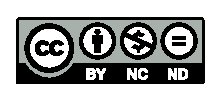
\includegraphics[width=1in]{Graphics/Cc-by-nc-nd_icon}} & {\small Este obra está bajo una licencia de \textbf{Creative Commons Reconocimiento-NoComercial-SinObraDerivada 4.0 Internacional}.	\url{https://creativecommons.org/licenses/by-nc-nd/4.0/}}\\
\end{tabularx}

\bigskip

\noindent
\textsf{\spacedlowsmallcaps{Contact}}

\noindent
{\raisebox{-0.33ex}{\ding{43}}}\,\mail{fjesusmartinez@ugr.es}

\cleardoublepage%*******************************************************
% Dedication
%*******************************************************
\cleardoubleemptypage
\thispagestyle{empty}
%\phantomsection 
\refstepcounter{dummy}
\pdfbookmark[1]{Dedication}{Dedication}

\vspace*{3cm}

\begin{flushright}
    \textit{Hazlo o no lo hagas, pero no lo intentes.} \\ \medskip
    --- El imperio contraataca
\end{flushright}


\medskip

\begin{flushright}
    \textit{A la memoria de Obdulia Mart\'inez.} \\ \smallskip
%    1939\,--\,2016
\end{flushright}
\cleardoublepage%*******************************************************
% Declaration
%*******************************************************
\refstepcounter{dummy}
\begin{otherlanguage}{spanish}
\chapter*{Declaración}

\thispagestyle{empty}
\bigskip
El doctorando \myName y los directores de la tesis \myProf y \myOtherProf garantizamos, al firmar esta tesis doctoral, que el trabajo ha sido realizado por el doctorando bajo la dirección de los directores de la tesis y hasta donde nuestro conocimiento alcanza, en la realización del trabajo, se han respetado los derechos de otros autores a ser citados, cuando se han utilizado sus resultados o publicaciones.  

\bigskip
\bigskip
\noindent\textit{\myLocation, \myTime}

\bigskip
\bigskip


\noindent\begin{minipage}[t]{0.45\textwidth}
\centering Directores de la Tesis: 

\bigskip
\bigskip
\bigskip
\bigskip

\myProf

\bigskip
\bigskip
\bigskip
\myOtherProf
\end{minipage} 
\hfill
\noindent\begin{minipage}[t]{0.45\textwidth}
\centering Doctorando: 

\bigskip
\bigskip
\bigskip
\bigskip

\myName
\end{minipage}

\end{otherlanguage}

%\cleardoublepage\include{FrontBackmatter/Foreword}
\cleardoublepage%*******************************************************
% Abstract
%*******************************************************
%\renewcommand{\abstractname}{Abstract}
\pdfbookmark[0]{Abstract}{Abstract}
\begingroup
%\let\clearpage\relax
%\let\cleardoublepage\relax
%\let\cleardoublepage\relax

\chapter*{Abstract}
The rise of neuroimaging in the last years has provided physicians and radiologist with the ability to study the brain with unprecedented ease. This led to a new biological perspective in the study of neurodegenerative diseases, allowing the characterization of different anatomical and functional patterns associated with them. \acf{CAD} systems use statistical techniques for preparing, processing and extracting information from neuroimaging data pursuing a major goal: optimize the process of analysis and diagnosis of neurodegenerative diseases and mental conditions.

With this thesis we focus on three different stages of the \ac{CAD} pipeline: preprocessing, feature extraction and validation. For preprocessing, we have developed a method that target a relatively recent concern: the confounding effect of false positives due to differences in the acquisition at multiple sites. Our method can effectively merge datasets while reducing the acquisition site effects. Regarding feature extraction, we have studied decomposition algorithms (independent component analysis, factor analysis), texture features and a complete framework called Spherical Brain Mapping, that reduces the 3-dimensional brain images to two-dimensional statistical maps. This allowed us to improve the performance of automatic systems for detecting Alzheimer's and Parkinson's diseases. Finally, we developed a brain simulation technique that can be used to validate new functional datasets as well as for educational purposes. 
%Guide: 
%\begin{center}
%	\url{https://plg.uwaterloo.ca/~migod/research/beckOOPSLA.html}
%\end{center}

\endgroup			

\vfill
%\cleardoublepage%*******************************************************
% Publications
%*******************************************************
\pdfbookmark[1]{Publicaciones}{publicaciones}
\chapter*{Publicaciones}%\graffito{This is just an early --~and currently ugly~-- test!}
Some ideas and figures have appeared previously in the following publications, that we divide here in articles and conference presentations. 

%\noindent Put your publications from the thesis here. The packages \texttt{multibib} or \texttt{bibtopic} etc. can be used to handle multiple different bibliographies in your document.

\begin{refsection}[ownpubs]
    \small
    \nocite{*} % is local to to the enclosing refsection
    \newrefcontext[sorting=ydnt]
    \printbibliography[heading=subbibliography, title={Articles}, type=article]
    \printbibliography[heading=subbibliography, title={Conferences}, type=inproceedings]
\end{refsection}

\cleardoublepage\include{FrontBackmatter/Acknowledgments}
\pagestyle{scrheadings}
\cleardoublepage%*******************************************************
% Table of Contents
%*******************************************************
%\phantomsection
\refstepcounter{dummy}
\pdfbookmark[0]{\contentsname}{tableofcontents}
\setcounter{tocdepth}{2} % <-- 2 includes up to subsections in the ToC
\setcounter{secnumdepth}{3} % <-- 3 numbers up to subsubsections
\manualmark
\markboth{\spacedlowsmallcaps{\contentsname}}{\spacedlowsmallcaps{\contentsname}}
\tableofcontents 
\automark[section]{chapter}
\renewcommand{\chaptermark}[1]{\markboth{\spacedlowsmallcaps{#1}}{\spacedlowsmallcaps{#1}}}
\renewcommand{\sectionmark}[1]{\markright{\thesection\enspace\spacedlowsmallcaps{#1}}}
%*******************************************************
% List of Figures and of the Tables
%*******************************************************
\clearpage

\begingroup 
    \let\clearpage\relax
    \let\cleardoublepage\relax
    \let\cleardoublepage\relax
    %*******************************************************
    % List of Figures
    %*******************************************************    
    %\phantomsection 
    \refstepcounter{dummy}
    %\addcontentsline{toc}{chapter}{\listfigurename}
    \pdfbookmark[0]{\listfigurename}{lof}
    \listoffigures

    \vspace{8ex}

    %*******************************************************
    % List of Tables
    %*******************************************************
    %\phantomsection 
    \refstepcounter{dummy}
    %\addcontentsline{toc}{chapter}{\listtablename}
    \pdfbookmark[0]{\listtablename}{lot}
    \listoftables
        
    \vspace{8ex}
%   \newpage
    
    %*******************************************************
    % List of Listings
    %*******************************************************      
      %\phantomsection 
%    \refstepcounter{dummy}
%    %\addcontentsline{toc}{chapter}{\lstlistlistingname}
%    \pdfbookmark[1]{\lstlistlistingname}{lol}
%    \lstlistoflistings 
%
%    \vspace{8ex}
       
    %*******************************************************
    % Acronyms
    %*******************************************************
    %\phantomsection 
    \refstepcounter{dummy}
    \pdfbookmark[0]{Acronyms}{acronyms}
    \markboth{\spacedlowsmallcaps{Acronyms}}{\spacedlowsmallcaps{Acronyms}}
    \chapter*{Acronyms}
    \begin{acronym}[MRC-AIMS]
	    \acro{PCA}{Principal Component Analysis}
	    \acro{ICA}{Independent Component Analysis}
	    \acro{FA}{Factor Analysis}
	    \acro{SPECT}{Single Photon Emission Computed Tomography}
	    \acro{CT}{Computed Tomography}
	    \acro{PET}{Positron Emission Tomography}
	    \acro{AD}{Alzheimer's Disease}
	    \acro{PD}{Parkinson's Disease}
	    \acro{PKS}{Parkinsonism}
	    \acro{ASD}{Autism Spectrum Disorder}
	    \acro{MRI}{Magnetic Resonance Imaging}
	    \acro{fMRI}{functional \acs{MRI}}
	    \acro{PLS}{Partial Least Squares}
	    \acro{SWPCA}{Significance Weighted Principal Component Analysis}
	    \acro{SBM}{Spherical Brain Mapping}
	    \acro{VBM}{Voxel Based Morphometry}
	    \acro{SPM}{Statistical Parametric Mapping}
	    \acro{SPM8}{Statistical Parametric Mapping Software, version 8}
	    \acro{CTL}{Control Subject}
	    \acro{VAF}{Voxels As Features}
	    \acro{CAD}{Computer Aided Diagnosis}
	    \acro{ADNI}{Alzheimer's Disease Neuroimaging Initiative}
	    \acro{PPMI}{Parkinson's Progression Markers Initiative}
	    \acro{VDLN}{Virgen de las Nieves Hospital}
	    \acro{VDLV}{Virgen de la Victoria Hospital}
	    \acro{MRC-AIMS}{Medical Research Council Autism Imaging Multicentre Study}
	    \acro{MNI}{Montreal Neurological Institute}
	    \acro{synT1}{simulated T1 - weighted Inversion Recovery}
	    \acro{qT1}{quantitative T1 - weighted}
	    \acro{qT2}{quantitative T2 - weighted}
	    \acro{GM}{grey matter}
	    \acro{GLM}{General Linear Model}
	    \acro{WM}{white matter}
	    \acro{CSF}{cerebro-spinal fluid}
	    \acro{ANOVA}{Analysis Of Variance}
	    \acro{SVD}{Singular Value Decomposition}
	    \acro{SVA}{Surrogate Variable Analysis}
	    \acro{SVM}{Support Vector Machine}
	    \acro{SVC}{Support Vector Classifier}
	    \acro{CBM}{Component Based Morphometry}
	    \acro{KDE}{Kernel Density Estimation}
	    \acro{MCI}{Mild Cognitive Impairment}
	    \acro{EM}{Expectation-Maximization}
	    \acro{PDF}{Probability Density Function}
	    \acro{CDF}{Cumulative Density Function}
	    \acro{FWE}{Family Wise Error rate}
	    \acro{RF}{radiofrequency}
	    \acro{SNR}{Signal-To-Noise Ratio}
	    \acro{rCBF}{regional Cerebral Blood Flow}
	    \acro{DAT}{Do\-pa\-mi\-ne Trans\-por\-ters}
	    \acro{FBP}{Filtered Back Projection}
	    \acro{FDR}{False Discovery Rate}
	    \acro{ROI}{Region of Interest}
	    \acrodefplural{ROI}{Regions of Interest}
	    \acro{ROC}{Receiver Operating Characteristics}
	    \acro{HMM}{Hidden Markov Model}
	    \acrodefplural{HMM}{Hidden Markov Models}
	    \acro{AC}{Anterior Commissure}
	    \acro{LBP}{Local Binary Patterns}
	    \acro{VRLBP}{Volumetric Radial \acs{LBP}}
	    \acro{AAL}{Automated Anatomical Labeling}
	    \acro{DTI}{Diffusion Tensor Imaging}
	    \acro{CV}{Cross-validation}
	    \acro{LOO}{Leave-One-Out}
	    \acro{TP}{True Positive}
	    \acro{FP}{False Positive}
	    \acro{TN}{True Negative}
	    \acro{FN}{False Negative}
	    \acro{KL}{Kullback-Leibler}
	    \acro{MWW}{Mann-Whitney-Wilcoxon}
	    \acro{EVD}{eigen-value decomposition}
	    \acro{SWEDD}{subjects without evidence of dopaminergic deficit}
	    \acro{GLCM}{Grey Level Co-occurrence Matrix}
	    \acro{RBF}{Radial Basis Function}
	    \acro{MVN}{Multivariate Normal distribution}
    \end{acronym}                     
\endgroup

%********************************************************************
% Mainmatter
%*******************************************************
\cleardoublepage\pagenumbering{arabic}
%\setcounter{page}{90}
% use \cleardoublepage here to avoid problems with pdfbookmark
\cleardoublepage
\ctparttext{In this part, we will focus on the motivation of this Thesis, examining the state-of-the-art methodology used in clinical practice. We will also provide a brief medical background on the diseases studied in this work, as well as an examination of the computational methodology in neuroimaging. }
\part{Introduction}
%************************************************
\chapter{Introduction}\label{ch:introduction}
%************************************************
\section{Motivation}
In recent years, there has been a rise in the use of neuroimaging in the clinical practice. It has improved and speeded the procedure of diagnostic, providing unprecedented insight into the brain. Neuroimaging is very extended in research as well. Different fields such as psychiatry, neurology, psychology, behavioural science or biology make extensive use of brain imaging in their studies. 

The basis of these studies are common: a selection procedure by which a representative set of subjects is recruited, the fulfilment of an experiment on (or by) each subject and a statistical analysis of the acquired data. Particularly, when studying a certain disease, it is common to recruit subjects affected by the disease and non-affected, healthy subjects, usually known as \acp{CTL}. Then, in this typical example, both affected and \acp{CTL} are scanned, and brain anatomy or function is analysed using statistical tools. The result of this analysis is a list of significant differences between structure or function that could be linked to the disease. 

\ac{CAD} systems provide a set of tools to help setting up and performing these studies. It is currently a thriving area of research involving multidisciplinary teams, combining computer science, mathematics, medicine, artificial intelligence, statistics, machine learning, and many others \cite{Martinez-Murcia2016}. The main aim is to assist clinicians in the procedure of diagnosis and study of the diseases by providing software that can effectively recognize disease patterns, characterize differences and make predictions. 

One fundamental issue often found in this studies is the sample size. The number of subjects frequently ranges from tens to hundreds, whereas the number of features (namely voxels) to be analysed can add up to millions. This causes the so-called \emph{Small Sample Size Problem} \cite{Duin2000} which negatively affects the statistical power of any experiment performed using these datasets \cite{Button2013}. 

\begin{figure}
\centering
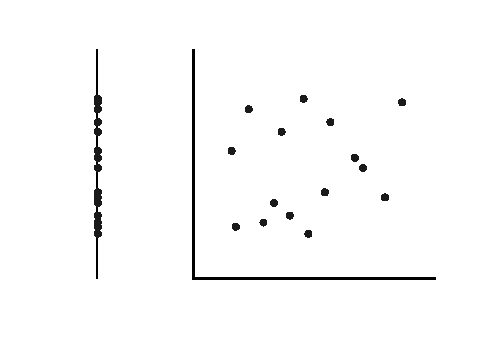
\includegraphics[width=0.6\linewidth]{Graphics/ch1/smallsample}
\caption[Illustration of one and two-dimensional spaces.]{Illustration of the separation between points in one-dimensional and two-dimensional spaces.}
\label{fig:smallsample}
\end{figure}


\section{The Small Sample Size Problem}\label{sec:smallsamplesize}
The \textit{Small Sample Size Problem} refers to a problem that arises when the proportion between number of subjects and number of features is large. Think of, \eg, 15 points in a one-dimensional line, as in Figure~\ref{fig:smallsample}. If we think of a subject as a vector, we would have 15 subjects in a one-dimensional space. Now, imagine that we add a second dimension. It is easy to see that our subjects would be farther than in the two-dimensional world. And the same would happen if we move to four, ten or thousands of dimensions. The farther our points are, the more difficult is for a statistical tool to extract information. That is what we call \textit{almost empty spaces} \cite{Stoeckel04}, in contrast to \textit{dense spaces}, where points are closer. 

Neuroimaging provides hundreds of thousands, or even millions of voxels, in what could mean millions of features. That implies that any calculation performed in those almost empty spaces will eventually lack information. This implies a loss of statistical power of the methods used, usually producing false negatives (the system is unable to detect real signal) and false positives (the system detects signal where there is not). These are known in statistics as Type I and Type II errors respectively. 

In differential diagnosis studies, the small sample size problem leads to wrong conclusions about where real differences are located. This, in addition to untracked confounding variables are one of the fundamental sources of non-re\-pro\-du\-ci\-bi\-li\-ty un current neuroimaging studies \cite{Button2013}. 

The solution might seem straightforward: increase sample size. But this is not always possible, since neuroimaging studies do their best at recruiting as many people as they can with a limited budget. Many efforts have been put into establishing multi-centre collaborations that allow the recruitment of a larger population, but despite offering a higher statistical power, these studies still suffer from a number of confounding variables such as population bias or scanner differences \cite{haar2014anatomical}. In Chapters~\ref{ch:swpca} and \ref{ch:simulation} we explore different approaches to this solution. 

Another option involves reducing the number of features, via feature selection or feature extraction. This has been widely used in computed-aided methodology for neuroimaging \cite{DeMartino2007,xu2009source,Gorriz2010,Illan2011,Martinez-Murcia2016} with great success, and solutions using this approach will be treated in Chapters~\ref{ch:decomposition}, \ref{ch:texture} and \ref{ch:sbm}. 

The Small Sample Size problem is directly related to the \textit{Curse of Dimensionality} \cite{Krishnaiah1982}, which proves that, in contrast to what could be expected, once a certain classifier performance has been achieved, it holds or even decreases when feeding more features to the classifier. The problem also affects statistical hypothesis testing, a tool widely used for inference in neuroimaging, in what is known as the \textit{Multiple Comparisons} problem \cite{Benjamini2010}, a particular field that is still being studied. 

% DONE
\section{Aims and Objectives}\label{sec:overview}
This thesis aims to contribute new approaches to overcome the small sample size problem in neuroimaging. This can provide more accurate \ac{CAD} systems by reducing the number of false positives, increasing the reliability of their results. 

We will take two different approaches, as commented in previous sections: increasing the sample size and reducing the feature space. Therefore, we can define the following objectives: 

\begin{itemize}
	\item Develop and evaluate algorithms that reduce the feature space, in which is usually known in the field as feature extraction and feature selection strategies. 
	\item Develop and evaluate new strategies to increase the sample size in neuroimaging studies. 
\end{itemize}

Many strategies have been proposed . 

In this thesis we plan to tackle the Small Sample Size problem in two different approaches. 


First strategy: decrease the number of features -> Feature extraction. This is the subject of Decomposition techniques, Texture Analysis and \ac{SBM}. 

Second strategy: increase the sample size. Most popular option: multi-site studies where subjects are acquired using similar techniques at different sites. This poses a major problem: inhomogeneities, etc. To overcome this we propose the \ac{SWPCA}. Other option: simulate new subjects from the existent database, in order to increase sample size.



The aim of the work, i.e. the overall purpose of the study, should be clearly and concisely defined.

Aims:
Are broad statements of desired outcomes, or the general intentions of the research, which 'paint a picture' of your research project
Emphasize what is to be accomplished (not how it is to be accomplished)
Address the long-term project outcomes, i.e. they should reflect the aspirations and expectations of the research topic.
Once aims have been established, the next task is to formulate the objectives. Generally, a project should have no more than two or three aims statements, while it may include a number of objectives consistent with them.

Objectives are subsidiary to aims and:

Are the steps you are going to take to answer your research questions or a specific list of tasks needed to accomplish the goals of the project
Emphasize how aims are to be accomplished
Must be highly focused and feasible
Address the more immediate project outcomes
Make accurate use of concepts
Must be sensible and precisely described
Should read as an 'individual' statement to convey your intentions
Here is an example of a project aim and subsidiary objectives:


Obj: provide more accurate CAD systems by reducing the number of false positives, increasing the reliability of their results. 

1 - Develop and evaluate different strategies for reducing the feature space. 
2 - Develop and evaluate different strategies for safely increasing the sample size. 

The overall goal of this thesis was to contribute to the emerging field of statistical eco-
toxicology, environmental risk assessment and environmental monitoring. The main
objectives were (i) to scrutinise new methods in statistical ecotoxicology and effect as-
sessment, (ii) explore risk dynamics using available monitoring data and (iii) provide
tools to deal with and integrate big data in ERA. Figure 1.1 provides a conceptual
overview on ERA and environmental monitoring as outlined in the previous sections,
as well as the parts considered in this thesis and their relationships.

\section{Contributions}
Some ideas and figures have appeared previously in the following publications, that we divide here in articles and conference presentations. 

%\noindent Put your publications from the thesis here. The packages \texttt{multibib} or \texttt{bibtopic} etc. can be used to handle multiple different bibliographies in your document.

\begin{refsection}[ownpubs]
	\small
	\nocite{*} % is local to to the enclosing refsection
	\newrefcontext[sorting=ydnt]
	\subsection{Articles}
	\printbibliography[env=nolabelbib,heading=none,keyword=own, title={Articles}, type=article]
	\subsection{Conferences}
	\printbibliography[env=nolabelbib,heading=none,keyword=own, title={Conferences}, type=inproceedings]
	\subsection{Books}
	\printbibliography[env=nolabelbib,heading=none,keyword=own, title={Books}, type=inbook]
\end{refsection}

\section{Organization of this Thesis}

\begin{figure}
\centering
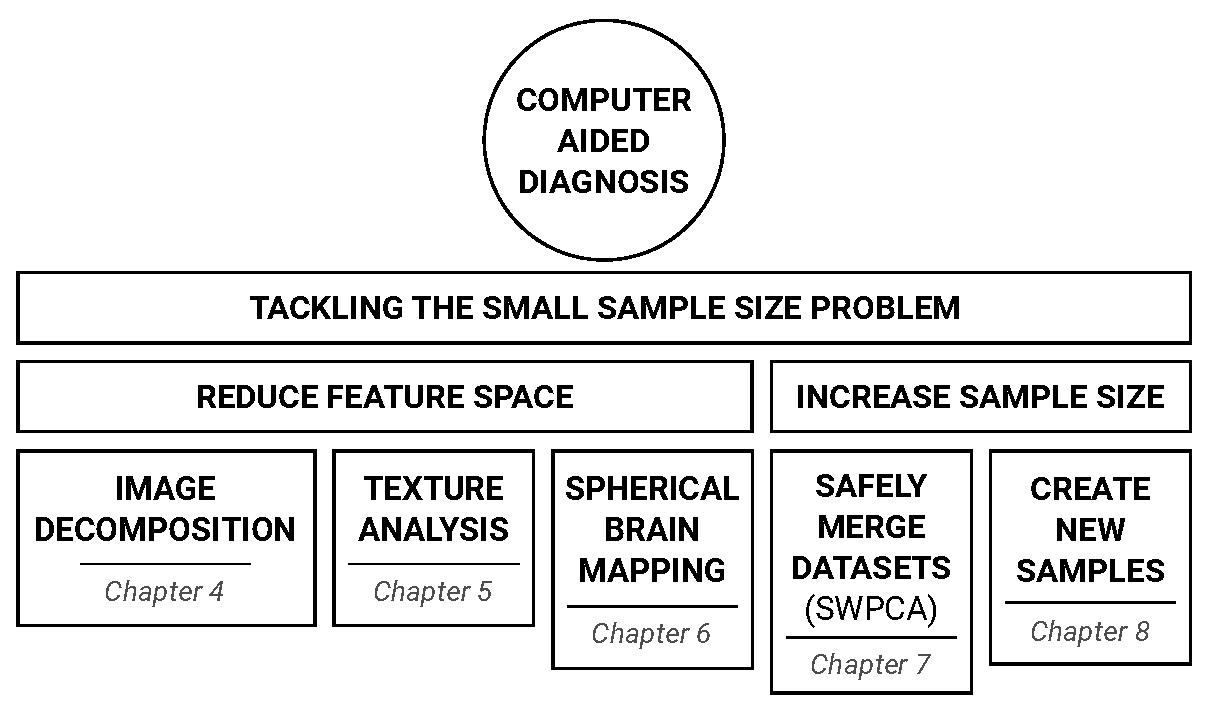
\includegraphics[width=0.7\linewidth]{Graphics/ch1/outline}
\caption[Structure of the thesis.]{Structure and connexions between the different strategies proposed in this thesis, organized by chapters and parts.}
\label{fig:outline}
\end{figure}

This thesis work is organized in four parts plus appendices, each of which is subdivided in several chapters. In the first part, we introduce the motivations and main aims of this work (Chapter~\ref{ch:introduction}), examine the state of the art in medicine, neuroimaging and \ac{CAD} systems (Chapter~\ref{ch:stateofart}) and present a general methodology that will be followed throughout this thesis, including preprocessing and evaluation (Chapter~\ref{ch:preprocessing}). 

Parts \ref{part:feature} and \ref{part:increase} refers to each of the solutions outlined above, and disaggregated in Figure~\ref{fig:outline}. In part~\ref{part:feature} we focus on the feature reduction techniques, including decomposition methods (Chapter~\ref{ch:decomposition}), texture analysis (Chapter~\ref{ch:texture}), and the novel algorithm Spherical Brain Mapping (Chapter~\ref{ch:sbm}). On the other hand, Part~\ref{part:increase} is focused on two different strategies used to increase the sample size: the Significance Weighted Principal Component Analysis algorithm (Chapter~\ref{ch:swpca}), used to safely merge structural images acquired at different centres, and a neuroimage simulation algorithm (Chapter~\ref{ch:simulation}) that can be used to extend existing functional datasets. 

Finally, in Part~\ref{part:dicussion} we provide a general discussion of the results presented in this thesis, conclusions about the methods and prospective work that could be performed with this basis. 

% !TEX TS-program = pdflatex
% !TEX root = ../ArsClassica.tex
%*****************************************
\chapter{State of the Art}\label{ch:stateofart}
%*****************************************
We have already stated the motivation and objectives of this thesis. Now, we will describe in detail some of the more relevant issues for the state of the art. First, in Section~\ref{sec:neuroimaging}, we will make an introduction to the different neuroimaging modalities used in our experiments. Afterwards, we will provide some insights into the neurological and psychiatric disorders treated here in Section~\ref{sec:disorders} or the most extended voxel-wise analyses used in the neuroimaging community at Section~\ref{sec:vwanalyses}. Finally, at Section~\ref{sec:machinelearning} we will explore recent contributions to the field that use Machine Learning. 

\section{Introduction to Neuroimaging}\label{sec:neuroimaging}
Medical imaging refers to all types of 2D, 3D and 4D images used in clinical practice. These involve many different modalities, among them X-rays, ultrasound, endoscopy, microscopy, etc. In neuroimaging, the most extended is by far \ac{MRI}, which provides intensity maps that represent the internal structure of the brain. Other modalities are aimed at studying the function of the brain, by injecting radioactive ligands that, linked to a receptor, can measure its distribution. This is the case of \ac{PET} and \ac{SPECT}.

\subsection{Magnetic Resonance Imaging}
\acf{MRI} is perhaps the most widespread in neuroimaging, given its ability to visualize both structural and functional (in functional \ac{MRI}) properties of the brain, and, in contrast to other imaging modalities, is considered non-invasive. \ac{MRI} uses strong magnetic fields to excite certain atomic nuclei, that can absorb and emit this energy. 

\begin{figure}[htp]
	\centering
	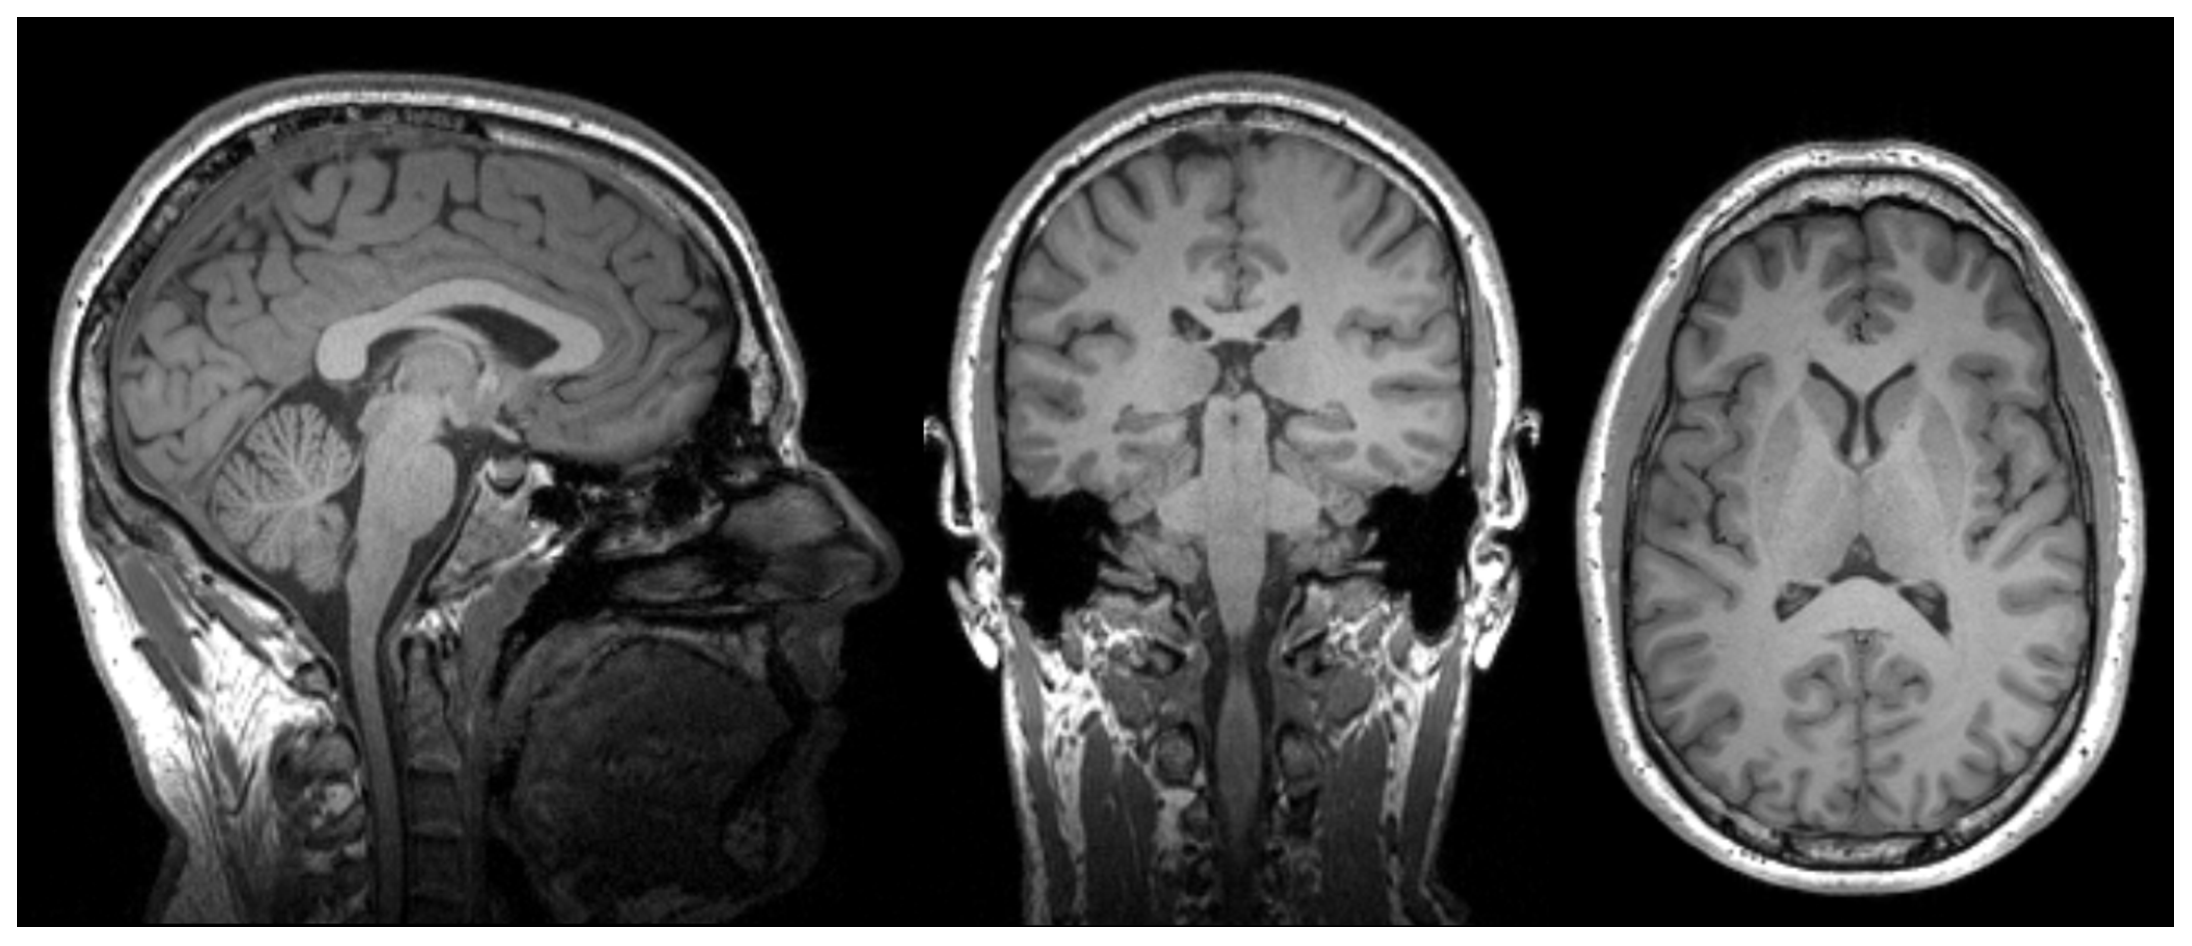
\includegraphics[width=0.7\linewidth]{Graphics/ch2/example_MRIT1}\\
	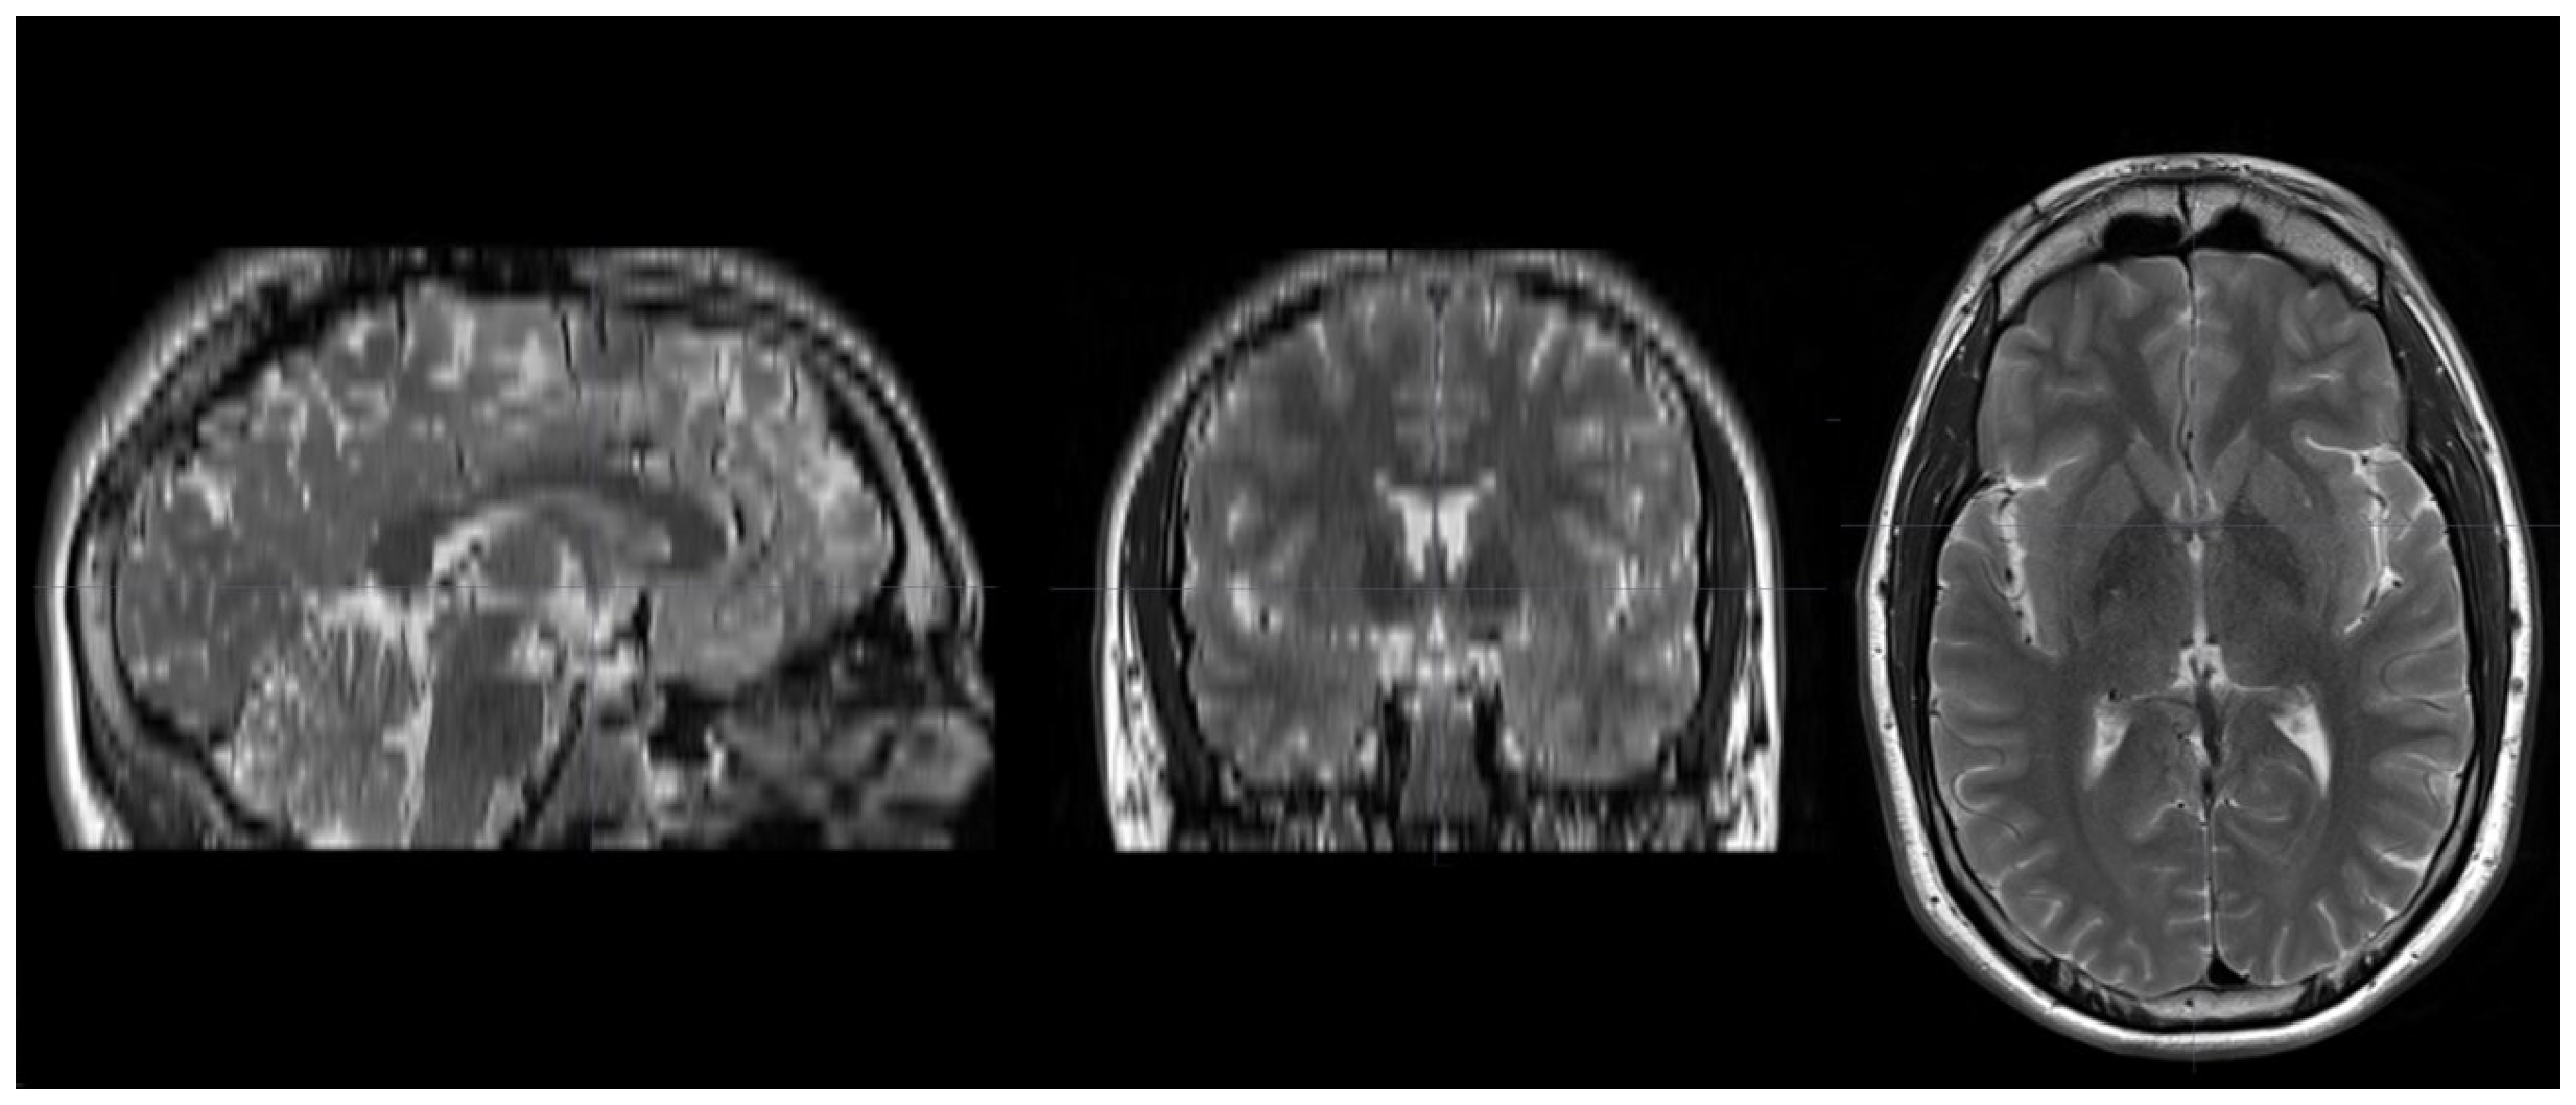
\includegraphics[width=0.7\linewidth]{Graphics/ch2/example_MRIT2}
	\caption[Example of T1 and T2-weighted MRI images.]{Example of T1 and T2-weighted MRI images of the same subject (me).}
	\label{fig:example_MRI}
\end{figure}

\ac{MRI} combines the magnetic field with a \ac{RF} emission to excite the atomic nuclei present in corporal structure, resulting in a image of the distribution of certain atoms in the body. Most \ac{MRI} use hydrogen atoms, since they are present in water (which adds up to around 70\% of body mass) and the signal derived is stronger than other atoms, increasing the \ac{SNR}, and therefore, the image quality. 

The procedure uses a strong magnetic field $B_0$ to align the magnetic moment of the hydrogen nuclei in parallel or anti-parallel (depending of their initial spin). This way, the magnetic moment of all nuclei will increase up to a stable state, in contrast to their null value in absence of $B_0$. Within this magnetic field, the hydrogen atoms precess around an axis along the direction of the field. 

A given nuclei has a resonance frequency which is proportional to the intensity of $B_0$, which, by using strong fields, allow us to resonate hydrogen far below potentially damaging frequencies. The precession frequency is determined by the Larmor equation (\ref{eq:lamor}):

\begin{equation}\label{eq:lamor}
f_0 = \frac{\gamma}{2\pi } B_0 
\end{equation}
where $\gamma$ depends on the nuclei, which in the case of hydrogen, $\gamma = 42.6$ MHz/T. When a subject is introduced in the \ac{MRI} scanner, it is submitted to the magnetic field $B_0$, so that the hydrogen nuclei are aligned to the field, with a precession frequency $f_0$. Then, a \ac{RF} pulse of the same frequency is generated, which is then absorbed by the nuclei, forcing them to place perpendicular to the field. Once the \ac{RF} emission is interrupted, the nuclei return to its equilibrium state by means of a procedure called relaxation. In this procedure, they emit part of the absorbed energy, which is then captured by a \ac{RF} receptor. Usually, position information is encoded in the \ac{RF} signal by varying $B_0$ using gradient coils. 

The \ac{RF} signal is measured during the relaxation time, and two different relaxation times are set: the T1 (spin-lattice) relaxation time and the T2 (spin-spin) relaxation time. The T1 time is the time during which nuclei emit energy to the adjacent tissue and realign to the longitudinal plane (z axis), whereas the T2 time refers to the time when nuclei realign to the transversal plane (y axis). These times are used to create T1-weighted and T2-weighted images (see Figure~\ref{fig:example_MRI}). T1-weighted images allow to distinguish between \ac{GM} and \ac{WM} in the cerebral cortex, to identify fatty tissue, and generally, obtain structural information. Conversely, T2-weighed images are used to assess \ac{CSF} or to visualize and identify \ac{WM} lessions. 

\subsection{Single Photon Emission Computed Tomography}
The \acf{SPECT} is based on the principles of \ac{CT}, by which a series of signal acquisition at different angles can be reconstructed back into a bidimensional distribution of the signal. In \ac{SPECT}, a gamma photon emitting radioisotope is linked to a pharmaceutical that binds to a given biomarker, generating a radiopharmaecutical or agent. This agent is injected into the patient, and after a certain time in which the radiopharmaceutical is distributed, the patient is introduced into the \ac{SPECT}-\ac{CT} scan. 

Afterwards, the scanner performs a series of acquisitions at different planes and angles from the body, from which the gamma signal is measured. For each plane, all acquisitions at each angle are pooled and a single two-dimensional image is reconstructed using a \ac{FBP} algorithm, or Radon inversion formula \cite{Herman2009l}, which derives from the Fourier's Theorem. A total of 180 projections per plane, using an angular resolution of 2 degrees, are usually taken. 

There exist a number of radiopharmaceutical used in clinical practice, and therefore, we will focus on the two varieties used in this thesis. First, we use an agent called $^{99m}$Tc-HMPAO, which consists of two stereoisomers of hexametazime (HMPAO) linked to the radioisotope technetium 99-metastable. This agent is usually used to assess \ac{rCBF}, which can be used to diagnose neurological diseases or cancer. 

\begin{figure}[htp]
	\centering
	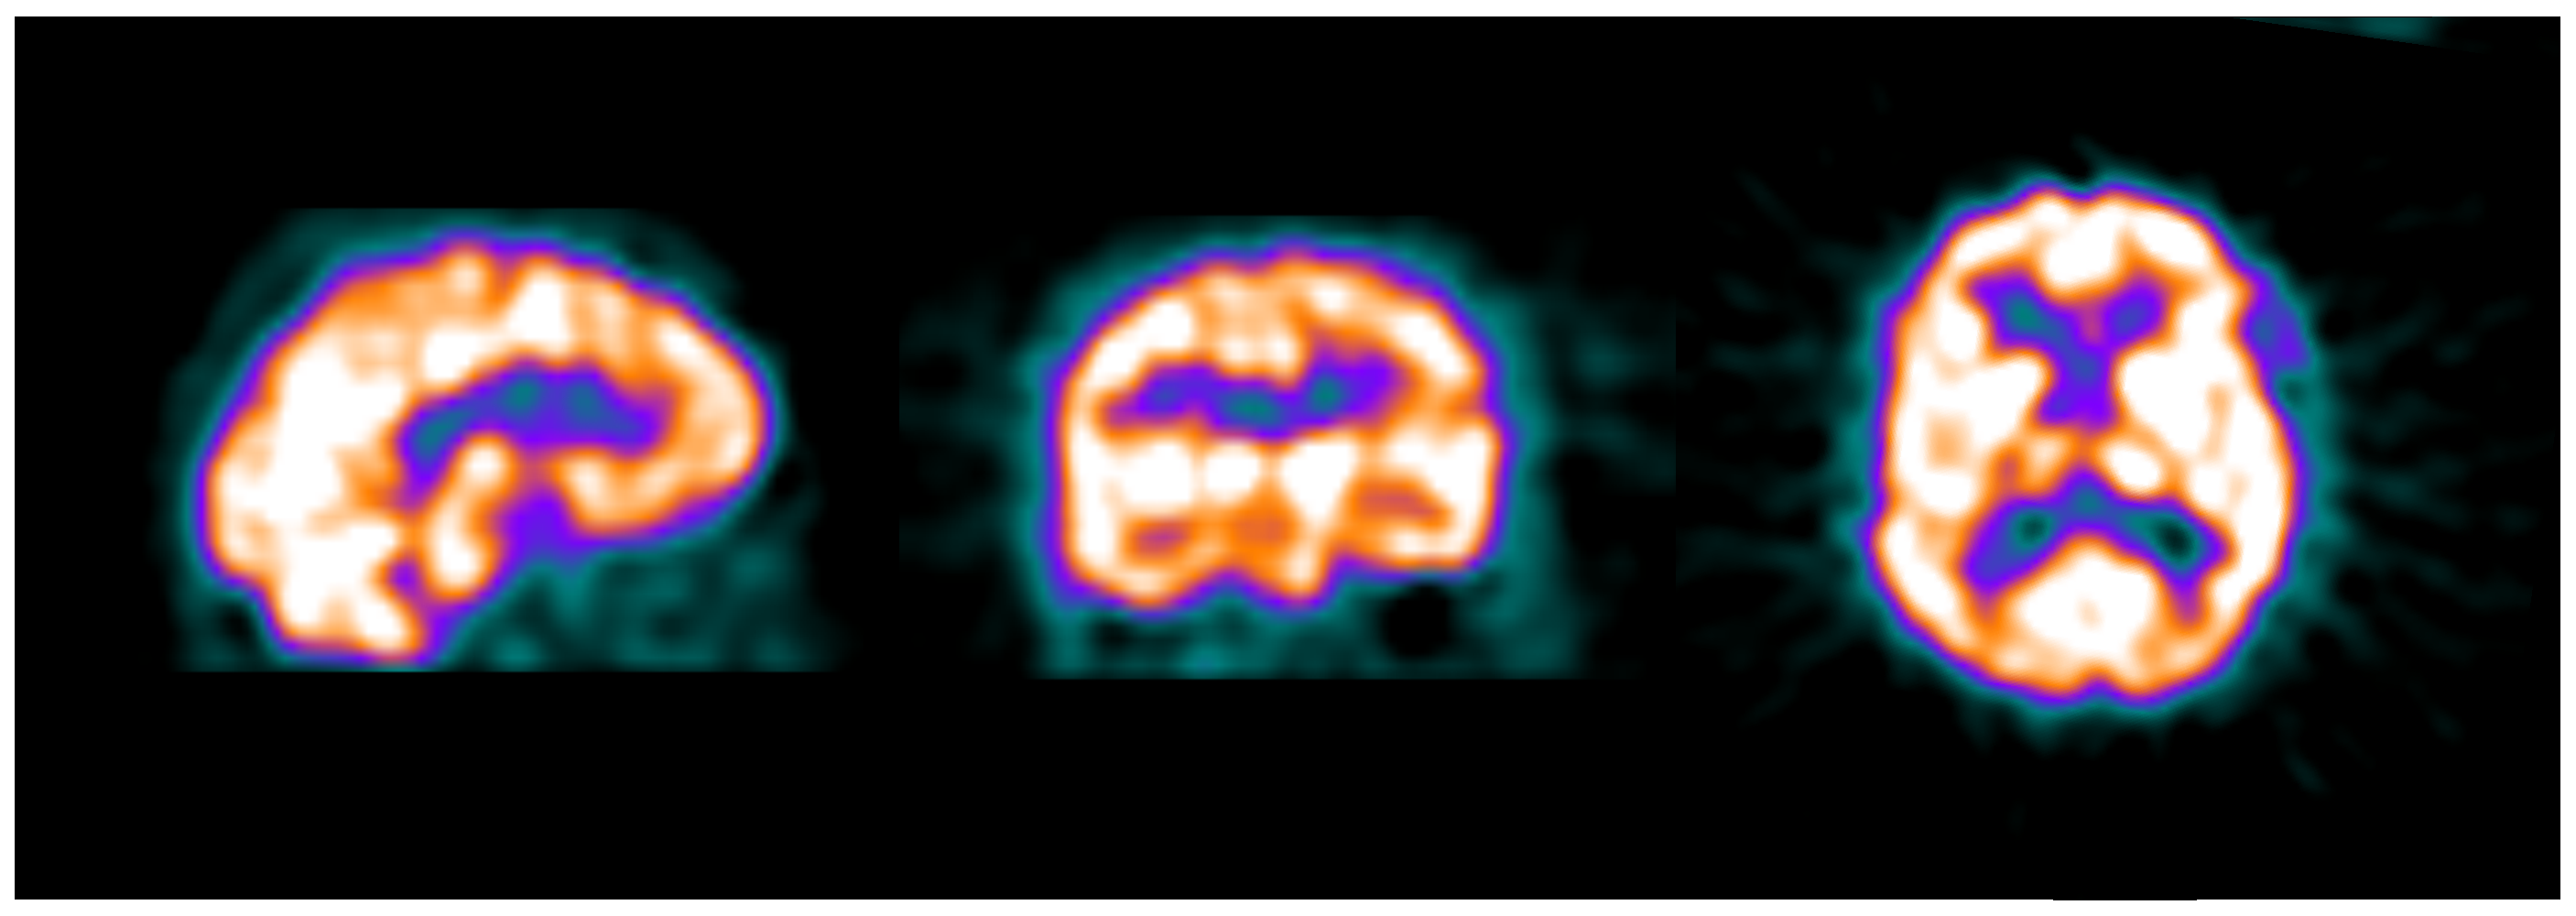
\includegraphics[width=0.7\linewidth]{Graphics/ch2/example_SPECT}\\
	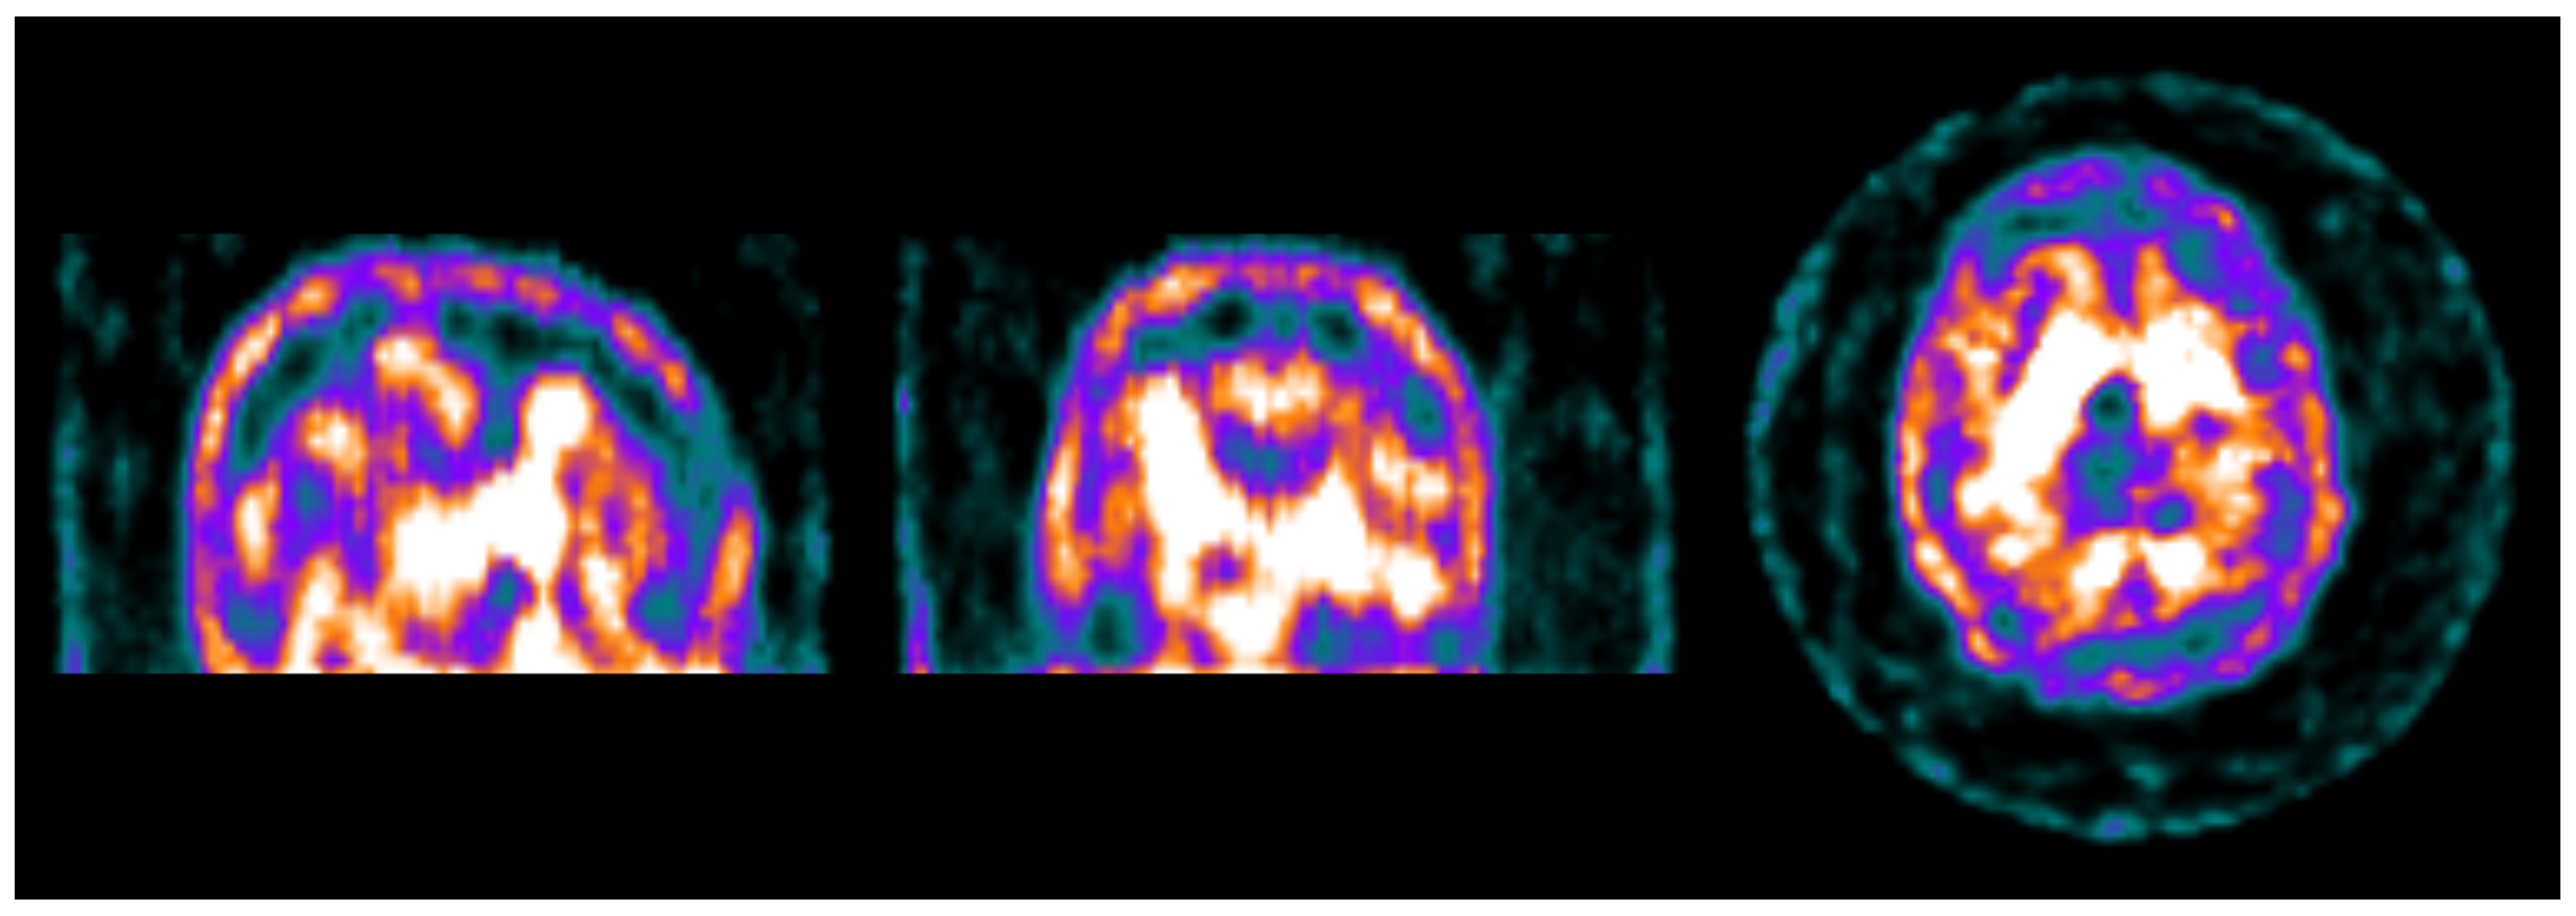
\includegraphics[width=0.7\linewidth]{Graphics/ch2/example_DaTSCAN}
	\caption[Example of SPECT images.]{Example of SPECT images, a SPECT-HMPAO and a SPECT-DaTSCAN.}
	\label{fig:example_SPECT}
\end{figure}

Additionally, we use images generated using the agent Ioflupane ($^{123}$I), a cocaine analog with high binding affinity for \ac{DAT}. It is used fundamentally in the assessment of \ac{PD}, given that the disease is associated with a loss of dopaminergic neurons in the striatal region. 

\subsection{Positron Emission Tomography}
The \acf{PET} is a technique similar to \ac{SPECT}, but in this case, the agent used and the equipment is designed to deal with a pair of gamma photons resulting of the annihilation of a positron with its corresponding antiparticle, the electron. The pair of photons are generated in opposite directions, and the detection depends on them being simultaneously or coincidently detected at the receptor. The receptor comprises a scintillator which emits light when the gamma photon incides, and a detector, usually a photomultiplier tube or silicon avalanche photodiodes.

It uses the same \ac{FBP} algorithm as \ac{SPECT} in the reconstruction of the images, and a similar strategy for acquiring the signal at different angles. However, the amount of data is smaller than in \ac{SPECT}, and therefore, the reconstruction procedure is harder. As a result, \ac{PET} scanner operation is considered more costly than \ac{SPECT} \cite{Carlson2016}.  

\begin{figure}[htp]
	\centering
	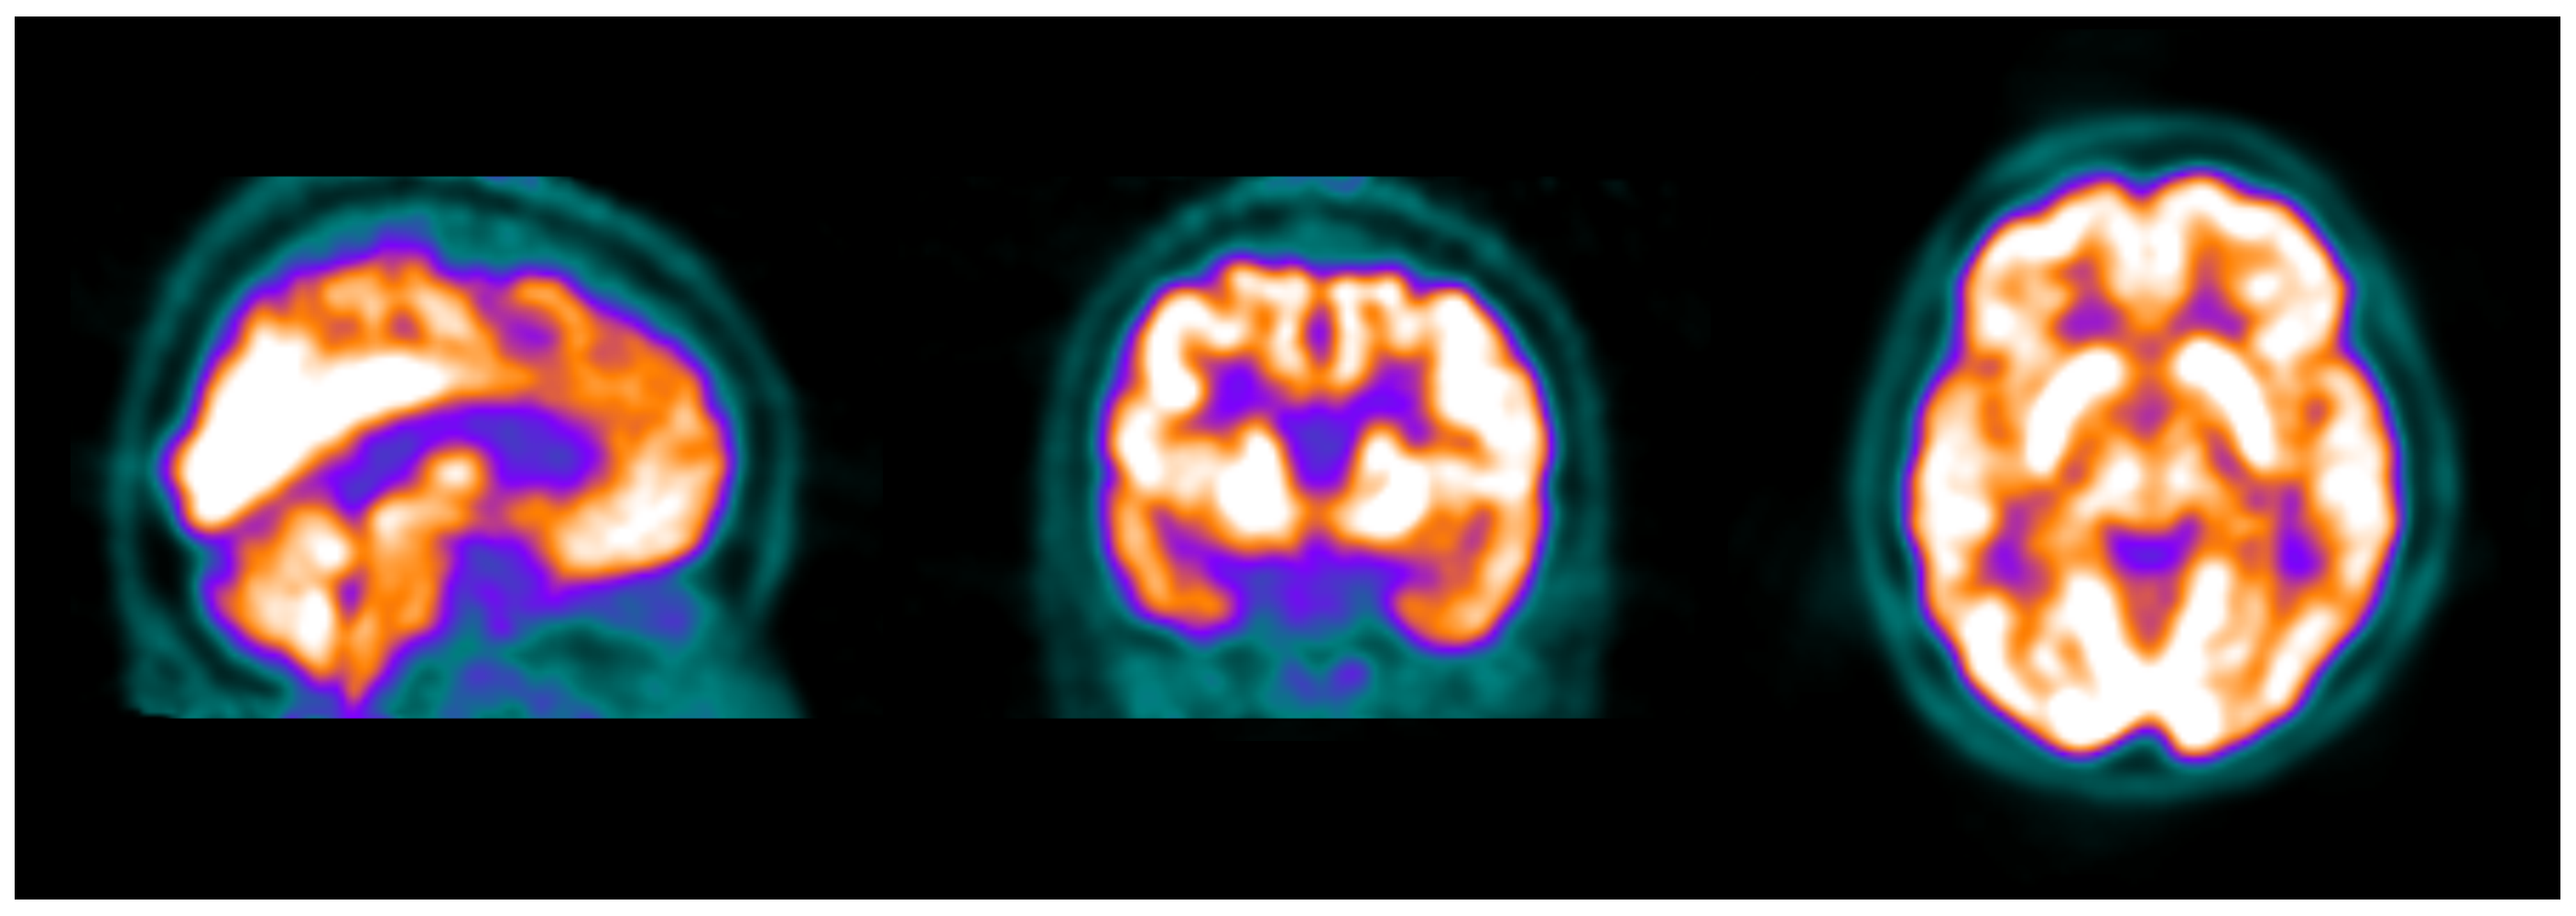
\includegraphics[width=0.7\linewidth]{Graphics/ch2/example_PET}
	\caption[Example of a PET-FDG image.]{Example of a PET-FDG image.}
	\label{fig:example_PET}
\end{figure}

The agent used in the images that we have processed is PET-FDG, also known as Fludeoxyglucose ($^{18}$F). It is a glucose analogue that allows us to measure the glucose metabolism in the brain. It is widely used in neurology \cite{Newberg2002} and cancer detection \cite{Kelloff2005}, since it can be correlated with cellular activity. 

\section{Medical Background}\label{sec:disorders}
\subsection{Alzheimer's Disease}
\acf{AD} is the most common cause of dementia in the world, with more than 46 million people affected, and it is likely to increase up to 135.5 million by 2050 \cite{Association2016}. Its causes are still not clear, but it is characterized by deposits of high amounts of structures such as Amyloid-$\beta$ (A$\beta$) plaques or neurofibrillary tangles accompanied by synaptic dysfunction and neurodegeneration that eventually lead to cell death \cite{Ballard2011,Sevigny2016}.

Diagnosis of \ac{AD} is often based on the clinical history of the patient, using cognitive tests along with medical imaging and blood tests. A definite diagnosis can only be addressed post-mortem, via a direct examination of the brain tissue \cite{Ballard2011}. Cognitive tests such as \textit{Mini Mental State Exam} or \textit{Clinical Dementia Ratio} are widely used in clinical practice. 

Initial symptoms of \ac{AD} are often mistaken for normal ageing, leading to a state known as \acf{MCI}. Not all \ac{MCI}-affected subjects develop \ac{AD}. In fact, the prediction of \ac{MCI} conversion is the most urging challenge in \ac{AD} research, since an early diagnosis can lead to an improvement in life expectancy and quality of life of the patients. 

% Rewrite
\ac{MRI} brain images have been extensively used in the diagnosis of \ac{AD} by assessing neurodegeneration on \ac{GM} and \ac{WM} tissues. Research has shown in \cite{Baron2001,Misra2009,Pievani2013,Dubois2007} that neurodegeneration in Alzheimer's Disease mainly occurs in the \ac{GM} tissue. Particularly grey matter loss has been described in the Hippocampus and Parahippocampal lobes, according to the NINCDS-ADRDA criteria for AD diagnosis \cite{Dubois2007}, with further atrophy described in the medial temporal structures, the Posterior Cingulate gyrus and adjacent Precuneus \cite{Baron2001}. Moreover, significantly lower volumes of certain regions in \ac{GM} and \ac{WM} have been considered a promising biomarker and predictor of the progression of \ac{AD} in a longitudinal study involving \ac{MCI} patients \cite{Misra2009}, and some structures in the striatum (putamen and caudate nucleus) have shown important volume abnormalities \cite{Pievani2013}. All these data suggest that many of the symptoms of \ac{AD} can be observed in anatomical \ac{MRI} images even in early stages of the disease, which could be of great help in its successful diagnosis and treatment. 

Nuclear imaging, such as \ac{PET} or \ac{SPECT}, have also been used in clinical practice, especially to discard other diseases. In typical \ac{PET}-FDG or \ac{SPECT}-HMPAO, \ac{AD} is characterized by reduced brain activity in bilateral regions, such as the posterior cingulate gyri and precunei, as well as the temporo-parietal region \cite{Claus1994}. It also affects the frontal cortex and the whole brain in severe cases \cite{Leon1983,Kogure2000}. 

Recently, new more specific radiopharmaceuticals have been developed, among them the Pittsburgh compound B (PiB). This drug binds to fibrillar A$\beta$ allowing \textit{in vivo} visualization of A$\beta$ plaques in the brain \cite{Ikonomovic2008}. However, due to their technical requirements -a relatively small half-life of the radioactive element-, they are unusual in clinical practice. 

% DONE

\subsection{Parkinsonism}
\acf{PKS} or Parkinsonian Syndrome is the second most common neurodegenerative disease in the world, with a prevalence of 1-3\% in the elder population (over 65 years)\cite{Eckert2007}. It is characterized by hypokinesia, rigidity, tremor and postural instability \cite{Eckert2007}. It is not a single disease itself, but a wide range of conditions that share similar symptoms. The most common cause of \ac{PKS} is \acf{PD}, but other possible causes include toxins, a few metabolic diseases, and other extrapyramidal syndromes such as Multiple System Atrophy, Progressive Supranuclear Palsy or Cortico-Basal Degeneration \cite{Christine2004,tatsch2008extrapyramidal}. 

\subsubsection{Parkinson's Disease}
The etiology of \acf{PD} involves the progressive loss of \acf{DAT} of the nigrostriatal pathway. This causes a decrease in the dopamine content of the striatum, since the pathway connects the substantia nigra to the striatum. 

In \ac{PD}, structural imaging such as \ac{MRI} has limited value, since structural abnormalities can be seen only in the latter stages. Nevertheless, in molecular imaging, a number of radiopharmaceuticals have been proposed to assess the levels of pre and post-synaptic \ac{DAT} at the striatum. Among them, the $^{123}$I-ioflupane (better known by its tradename DaTSCAN) is perhaps the most popular. DaTSCAN binds to the \ac{DAT} at the striatum \cite{Winogrodzka2003,PunalRioboo2007,Eckert2007}, allowing the estimation of \ac{DAT} density by means of a \ac{SPECT} scanner. In DaTSCAN images, a reduced uptake at the striatum is a clear indication of \ac{DAT} loss, and therefore, of \ac{PD} \cite{PunalRioboo2007}.
  
\subsubsection{Extrapyramidal Syndroms}
Among the extrapyramidal syndroms of \ac{PKS}, the most relevant diagnoses are Multiple System Atrophy, Progressive Supranuclear Palsy and Cortico-Basal Degeneration \cite{tatsch2008extrapyramidal}. An accurate diagnosis can positively impact in the health of these patients, avoiding wrong treatment decisions. 

Structural imaging, as in the previous case, has little value here. To establish a differential diagnosis with \ac{PD}, different drugs have been proposed. DaTSCAN is widely used to assess pre-synaptic dopaminergic loss, but in a post-synaptic level, one of the most extended is $^{18}$F-DMFP-PET \cite{Segovia2016a}. However, in this thesis we have focused only on the pre-synaptic level, and therefore, in the diagnosis of \ac{PD}. 

\subsection{Autism Spectrum Disorder}
\acf{ASD} is a neurodevelopmental syndrome characterized by social and communication impairment as well as restricted, repetitive patterns of behaviour, interests or activities. Its origins are still unknown, although research suggest \cite{Szatmari1999} that there exist genetic risk factors. 

The evidence of either functionally or structurally affected areas in the brain is a major concern \cite{Ecker2014,haar2014anatomical}. In the latter years, many strategies have been explored to recruit large samples in order to detect significant differences between affected and non-affected subjects. This has been addressed by initiatives such as the \ac{MRC-AIMS} \cite{Ecker2012,Ecker2013} or the Autism Brain Imaging Data Exchange (ABIDE) \cite{DiMartino2014}. 


\section{Voxelwise Analyses}\label{sec:vwanalyses}
Traditional analysis of neuroimaging involves visual analysis by experts clinicians, or semi-quantitative analysis of \acp{ROI}. With the rise of neuroimaging in the mid-nineties, some computer-aided solutions appeared, of which the most extended are the widely known \acf{SPM} \cite{Friston1994} and its extension to structural imaging \acf{VBM} \cite{Ashburner2000}. 

\subsection{Statistical Parametric Mapping}
\acf{SPM} is a new methodology to automatically examine differences in brain activity in functional imaging studies involving \ac{fMRI} or \ac{PET}, firstly proposed by Friston in \cite{Friston1994}. The technique can be applied either to static images (e.g., \ac{PET}) or timeseries (\ac{fMRI}), using inference techniques based on hypothesis testing, in order to construct the \ac{GLM} that better describes the variability in the data. 

Statistical hypothesis testing involves constructing a pair of hypotheses: $H_0$, or the null hypothesis, that states no relationship between variables; and $H_1$, the alternative hypothesis. In neuroimaging, $H_0$ usually means that there are no relevant differences between classes (for example, between patients affected by \acf{AD} and \ac{CTL}), and $H_1$ implies that there is a significant difference. Many different tests such as massive univariate $t$-Test or \ac{ANOVA} (see Chapter~\ref{ch:decomposition} for more information on these techniques) can be used in the \ac{SPM} software \cite{spm_book}, by using a design matrix that describes a $t$ or $F$ based contrast (for $t$-Test and \ac{ANOVA} respectively). These terms are generally referred to as $Z$-values, namely the signed number of standard deviations an observation is above the mean. 

The test are computed voxel-wise, from which a $p$-value can be obtained, nominally the probability of obtaining equally or more extreme $Z$ values that the one actually found.
$p$-values are very extended in neuroimaging, representing the probability of a $Z$ value being equal or more extreme than the reference value given. In many studies $p < 0.05$ is used for measuring statistical significance, which means that only a 5\% of the times a experiment is repeated we would obtain that result or a more extreme one. The use of the significance threshold $\alpha=0.05$ implies that any voxel with a $p$-value smaller than 0.05 is considered sufficient to reject the null hypothesis. 

\begin{figure}[htp]
	\centering
	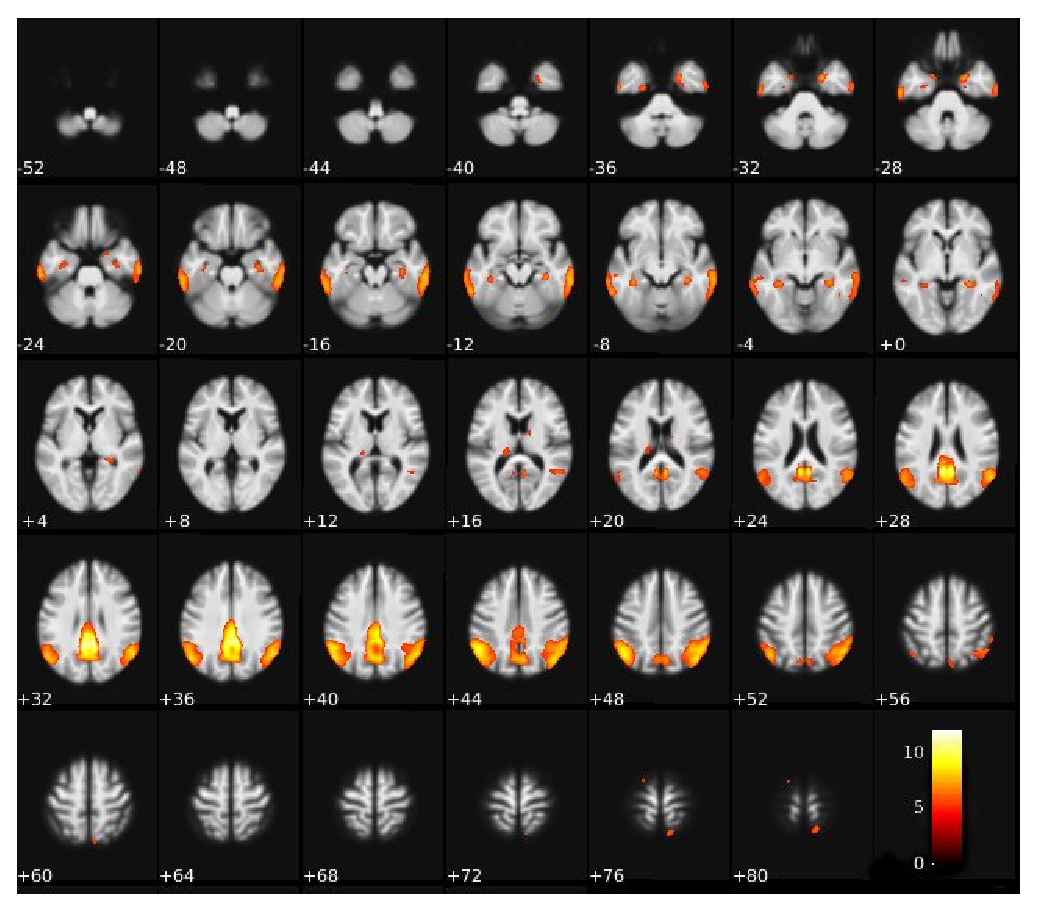
\includegraphics[width=\linewidth]{Graphics/ch2/example_SPM}
	\caption[Example of a \acs{SPM} analysis on a \acs{PET} dataset.]{Example of a \ac{SPM} analysis on a \ac{PET} dataset displaying the differences between \ac{AD} and \ac{CTL}, using $p<0.05$ and \ac{FWE} correction.}
	\label{fig:example_SPM}
\end{figure}

\ac{SPM} outputs maps like the one shown in Figure~\ref{fig:example_SPM}. There, significant $Z$-values according to a given threshold (\ac{FWE} uncorrected or corrected, see Section~\ref{sec:multiplecomparisons}) are displayed over an anatomical reference.  The resulting maps allow a visual inspection of the active brain areas, which can later be related to a certain disease or task. 

Although \ac{SPM}'s main feature is the estimation of differences, the term has been extended to cover the whole process performed by the \ac{SPM} software. That is, it generally involves registration to a template, intensity normalization, smoothing, the proper \ac{SPM} difference estimation and the display of the results. An overview of these procedures is provided at Chapter~\ref{ch:preprocessing}. 

\subsection{Voxel Based Morphometry}
\acf{VBM} can be considered an extention of \ac{SPM} applied to structural \ac{MRI} images \cite{Ashburner2000}. The procedure involves preprocessing (see Chapter~\ref{ch:preprocessing}), where smoothing is applied to reduce smaller anatomical differences. Afterwards, a \ac{GLM} is applied to each voxel in the images, and a $Z$-score map similar to Figure~\ref{fig:example_SPM} is produced. 

Smoothing is more important in \ac{VBM} than in regular \ac{SPM}, since \ac{MRI} images have higher resolution and are less noisy than functional images. Larger smoothing kernels will miss out smaller regions, while smaller kernel can lead to artifacts in the generated $Z$-maps, including misalignment of brain structures, differences in folding patterns or misclassification of tissue types \cite{Martinez-Murcia2016book}. Therefore, the kernel size must be carefully chosen, usually using a-priori knowledge about the regions affected, and always double checking for artifacts and reproducibility. 

The idea behind \ac{VBM} has been extended in a number of papers, using multivariate approaches that takes into account all voxels at once, and not their individual differences. Some of them include \ac{ICA} decomposition of the dataset and a posterior conversion to $Z$-scores in what was called Source Based Morphometry \cite{xu2009source}, or multidimensional Tensor Based Morphometry \cite{bossa2010tensor}. 

\subsection{The Multiple Comparisons Problem}\label{sec:multiplecomparisons}
The Multiple Comparisons problem arises when using hypothesis testing to assess statistical significance. This is widely used in neuroimaging, where statistical tests such as the $t$-Test or \ac{ANOVA} are used to quantify voxel-wise differences, and state their statistical significance, or $p$-value. The $p$-value, as described above, is the probability of any value being more extreme than a certain threshold under a given hypothesis. In our problem, given the $t$-value $T_i$ for the $i^{th}$ voxel ($i=1,\dots N$) of the images, and a threshold $T_{th}$ under the hypothesis $H$, the significance can be assessed by checking:
\begin{equation}\label{eq:pvalue}
P \left(T_i > T_{th}| H_0\right)<\alpha
\end{equation}
where $\alpha$ is the significance level. 

Choosing $\alpha$ is not trivial in neuroimaging. The use of the significance level $\alpha=0.05$ implies that any voxel with a $p$-value smaller than 0.05 is considered sufficient to reject the null hypothesis. This does not directly imply the necessity of accepting the alternative hypothesis $H_1$, although it is often thought so. Neither it yields the probability of the null hypothesis \cite{Dixon2003}. 

If we apply $p<0.05$ directly to a medical image of, for example, 300,000 voxels, that could mean the possibility of almost 15,000 voxels being false positives. Controlling the apparition of false positives when applying a massive univariate test is not trivial. It implies a balance between the true positive rate (sensitivity) or true negative rate (specificity), given that, for example, controlling the amount of false negatives will result in many false positives and vice-versa. 

Usually, two options for controlling the amount of false positives are given: the \acf{FWE} and the \acf{FDR}. The \ac{FWE} is the probability of obtaining at least one type I error. Mathematically, the null hypothesis for the $i^{th}$ voxel $H_{0i}$ states that there is no activation in that voxel. Therefore, the family-wise null hypothesis for our problem is:
\begin{equation}
H_0 = \bigcap_i H_{0i}
\end{equation}

If we reject a single null hypothesis ($T_i > T_{th}$), we reject $H_0$. Therefore, we want to control the probability of a single voxel being significant if the family-wise null hypothesis is valid:
\begin{equation}
P \left(\bigcup_i\{T_i > T_{th}\} | H_0\right)< \alpha
\end{equation}

In this case, we must obtain the critical value $T_{th}$, which is the higher $t$ value that matches that expression. Many options have been proposed to this problem, among them the conservative Bonferroni correction, methods that use random field theory or permutation tests. 

\subsubsection{The Bonferroni Correction}
The Bonferroni correction \cite{Shaffer1995} rewrites eq.~\ref{eq:pvalue} setting $\alpha=\frac{\alpha}{N}$ so that: 

\begin{equation}
P \left(T_i > T_{th}| H_0\right)< \frac{\alpha}{N}
\end{equation}

That way, using the Boole's inequality:
\begin{equation}
FWE \leq \sum_{i}^{N} \frac{\alpha}{N} = \alpha
\end{equation}

Therefore, we can comply with the imposed restriction for a maximum \ac{FWE}, or in our case, a maximum rate $\alpha$ of false positives. This is considered a rather conservative approach. In the example cited above, if we want to keep the \ac{FWE} below $0.05$, we should divide it by $N$, therefore obtaining a $T_{th}$ that makes $\alpha = 0.05/N = 1.67\times10^{-7}$. 

Other less conservative options try to compute a critical value $T_{th}$ that minimizes the \ac{FWE} using spatial information. This is the case of using an approximation of the distribution of the maximum statistic over the image, or the spatial correlation, including elements from random field theory (the approach used in \ac{SPM} \cite{spm_book}). 

\subsubsection{Random Field Theory}
In the random field approach, the maps of the statistic are treated, under the null hypothesis, as a lattice representation of smooth isotropic three dimensional random fields of test statistics. This approximation to the problem allow us to approximate the upper tail of the maximum distribution, the part needed for defining an event that occurs when the map exceeds the critical value $T_{th}$. Further information about random field theory and how it is applied to neuroimaging can be found at \cite{spm_book}. 

The other approach, based on the \ac{FDR}, aims at controlling the proportion of false positives in the total number of voxels declared significant. The most extended procedure for controlling the \ac{FDR} is that proposed by Benjamini and Hochberg \cite{Benjamini1995}. The Benjamini and Hochberg method start with calculating the $p$-values of all voxels and ranking them so that:
\begin{equation}
p_1 \leq p_2 \leq \dots \leq p_i \leq \dots \leq p_N \quad \forall i=1\dots N
\end{equation}

\subsubsection{FDR Controlling Procedures}
Let $q$ be the a maximum \ac{FDR} value that we can afford, for example $0.05$. For each $i$, we compute:
\begin{equation}\label{eq:bhFDRineq}
p_i \leq \frac{i}{N}q
\end{equation}

The maximum $i$ value that holds Eq.~\ref{eq:bhFDRineq} is used as $\alpha$, the significance level, and its corresponding statistical value ($T_i$ in the case of a $t$-test) is used as the critical value. This test, under the family-wise null hypothesis $H_0$, is equivalent to controlling the \ac{FWE}. However, \ac{FDR} methods are less conservative than other approaches such as the Bonferroni or other \ac{FWE}-based corrections, leading to a gain in statistical power. 


\subsubsection{Permutation Tests}
An empirical way to obtain $p$-values without relying on any parametric assumption is permutation testing \cite{Anderson2001,Winkler2014}. Permutation tests evaluate a statistic such as the F-statistic or the $t$-test using randomly target variables, in our case, the classes. The procedure is applied many times (up to 10,000), and for each permutation, only the maximum value of the computed statistic is considered. These values are used to build the null distribution, from which the family-wise corrected $p$-values are computed. Results obtained in permutation tests are comparable to those obtained using Random Field Theory \cite{Winkler2014}, and far less conservative than when applying the Bonferroni correction. 

\section{Machine Learning in Neuroimaging}\label{sec:machinelearning}
Machine learning is a current trend in neuroimaging. It provides computers with the ability to learn from data, using a set of statistical and computational tools. Rather than being explicitly programmed for a certain task, machine learning systems are able to find relevant data, discover patterns and predict the outcome of the input data. Its application to medicine is often known as \acf{CAD} \cite{Martinez-Murcia2016}. 

There are two major branches of machine learning: supervised and unsupervised learning. Th former explores the patterns that lead to a certain outcome, whereas on the other hand, unsupervised learning explores the underlying structure of the data. Most of the \ac{CAD} systems rely on supervised learning, since their intention is to discover patterns that can effectively predict a disease. 

\begin{figure}[htp]
	\centering
	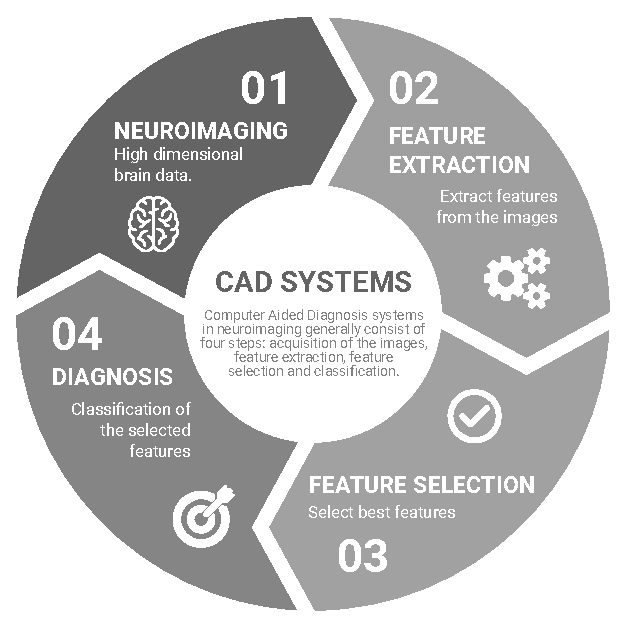
\includegraphics[width=0.5\linewidth]{Graphics/ch2/NI-CAD}
	\caption[Illustration of a typical neuroimaging CAD system.]{Illustration of a typical neuroimaging CAD system.}
	\label{fig:ni-cad}
\end{figure}

For simplicity, in this thesis, when talking about \ac{CAD}, we will always refer to automatic \ac{CAD} systems. That is, those that, once trained with previously known data, can predict the outcome of new, unseen data. A typical \ac{CAD} system, like the one in Figure~\ref{fig:ni-cad}, consists of input data (in our case, neuroimaging), feature extraction, feature selection and a classification step. The most basic is the \acf{VAF} approach, in which all voxels are considered as features, and then used as input to the classifier \cite{Stoeckel04}. However, many more advances can be made in this field by exploring different types of 

\subsection{Voxels as Features}
\acf{VAF} \cite{Stoeckel04} is an example of the simplest \ac{CAD} system. It was originally proposed for evaluating and performing automatic diagnosis of \ac{AD} using functional \ac{SPECT} imaging. It uses a standard preprocessing (registration, intensity normalization) and a \ac{SVC} (See Appendix~\ref{ch:svm}) to predict the class of an image using all its intensities as features. Feature extraction, here, considers all voxels, and then there is no feature selection applied. 

It has been used in many works as a baseline \cite{Spetsieris2009,Salas-Gonzalez2009,Martinez-Murcia2016}, since it is comparable to the performance achieved by expert physicians using visual analysis \cite{Stoeckel04}. The weight vector of the \ac{SVC} can be inverse transformed to the dimension of the original images, and therefore provide a visual map that reflects the most influential voxels, in a similar way to the $Z$-maps of \ac{SPM} and \ac{VBM}. 

\subsection{Multivariate Analyses}\label{sec:mvanalyses}
Many improvements can be made to \ac{VAF} by adding and refining feature extraction and feature selection techniques. With this addition, we can avoid the Small Sample Size, in addition to the ability to discover higher level abstractions that can be more representative of the progression of the studied diseases. 

Feature extraction algorithms often change the strategy from a massive univariate approach, where a single feature is considered at each time, to multivariate analyses, where each feature can contain information from many voxels at the same time. Measures of total uptake of a given drug in nuclear imaging are a good example of this \cite{Zhou2007,Lozano2007}, but also the widespread Cortical Thickness \cite{Dale1999} provided by \textit{FreeSurfer}. Cortical thickness is an estimation of the amount of \ac{GM} in a direction perpendicular to its surface. It first estimates the \ac{GM}-\ac{WM} and the \ac{WM}-\ac{CSF} separation surfaces, and then characterizes the thickness of the tissue, allowing a characterization of \ac{GM} differences such as atrophy or hypetrophy. Other pieces of software, such as \ac{SPM}, also include toolboxes to compute cortical thickness, providing outputs such as the one that can be seen in Figure~\ref{fig:corticalthickness}. 

\begin{figure}
\centering
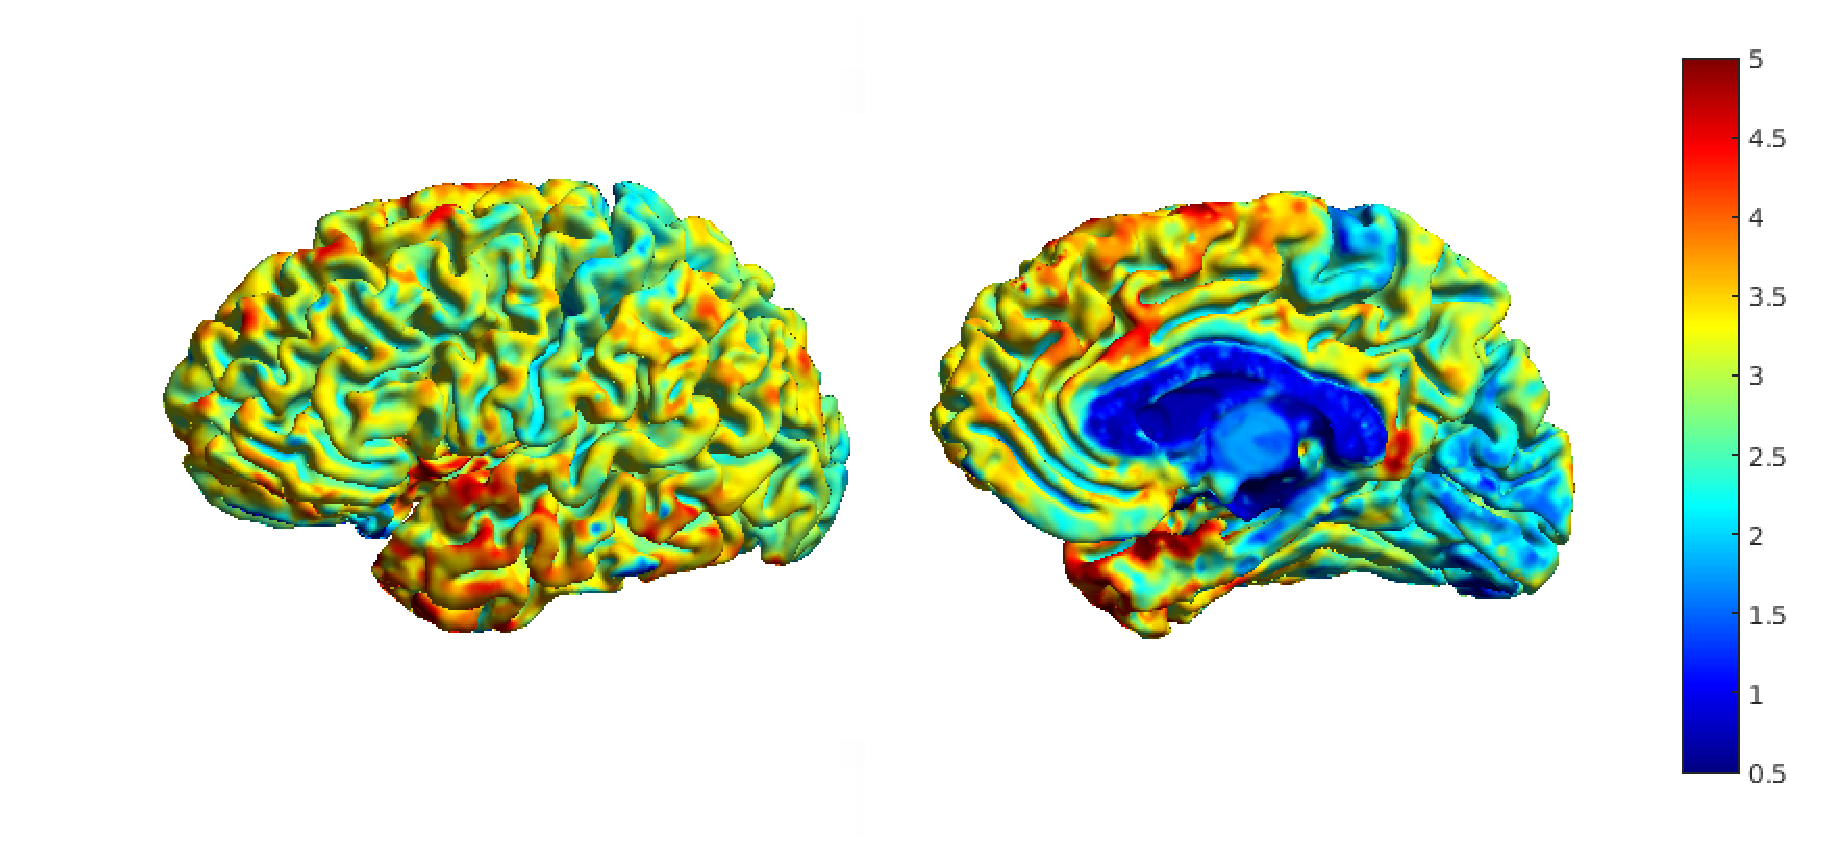
\includegraphics[width=0.8\linewidth]{Graphics/ch2/corticalThickness}
\caption[Example of the cortical thickness of a subject.]{Example of the cortical thickness of a subject, obtained with the toolbox CAT12 in SPM12.}
\label{fig:corticalthickness}
\end{figure}

Other more advanced algorithms are image decomposition techniques such as \ac{PCA} or \ac{PLS}, which have been extensively used in neuroimaging \ac{CAD} systems \cite{Spetsieris2009,Illan2011,Towey2011,Segovia2013,Khedher2015}. In these approaches, a given image can be represented as the linear combination of different components, and while the component loadings are common to all subjects, the weights of these components are unique to each patient. This allows us to identify the patterns that better discriminate between classes, leading to a more accurate diagnosis. 

For its part, feature selection refers to different strategies aimed at finding an optimal subset of the extracted features, according to a certain criterion. Irrelevant features are therefore discarded, making our models faster and more cost-effective \cite{Guyon03}. Feature selection algorithms are often subdivided in three approaches \cite{Martinez-Murcia2016b}: filters, wrappers and embedded approaches. 

Filters compute a feature relevance score from the data, which is then used to sort the different features. It is computed before the classification, and does not interact with it. Many scores can be derived from statistical features such as $\chi^2$, $t$-Test, Fisher's Discriminant Ratio (FDR) or others \cite{Martinez-Murcia2013255,Martinez-Murcia2016b}. The output of these tests has been already used as a tool in voxelwise analyses, as we commented in Section~\ref{sec:vwanalyses}. 

Wrappers are similar to filtering methods, given that they assign a certain score to each feature. But in contrast to filters, the score is computed by estimating the performance in a predictive model, such as classifiers \cite{Kohavi1995}. The most obvious measure here is accuracy, although other techniques such as Forward selection, backward elimination \cite{Guyon03}, genetic algorithms  \cite{Kohavi1995}, or the expectation-maximization algorithm \cite{Gorriz2009} have been used in the literature. And finally, embedded approaches use the very model that is being built to construct their optimal feature subset. 

%************************************************
%\chapter{Image Preprocessing}\label{ch:preprocessing} % 
\chapter{General Methodology}\label{ch:preprocessing} % $\mathbb{ZNR}$
%************************************************
To perform most automated analyses on neuroimaging, it is fundamental that images are comparable. Preprocessing comprises a series of algorithms that, applied after the acquisition and reconstruction of the images, produce directly comparable images in both structure and magnitude. 

In this section we present the preprocessing algorithms used in this thesis. Whether they have been used in one or all experiments, they can be classified in two major categories: spatial and intensity preprocessing. Later, in Section~\ref{sec:vwanalyses}, we present some voxelwise analyses, commonly used in clinical practice, that we have set as a baseline in our experiments. 

\section{Spatial Preprocessing }
Spatial processing usually accounts for the differences in position, angles and structure that are commonly found between images. A common pipeline in, for example, \ac{MRI} preprocessing, is the one found at Figure~\ref{fig:examplePreMRI}, where the images are registered (or spatially normalized) to a template, smoothed and finally segmented. The smoothing is an optional step, generally used in procedures like segmentation or \ac{VBM}. 

\begin{figure}[htp]
	\myfloatalign
	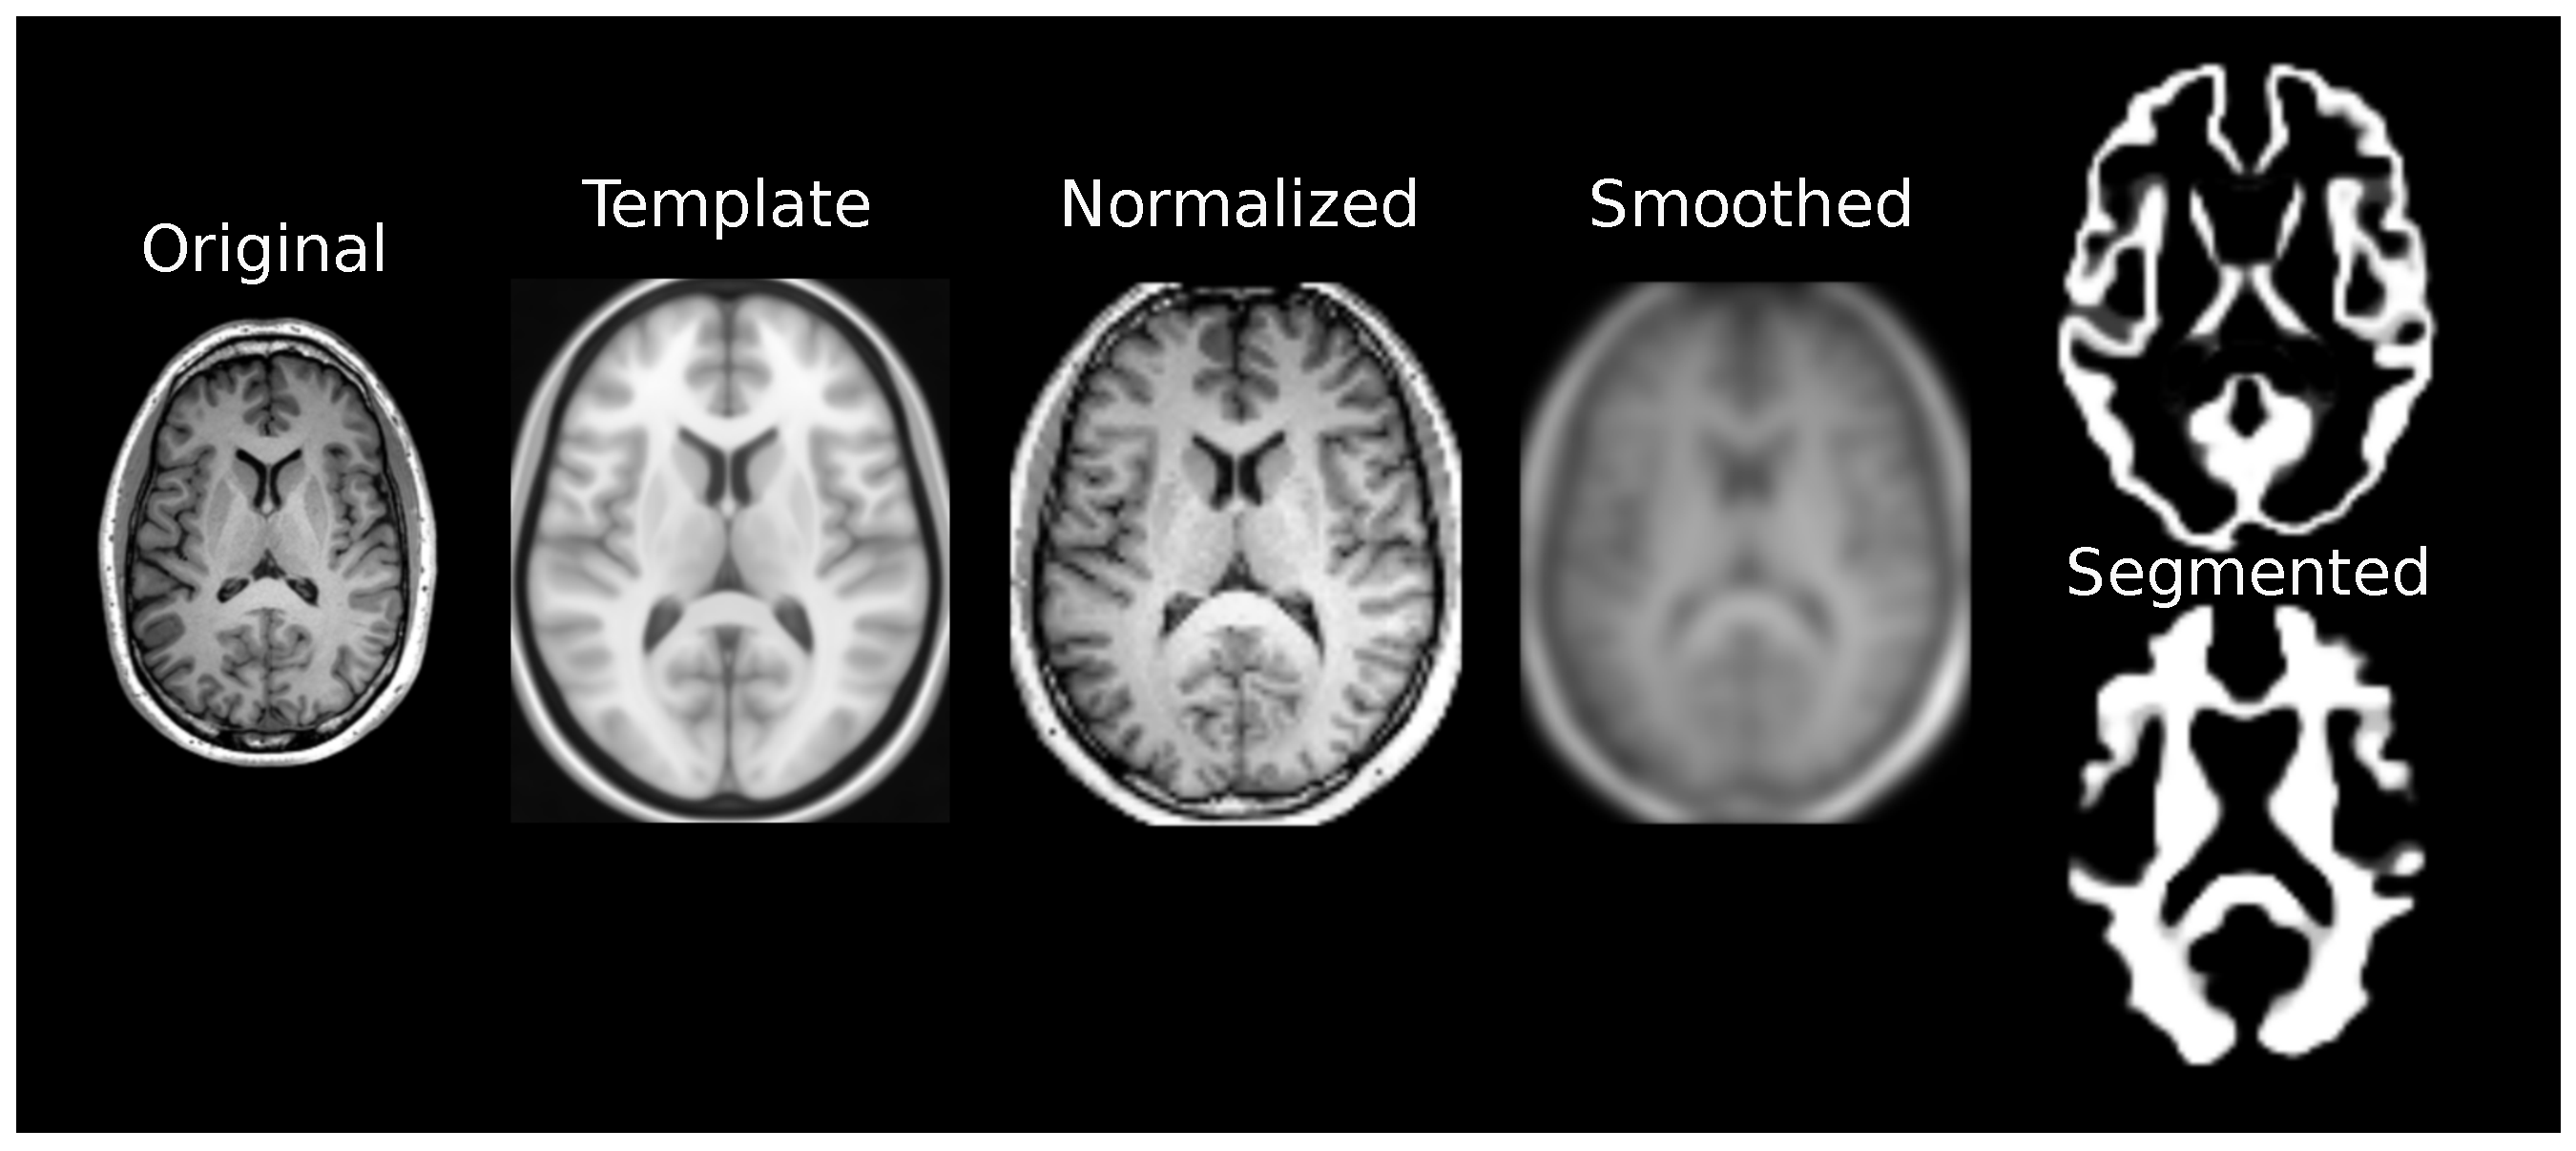
\includegraphics[width=.75\linewidth]{Graphics/ch3/preProcessPL}
	\caption[Typical pre-processing pipeline in MRI]{Typical pre-processing pipeline in \ac{MRI}.}\label{fig:examplePreMRI}
\end{figure}

In this thesis, all the experiments in all image modalities involve spatial normalization. Smoothing, as well as segmentation, is only applied in some experiments that use \ac{MRI} images, such as the segmented images in Chapter~\ref{ch:sbm} or the whole-brain analysis performed in Chapter~\ref{ch:swpca}. 

\subsection{Spatial Normalization or Registration}
Spatial Normalization, also known as Registration, is the procedure that by which every subject's brain is mapped from their individual space to a standard reference system. Registered images allows our system to overcome the individual differences in position and anatomy by establishing a common reference space in which a given coordinate represent the same anatomical position in all brains in the dataset. 

There exist a number of pieces of software widely used for registering images, such as FreeSurfer \cite{Reuter2010} or FSL (in the FLIRT and FNIRT package) \cite{Smith2004}, most of them perform linear, non-rigid and elastic transformations or a combination of these. In this work we have used the software SPM8 \cite{spm_book} to perform registration of all the datasets, including \ac{MRI}, \ac{SPECT} and \ac{PET} images. So, from this moment, we will focus on the registration as performed in the \ac{SPM8}. 

Linear registration usually refers to the affine transformation, a matrix multiplication that includes 12 parameters for translation, rotation, scale, squeeze, shear and others: 
\begin{equation}\label{eq:affine}
	\left[\begin{matrix}
	x'\\y'\\z'\\1
	\end{matrix}\right]
	 = \left[\begin{matrix}
	 a_{00} & a_{01} & a_{02} & a_{03}\\
	 a_{10} & a_{11} & a_{12} & a_{13}\\
	 a_{20} & a_{21} & a_{22} & a_{23}\\
	 0 & 0 & 0 & 1\\
	 \end{matrix}\right]
	 \left[\begin{matrix}
	 x\\y\\z\\1
	 \end{matrix}\right]
\end{equation}

This matrix multiplication is performed globally, as it transforms the whole image, not accounting for local geometric differences. In equations \ref{eq:affine1}, \ref{eq:affine2} and \ref{eq:affine3} we give an example of the parameters that are computed for scale, translation and shear in 3D:

\begin{align}
\label{eq:affine1}
	\text{scale} &= 
	\left[\begin{matrix}
		 s_x  &0 & 0 & 0\\
		0 &s_y &0 &0\\
		0 &0 &s_z &0\\
		0 &0 &0 &1		
	\end{matrix}
	\right]\\
	\label{eq:affine2}
	\text{translation} &= 
	\left[
	\begin{matrix}
	1  &0 & 0 & \Delta x\\
	0 &1 &0 &\Delta y\\
	0 &0 &1 &\Delta z\\
	0 &0 &0 &1		
	\end{matrix}
	\right] \\
	\label{eq:affine3}
	\text{shear} &= 
	\left[\begin{matrix}
	1  &h_{xy}& h_{xz} & 0\\
	h_{yx} &1 &h_{yz} &0\\
	h_{zx} &h_{zy} &1 &0\\
	0 &0 &0 &1		
	\end{matrix}
	\right]
\end{align}

The combination of all these operations result in the estimation of the twelve parameters that we found in Eq.~\ref{eq:affine}, which are the ones used in \ac{SPM8}. The estimation of these parameters is performed via the optimization of a cost function, that in \ac{SPM8} can be the minimum squared difference between the source image and the template \cite{spm_book} in the case of within-modality registration, or the mutual information in between-modality registration. These functions are also used in FLIRT \cite{Jenkinson2001}, whereas FreeSurfer uses the Tukey's biweight function (in {\ttfamily mri\_robust\_template}) \cite{Reuter2012}.

After the affine transform, the software usually performs a fine-tuning step via nonrigid transformations, to account for relevant a\-na\-to\-mi\-cal differences between subjects. Nonrigid transformations range from the use of radial basis functions, physical continuum models and the large deformation models, or diffeomorphisms, that \ac{SPM8} uses. These procedures work by estimating a warp-field and then, apply it to the affine-registered images. An example of the differences of using only affine registration and applying diffeomorphisms can be found at Figure~\ref{fig:diffeomorphisms}.

\begin{figure}[bth]
	\myfloatalign
	\subfloat[Comparison in \ac{MRI}.]
	{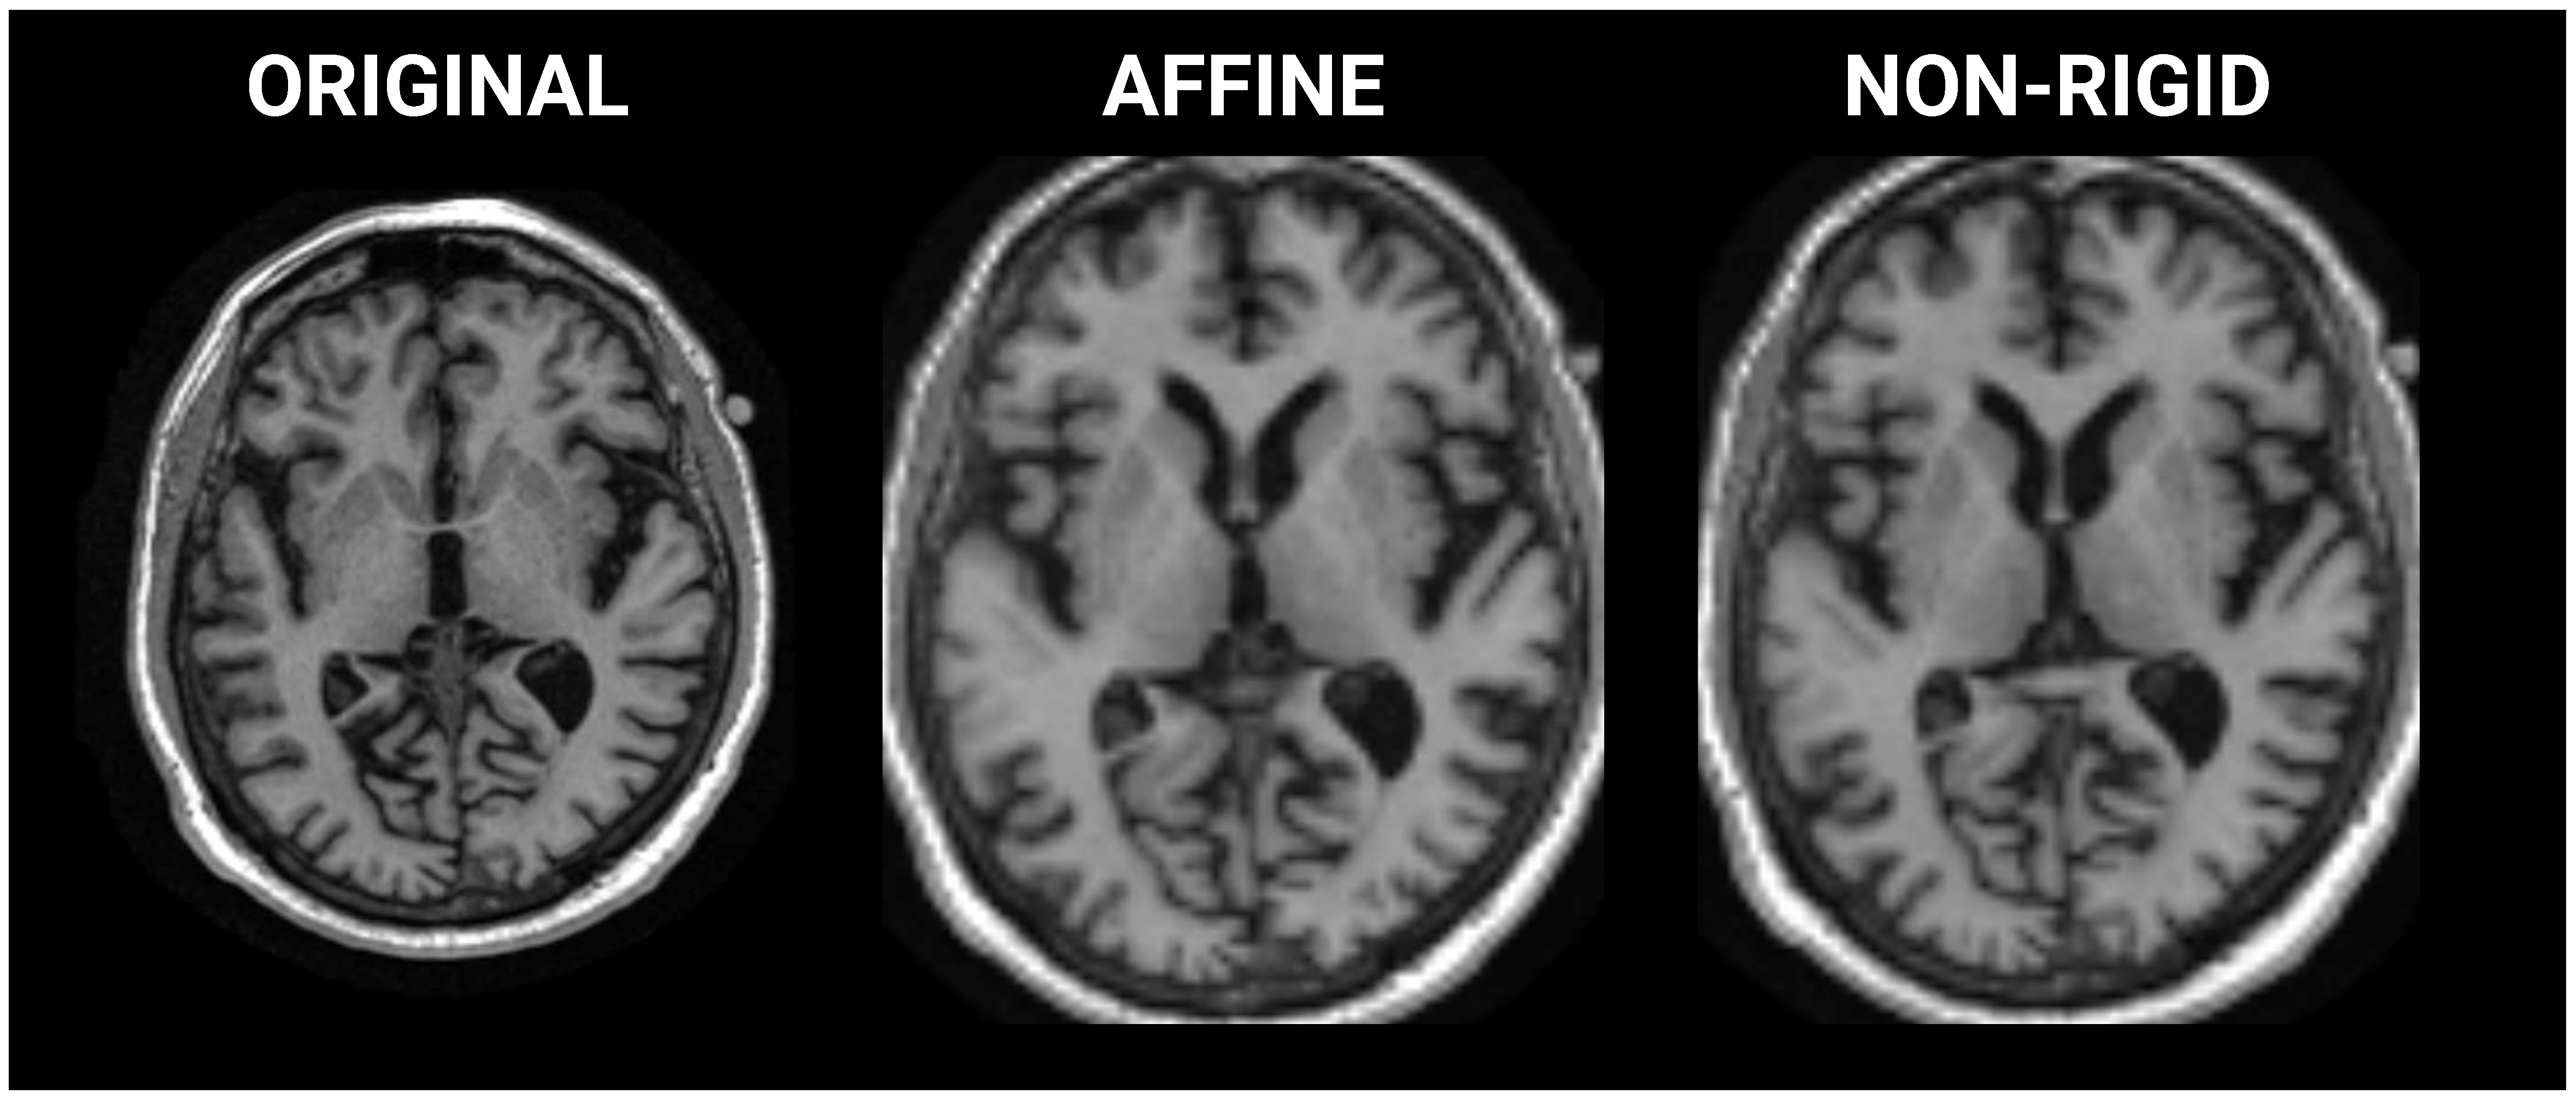
\includegraphics[width=.7\linewidth]{Graphics/ch3/regComparisonMRI}}
	 \\
	\subfloat[Comparison in \ac{PET}.]
	{\includegraphics[width=.7\linewidth]{Graphics/ch3/regComparisonPET}}
	\caption[Comparison of the affine registration and the application of non-linear transformations to the images]{Comparison of the affine registration and the application of non-linear transformations to both \ac{MRI} and \ac{PET} images of the same \ac{ADNI} subject.}\label{fig:diffeomorphisms}
\end{figure}


\subsubsection{Co-registration}
Sometimes we have several image modalities of the same subject, for example \ac{MRI} and \ac{PET} or functional \ac{MRI}, often acquired at the same time. In this particular case, we can use the higher resolution \ac{MRI} image to calculate the affine parameters and warping, and apply those to all modalities of the same subject. To do so, we perform a first co-registration, that is, a registration of the lower-resolution images (e.g. \ac{PET}) to its correspondent \ac{MRI} image. Being anatomically similar, the co-registration usually comprises a single affine transformation. Afterwards, we can proceed with the registration of that \ac{MRI} image to the template, and apply the same transformation to all its co-registered images. 

\subsubsection{The MNI Space}
In this thesis, all images are coregistered to the \acf{MNI} space \cite{Mazziotta2001}. This is the most widely used coordinate system, recently adopted by the International Consortium for Brain Mapping (ICBM) as its standard template. The three-dimensional coordinate system defined in \ac{MNI} was intended to replace the Tailarach space, a system based on a dissected brain, that was used to compose an atlas by Tailarach and Tournoux \cite{Talairach1988c}. The current template is known as ICBM152, and features the average of 152 normal \ac{MRI} scans matched to an older \ac{MNI} template using a nine parameter affine registration. 

\subsection{Segmentation}
When using \ac{MRI} images in this thesis, we often refer to \acf{GM} and \acf{WM} maps, which is the result of the segmentation of the original data. Segmentation aims at producing maps of the distribution of different tissues, and it generally addresses \ac{GM}, \ac{WM} and \ac{CSF} classes, although lately some software can output data for bone, soft tissue or very detailed functional regions and subregions \cite{Fischl2002}. 

In this thesis we have used the \ac{VBM} toolbox of the \ac{SPM8} software, which yields \ac{GM}, \ac{WM} and \ac{CSF} maps. It features an \ac{EM} algorithm to model the distribution of the tissue classes as a mixture of gaussians and, by combining this distribution-based information with tissue probability maps using a bayesian rule, the software produces joint posterior probability maps for each tissue. To clean up the segmentation maps, a series of iterative dilations and erosions are used. Finally, since brain regions are expanded or contracted at the spatial normalization step, we can scale the segmented maps using modulation, producing final maps where the total amount of grey matter is preserved. 

\section{Intensity Normalization}
Generally, structural modalities such as T1 and T2-weighted images are considered unitless, in contrast to functional imaging, in which each voxel's intensity represent the distribution of some biomarker, such as glucose metabolism, dopamine transporters, etc. These amounts are affected by many sources of variability that can affect the final values: contrast uptake, radiotracer decay time, metabolism, etc. Therefore, along with the previous spatial normalization, there is a need to normalize the intensities of the images, so that the amount they represent are comparable. 

In the case of intensity normalization, the method acts as a linear transformation of the image, preserving fundamental information such as contrast between regions. This approximation estimates the new intensity values $I'$ as: 
\begin{equation}
	I' = I/I_p 
\end{equation}
where $I_p$ is a constant parameter that is unique for each image. After this division, the new intensities would be directly comparable. The technique used to compute the normalization parameter varies, ranging from the simplest normalization to the maximum \cite{Salas-Gonzalez2009,Martinez-Murcia20129676} to complex methodologies that use assumptions about the image's \ac{PDF}. 

The \emph{normalization to the maximum} strategy computes $I_p$ as the average value of the 95th bin of the histogram of the image. In other words, this mean averaging the 5\% higher intensity values and use this mean as $I_p$. Another useful approach is the so-called \emph{integral normalization}, which computes $I_p$ as the sum of all values in the image. 

Other approaches involves some a-priori knowledge about the intensity distribution of normal subjects in a certain modality. This is the case of setting $I_p$ to the Binding Potential (BP), a ratio between the intensities at specific and non-specific areas \cite{Scherfler2005}. 

Finally, more advanced approaches use a general linear transformation of the image: 
\begin{equation}
	I' = a I + b
\end{equation}
The parameters $a$ and $b$ are so that the \ac{PDF} of a given matches a reference \ac{PDF}. There exist methods that use the histogram \cite{Arndt1996}, the gaussian distribution or the alpha-stable distribution \cite{Salas-Gonzalez2013}. In this latter case, the parameters $a$ y $b$ are computed as linear transformations of some distribution's parameters: 
\begin{equation}
	a = \frac{\gamma*}{\gamma}, \quad b = \mu* + \frac{\gamma*}{\gamma} \mu
\end{equation}
where $\gamma*$ and $\gamma$ are the dispersion parameters of the alpha-stable intensity distribution of the non-normalized and the reference image respectively, and $\mu*$ and $\mu$ are the location parameters of the same images. 

Despite traditionally structural modalities such as \ac{MRI} did not use intensity normalization, there exist a new tendency towards the use of \ac{qT1} and \ac{qT2} images \cite{Weiskopf2013} that provide biomarkers for absolute measures such as myelination, water and iron levels. This strategy is especially designed to overcome different sources of variability that affect multicentre studies, e.g. magnetic field inhomogeneity, noise, evolution of the scanners, etc. The role of those in multi-centre studies is addressed at Chapter~\ref{ch:swpca}. 

See Figure~\ref{fig:comparisonIntNorm} for a comparison between different strategies of intensity normalization on the same images. 

\begin{figure}[bth]
	\myfloatalign
	\subfloat[Normalization to the Maximum.]
	{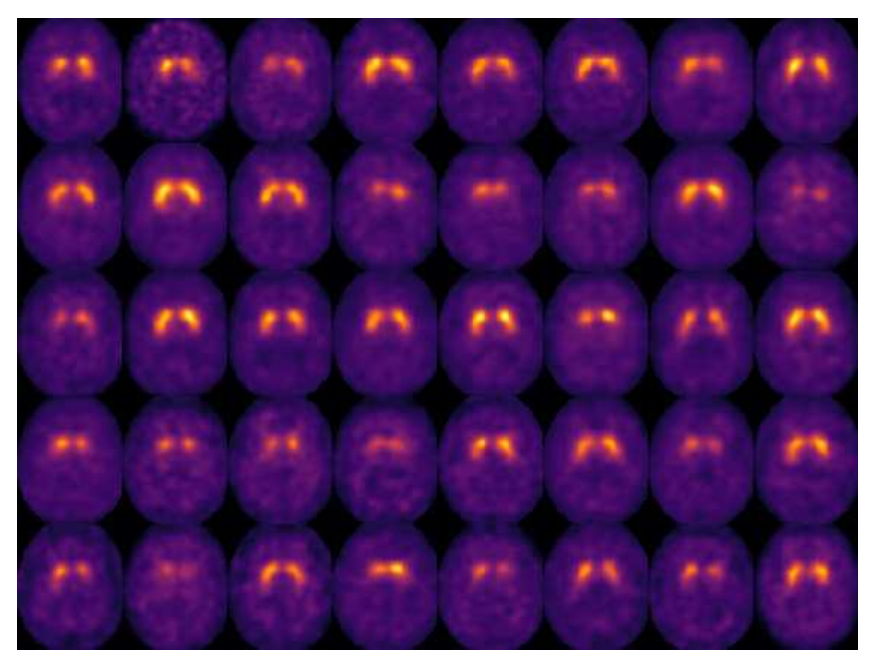
\includegraphics[width=.45\linewidth]{Graphics/ch3/norm_max.eps}}\quad
	\subfloat[Integral Normalization.]
	{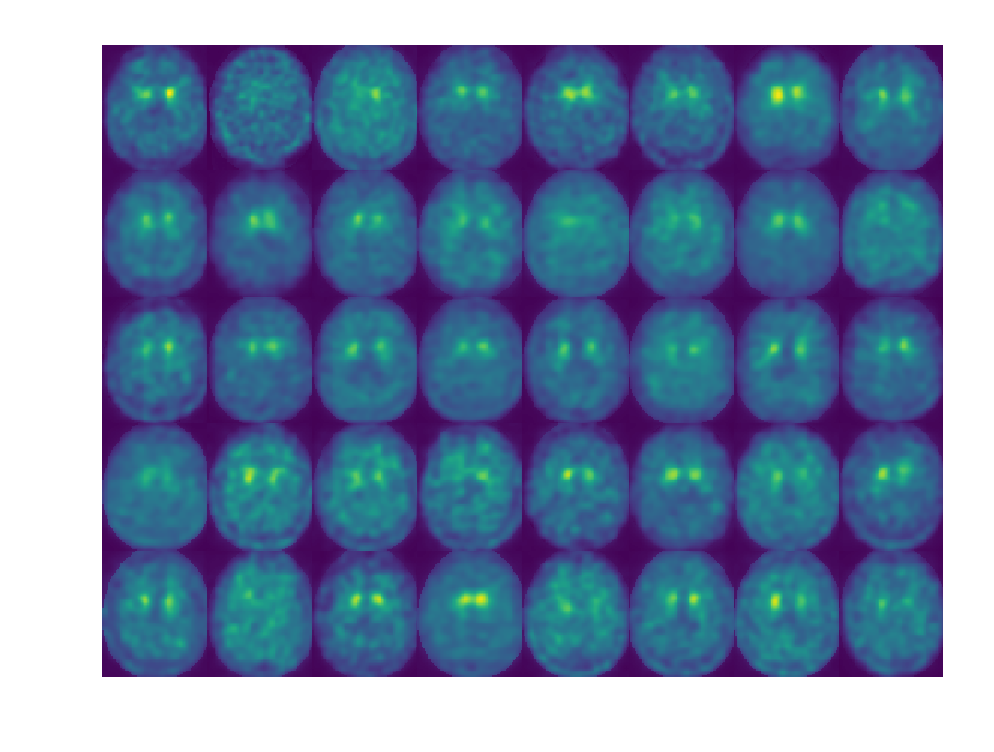
\includegraphics[width=.45\linewidth]{Graphics/ch3/norm_int.eps}}\\
	\subfloat[Normalization using $\alpha$-stable distribution.]
	{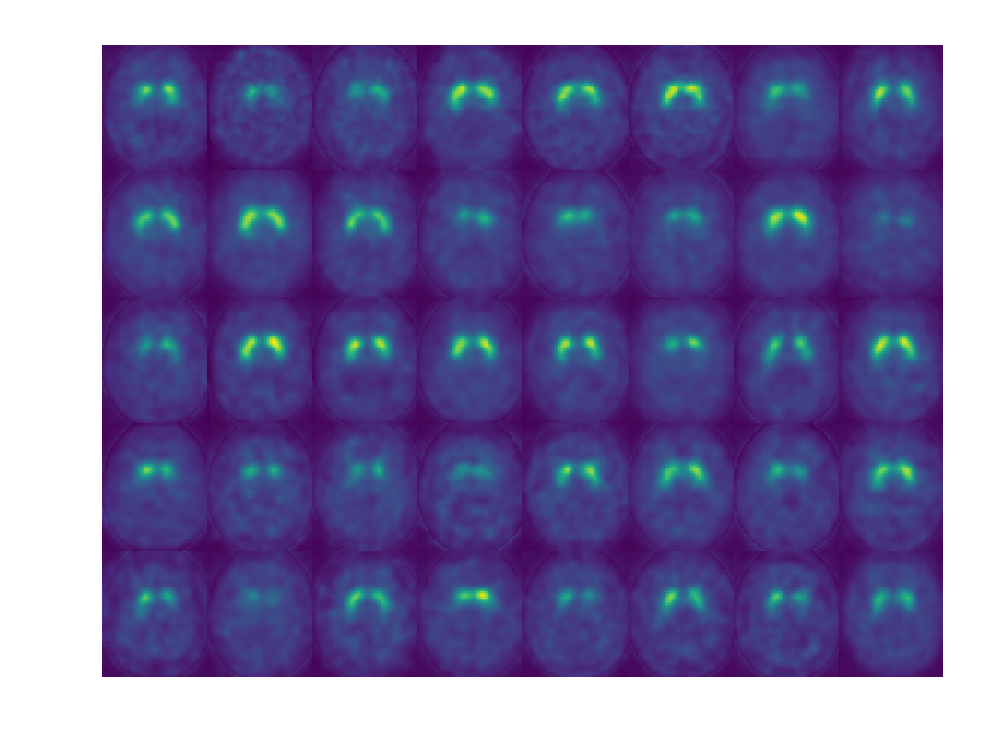
\includegraphics[width=.45\linewidth]{Graphics/ch3/norm_est.eps}}
	\caption{Comparison between different types of intensity normalization, applied to the VDLN-DAT dataset (see Appendix~\ref{ch:datasets}).}\label{fig:comparisonIntNorm}
\end{figure}
%DONE


\section{Evaluation Parameters and Methodology}\label{sec:validation}
\subsection{Cross-validation}

The classification was validated using stratified 10-fold
cross-validation (Kohavi, 1995). In brief, 9 subsets of the dataset
were used for extraction of the PCs and training of the classifier with
the remaining subset used for testing. This procedure was repeated for
each subset, repeated 10 times to avoid possible bias and random
effects of the partitions. The average and standard deviation of the
accuracy (acc), sensitivity (sens) and specificity (spec) values for
each repetition were recorded. 

\subsection{Classification Performance}

The proposed methodology has been tested on the three previously described databases, using a cross-validation method called leave-one-out to extract several performance parameters: accuracy, sensitivity, specificity, positive likelihood (PL) and negative likelihood (NL). This method achieves an almost unbiased error estimate, however it might be affected by the database topology, reason why we used different databases to test our method.

Along with the widely used sensitivity, specificity and accuracy (which are prevalence dependent), we use the Positive and Negative Likelihood ratios (PL and NL) to provide some prevalence independent parameters that are also widely used in clinical medicine, where values of PL greater than 5 or NL values less than 0.2 can be applied to the pre-test probability of a patient having the disease tested for to estimate a post-test probability of the disease state existing \cite{McGee2002}. A positive result for a test with an PL of 8 adds approximately 40\% to the pre-test probability that a patient has a specific diagnosis. 

To provide a better understanding of the accuracy distribution (mean, range, skewness), we have made use of the box plot (Fig. \ref{fig:features_acc_distances}). In these plots, the median for each group of data is indicated by the red center line, and the first and third quartiles are the edges of the blue box, which is known as the inter-quartile range (IQR). The extreme values (within 1.5 times the inter-quartile range from the upper or lower quartile) are the ends of the lines extending from the IQR. Points at a greater distance from the median than 1.5 times the IQR are plotted individually, representing potential outliers. 




\cleardoublepage
\ctparttext{The first approach to reduce the small sample size problem in neuroimaging studies is based on reducing the number of features .}
\part{Reducing the Feature Space}
%\addtocontents{toc}{\protect\clearpage} % <--- just debug stuff, ignore
%************************************************
\chapter{Image Decomposition}\label{ch:decomposition}
%************************************************

In this chapter, we will focus on those \ac{CAD} systems that use a combination of an image decomposition method and feature selection by means of hypothesis testing. These variety of methods have been published in \cite{Martinez201141,Martinez-Murcia20129676,Martinez-Murcia2013255,Martinez-Murcia201458}. 

Image decomposition methods model a set of samples as a linear combination of $c$ latent variables, also known as components. These variables can be considered as the basis of a $c$-dimensional space where each sample is represented by a feature vector of length $c$. The $i$-th neuroimage in our dataset can be therefore decomposed as: 

\begin{equation}\label{eq:generalDecomposition}
	\mathbf{x}_i = s_0 \mathbf{w}_0 + s_1 \mathbf{w}_1 + \dots + s_c \mathbf{w}_c + \boldmath\epsilon = \mathbf{s}\mathbf{W} + \boldmath\epsilon
\end{equation}

Where $s_i$ is the coordinate (or component score) of the current image in the $i$-th dimension of the new space defined by all the base vectors $\mathbf{w}_i$ (component loadings), and $\boldmath\epsilon$ is the error of the estimation. Figure \ref{fig:decomposition_overview} shows an illustration of the process. 

\begin{figure}[tph]
	\centering
	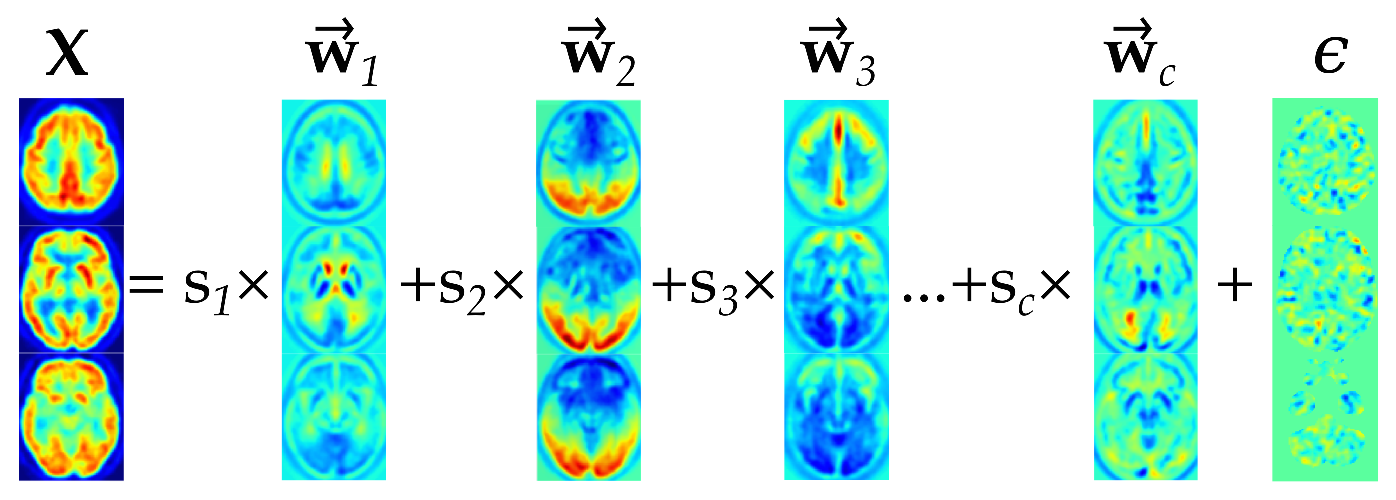
\includegraphics[width=0.9\linewidth]{Graphics/ch4/decomposition_overview}
	\caption[Illustration of how decomposition algorithms work.]{Illustration of how decomposition algorithms such as \ac{FA} and \ac{ICA} work on a \ac{PET}-FDG brain image.}
	\label{fig:decomposition_overview}
\end{figure}

Many signal decomposition techniques are used in the literature, for example \ac{PCA} or \ac{PLS} \cite{Spetsieris2009,Illan2011,Towey2011,Segovia2013,Khedher2015}. We will focus on two less known decomposition algorithms \acf{FA} and \acf{ICA}, which we will integrate in different \ac{CAD} systems using a pipeline similar to the one displayed at Figure~\ref{fig:pipelineDecomposition}. This pipeline involves feature selection (for reducing the dimensionality), decomposition of the feature vectors and classification.
 
\begin{figure}[tph]
	\centering
	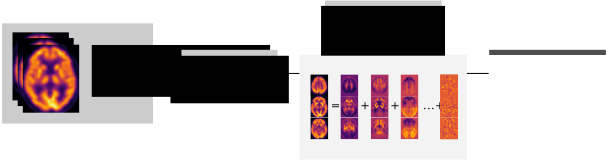
\includegraphics[width=0.7\linewidth]{Graphics/ch4/01-flowdiagram}
	\caption[Illustration of the system used in Chapter~\protect\ref{ch:decomposition} .]{Illustration of the system used in Chapter~\protect\ref{ch:decomposition}.}
	\label{fig:pipelineDecomposition}
\end{figure}

\section{Feature Selection}
Feature selection is the first strategy used for feature reduction \cite{Martinez-Murcia2016b}, and it is often used along with feature extraction in order to build more complex pattern recognition systems. It refers to any strategy intended to find a subset of the original features containing the more suitable ones according to a certain criterion. Therefore, irrelevant features are discarded, and resultant models are faster and more cost-effective \cite{Guyon03}. However, it usually requires an additional optimization to find the parameters for the optimal feature subset, and furthermore, it is impossible to guarantee that the optimal features for the subset are the same of the full feature set \cite{DaelemansHosteMeulderEtAl2003}. 

In this work, we will use filtering methods to perform feature selection. As we introduced in Section~\ref{sec:mvanalyses}, filtering methods are based on the computation of a feature relevance score directly on the data. The relevance score is used to sort the different features, discarding those with a lower score, and it is usually computed independently for each feature, in what is called a univariate approach \cite{SaeysInzaLarranaga2007}. 

Feature selection can be used before or after feature extraction. When using computationally-intensive algorithms such as \ac{FA} or especially \ac{ICA}, the selection of best features prior to the decomposition is key to obtain high performance while keeping the computation times small \cite{Martinez201141,Martinez-Murcia20129676}. This also removes noise in some cases where the decomposition algorithm cannot compute correctly the variance. 

\begin{figure}[bth]
	\myfloatalign
	\subfloat[$t$-test.]
	{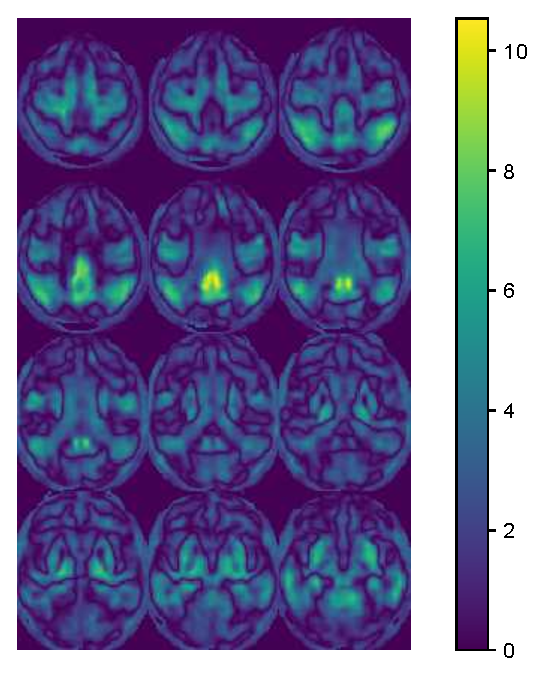
\includegraphics[width=.3\linewidth]{Graphics/ch4/ttest_map.eps}\label{fig:ttest_map}}\quad
	\subfloat[\ac{KL} divergence.]
	{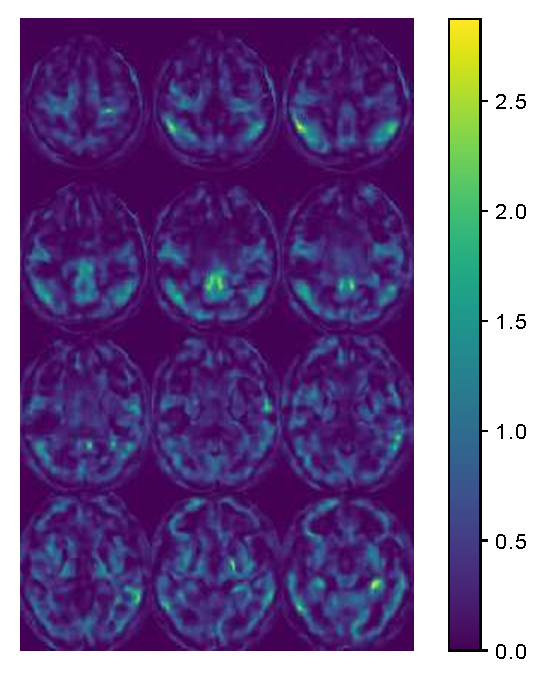
\includegraphics[width=.3\linewidth]{Graphics/ch4/kl_map.eps}\label{fig:kl_map}}\quad
	\subfloat[\ac{MWW} $U$-test.]
	{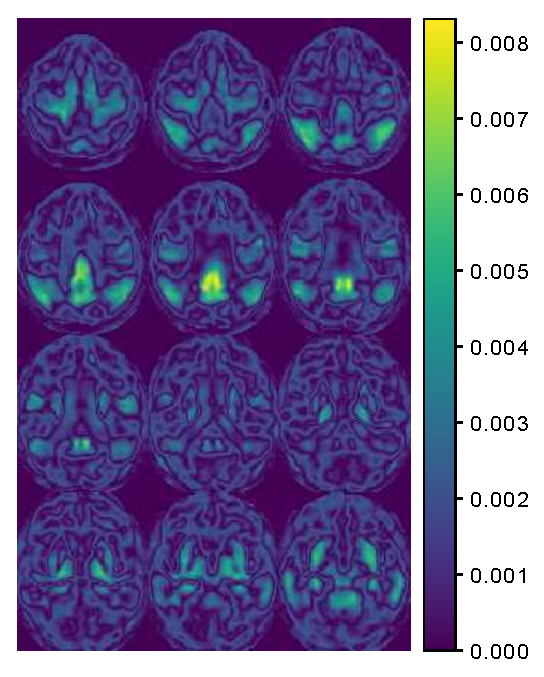
\includegraphics[width=.3\linewidth]{Graphics/ch4/wilcoxon_map.eps}\label{fig:wilcoxon_map}}
	\caption[Comparison between the different filtering methods.]{Comparison between the different filtering methods, and the regions selected by them, in the ADNI-PET dataset. }\label{fig:comparisonSelection}
\end{figure}

Three feature selection algorithms have been used in this thesis, not only in the \ac{CAD} systems proposed in this chapter, but in many other models that will be presented later: the $t$-Test, the Kullback-Leibler divergence or Relative Entropy, and the Mann-Whitney-Wilcoxon rank test. 

\subsection{$t$-test}
The $t$-test is an old friend of statisticians. In this work we will use the independent two-sample $t$-test \cite{Fay10}. It quantifies the differences between two classes using an assumption of independent variances. Let $X_i^f$ a vector containing the $f$-th feature of all elements in class $i$. The $t$-score of the $f$-th feature can be computed as:

\begin{equation}
t_f = \frac{\bar{X}_1^f - \bar{X}_2^f}{\sqrt{\frac{\sigma_{X_2^f}^2+\sigma_{X_1^f}^2}{n}}}
\end{equation}
where $\sigma_{X_i^f}^2$ is the variance and $\bar{X}_i^f$ is the average of the $f$-the feature within class $i$. The $t$-test is extensively used in the neuroimaging community, and it is the basis for the \ac{SPM} and \ac{VBM} analyses \cite{spm_book}. See figure~\ref{fig:ttest_map} for an example of the $t$-test computed on the ADNI-PET database.

\subsection{Kullback-Leibler Divergence} 
Another alternative is the \acf{KL} divergence, also known as Relative Entropy. It is a non-symmetric measure of the difference between two probabilities distributions. Let us assume that $X_1^f$ and $X_2^f$, the vectors containing the $f$-th feature of all elements in class $i$, are two discrete random variables. Therefore, the \ac{KL} divergence can be calculated with equation \ref{kullback} \cite{Theodoridis1999}.

\begin{equation}\label{kullback}
KL_f = \left(\frac{\sigma_{X_2^f}^2}{\sigma_{X_1^f}^2} +\frac{\sigma_{X_1^f}^2}{\sigma_{X_2^f}^2} -2 \right) + \frac{1}{2}\left(\bar{X}_2^f-\bar{X}_1^f\right)^2\left(\frac{1}{\sigma_{X_1^f}^2} + \frac{1}{\sigma_{X_2^f}^2}\right)
\end{equation}
using the same notation than in $t$-test. See figure~\ref{fig:kl_map} for an example of the computed \ac{KL} divergence on the ADNI-PET database.

\subsection{Mann-Whitney-Wilcoxon} 
The \acf{MWW} rank test, also known as $U$-test, assigns a rank to all values in the vector corresponding to the $f$-th feature, $X^f$, without considering any class. The method used to assign a rank is the `average', which means that each value is assigned with the average of the ranks that would have been assigned to all the tied values. This means that, for example, in the case of the vector $X^f=(0,2,3,2)$, the ranks assigned to each element would be $R^f=(1,2.5,4,2.5)$. 

Let $n_1$ and $n_2$ be the number of elements in class 1 and 2 respectively, and $R^f$ the vector of ranked elements. We proceed by selecting the first $n_1$ elements in $R^f$ by: 
\begin{equation}
	R^f_{n_1} = {R^f_i} \quad \forall i\in(0,n_1)
\end{equation}

The $U$-score for the $f$-th feature and the first class will be: 
\begin{equation}
	U_1^f = n_1 n_2 + n_1 \frac{n1+1}{2} - \sum R^f_{n_1}
\end{equation}

And the it can be computed for the second class as the remainder: 
\begin{equation}
	U_2^f = n_1 n_2 - U_1
\end{equation}

The final $U^f$ can be assigned to either $U_1^f$, $U_2^f$ or $\min{U_1^f,U_2^f}$ \cite{Fay10}, but the usual approach nowadays is to assign $U^f=U_2^f$. Unlike $t$-test, \ac{MWW} test does not assume any prior distribution, and therefore is less likely than it to spuriously indicate significance because of the presence of outliers. Under the normal distribution, it performs relatively similar \cite{Fay10}. See figure~\ref{fig:wilcoxon_map} for an example of the \ac{MWW} $U$-test computed on the ADNI-PET database.

\section{Decomposition Algorithms}
The feature selection algorithms presented above will perform a significant feature reduction, from hundreds of thousands of voxels to a few thousands. These few thousands voxels are considered the best in discriminating between \ac{CTL} and affected subjects in each of the diseases. The feature selection strategy can be thought of as a mask, in which only the most relevant regions according to the tests are selected (see Figure~\ref{fig:comparisonSelection}). 

However, this number of features is still large, and therefore, further feature reduction can be applied by performing a decomposition of the masked regions. We have used two algorithms in our \ac{CAD} systems: \acf{FA} and \acf{ICA}.

\begin{figure}[bth]
	\myfloatalign
	\subfloat[Original]
	{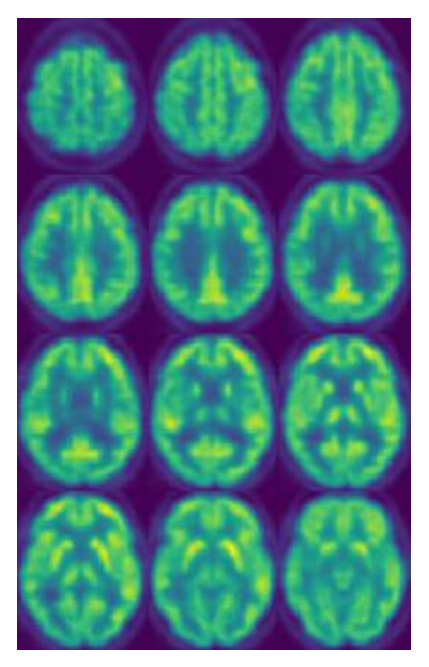
\includegraphics[width=.3\linewidth]{Graphics/ch4/originalImage.eps}}\quad
	\subfloat[\ac{FA} reconstruction]
	{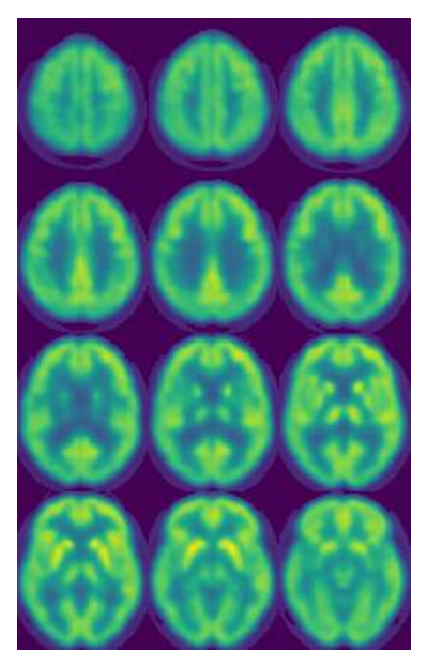
\includegraphics[width=.3\linewidth]{Graphics/ch4/transformedFA.eps}\label{fig:reconstructionFA}}\quad
	\subfloat[\ac{ICA} reconstruction]
	{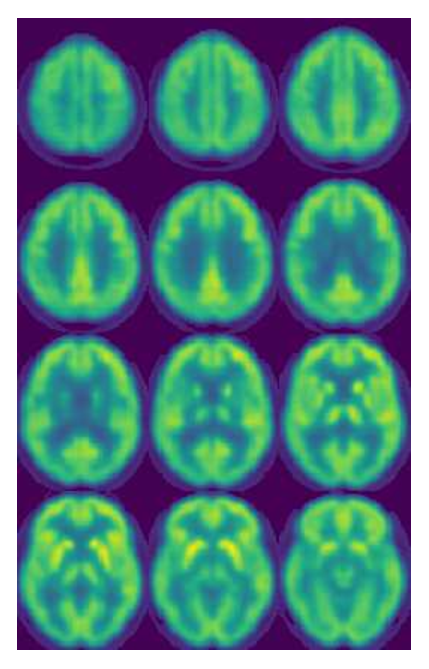
\includegraphics[width=.3\linewidth]{Graphics/ch4/transformedICA.eps}}
	\caption[Original PET image and its reconstruction using FA or ICA.]{Original PET image from the ADNI-PET dataset, and examples of reconstruction using \ac{FA} or \ac{ICA}, with 10 components.}\label{fig:comparisonReconstructions}
\end{figure}


\subsection{Factor Analysis}
\acf{FA} was used in \cite{Martinez201141,Martinez-Murcia20129676} to perform feature extraction in \ac{CAD} systems. This strategy assumes that each image in the database is a realization of a given experiment. \ac{FA} then models each of the $N$ observations (or subjects) as the expression of $c$ unobserved variables, known as factors. The model follows the general decomposition equation (Eq. \ref{eq:generalDecomposition}), but assuming that the dataset matrix $\mathbf{X}$ is zero-centred. That is, that we have subtracted the mean prior to the computation. In matrix form, Eq. \ref{eq:generalDecomposition} can be rewritten as:

\begin{equation}\label{eq:factoranalysis}
\mathbf{X} -\boldsymbol{\mu}= \mathbf{S}\mathbf{W} +  \boldsymbol{\epsilon}
\end{equation}

The columns of $\mathbf{W}$ are known as factors, and the rows of $\mathbf{S}$ are known as loadings  (similar to the concept of component loading and component scores in \ac{PCA}). Thanks to this, we can convert the original dataset $\mathbf{X}$ of size $N\times f$ into $\mathbf{S}$, of size $N\times c$. The procedure of computing the decomposition imposes some assumptions on $\mathbf{W}$: 
\begin{itemize}
	\item $\mathbf{W}$ and $\boldsymbol{\epsilon}$ must be independent. 
	\item $E[\mathbf{W}] = 0$. 
	\item $\text{Cov}(\mathbf{W}) = \mathbf{I}$, which ensures that the factors are uncorrelated. 
\end{itemize}

Now we can rewrite Eq.~\ref{eq:factoranalysis} as:
\begin{equation}\label{eq:fastep1}
	\text{Cov}(\mathbf{X} -\boldsymbol{\mu})= \text{Cov}(\mathbf{S}\mathbf{W} +  \boldsymbol{\epsilon})
\end{equation} 

Under the previous constraints, and setting $\boldsymbol{\Sigma} = \text{Cov}(\mathbf{X} -\boldsymbol{\mu})$, Eq.~\ref{eq:fastep1} becomes:
\begin{equation}
	\boldsymbol{\Sigma} = \mathbf{S}\text{Cov}(\mathbf{W})\mathbf{S}^T - \text{Cov}(\boldsymbol{\epsilon})
\end{equation}

Since $\text{Cov}(\mathbf{W}) = \mathbf{I}$, and making $\text{Cov}(\boldsymbol{\epsilon})=\boldsymbol{\Psi}$, the diagonal matrix containing the specific variances of the reconstruction error, we obtain the alternative form of \ac{FA}: 
\begin{equation}
\boldsymbol{\Sigma} = \mathbf{S}\mathbf{S}^T - \boldsymbol{\Psi}
\end{equation}

The mean $\boldsymbol{\mu}$, and the matrices $\mathbf{S}$ and $\boldsymbol{\Psi}$ are obtained via Maximum Likelihood estimation. To guarantee an unique solution, we impose that $\mathbf{S}^T\boldsymbol{\Psi}^{-1}\mathbf{S}$ is a diagonal matrix. Then, we obtain the parameters by maximizing the log-likelihood given by the following expression: 
\begin{equation}
	\ell(\mu,\mathbf{S},\boldsymbol{\Psi}) = - \frac{np}{2}\log{2\pi}- \frac{n}{2}\log{\left|\mathbf{SS}^T + \boldsymbol{\Psi}\right|} - \frac{1}{2}\sum_{i=1}^{n}(\mathbf{x}_i-\mu)^T(\mathbf{SS}^T+\boldsymbol{\Psi})(\mathbf{x}_i-\mu)
\end{equation} 

\ac{FA} differs from \ac{PCA} mainly because it performs an estimation of the noise, and needs the number of factors $c$ as an input. Choosing $c$ is not a naive task. A large $c$ can yield a small reconstruction error, but the factors will not be representative enough, leading to overfitting of the subsequent model. Conversely, a small $c$ can lead to a large reconstruction error, causing information loss. We have computed the reconstruction error variance over the ADNI-PET dataset, and plotted it in Figure~\ref{fig:error} (similar graphs can be obtained for other databases. This proves that the error is assymptotical as we increase $c$, and therefore, once arrived at certain error, the improvements are not significant. To observe how the error affects the reconstruction, in Figure~\ref{fig:reconstructionFA} we can compare a reconstructed image with its corresponding original. 

\begin{figure}[ht]
	\centering
	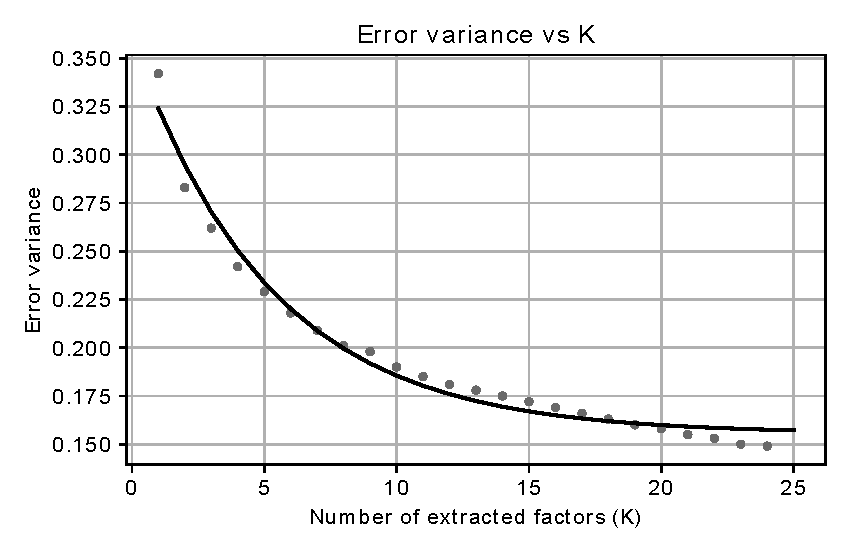
\includegraphics[width=0.5\linewidth]{Graphics/ch4/varError-K-ADNI}
	\caption[Variance of reconstruction error in \ac{FA}.]{Specific variance of reconstruction error $\Psi$ using \ac{FA}, in function of number of factors extracted ($K$) for ADNI-PET database (the behaviour is similar in other datasets).}
	\label{fig:error}
\end{figure}

\subsection{Independent Component Analysis}
\acf{ICA} \cite{Hyvarinen2000} is an algorithm that performs decomposition imposing that the resulting components must be independent. It was used in \cite{Alvarez2009,Martinez201141,Martinez-Murcia20129676} as part of a \ac{CAD} system, and it had been used in other medical imaging applications such as segmentation \cite{DeMartino2007}. 

\ac{ICA} was born as a solution to the \textit{blind source separation} problem, in which the aim is to estimate $c$ independent sources from a series of mixed signals \cite{Hyvarinen2000}. To do so, we assume the source signals to be non-gaussian, in addition to the independence assumption that we mentioned before. That is why their authors consider \ac{ICA} to be a non-gaussian version of \ac{FA} \cite{Hyvaerinen2003}, although due to this assumption, the results are very different to those obtained in \ac{FA}. 

Unlike \ac{FA}, \ac{ICA} does not account for noise in the estimation procedure, and therefore the equation remains: 
\begin{equation}\label{eq:icaecuation}
\mathbf{X} = \mathbf{W}\mathbf{S}
\end{equation}
where $\mathbf{S}$ are the component scores and $\mathbf{W}$ are the component loading, `sources' or `mixing matrix'. Given that \ac{ICA} lacks a noise term, there is a procedure called \textit{whitening} that must be applied for the algorithm to converge \cite{Hyvarinen2000}. The whitening implies a linear transformation of the $i$-th observed variable $\mathbf{x}_i$ into a \textit{white} vector $\tilde{\mathbf{x}}_i$ so that its covariance matrix equals the identity: 

\begin{equation}
E\{\tilde{\mathbf{x}}_i \tilde{\mathbf{x}}_i^T\}=\mathbf{I}
\end{equation}

This procedure is often performed using the \acf{EVD} of the covariance matrix $E\{\mathbf{x}_i \mathbf{x}_i^T\} = \mathbf{E}\mathbf{D}\mathbf{E}^T$. $\mathbf{E}$ is the covariance matrix containing the eigenvectors of $E\{\mathbf{x}_i \mathbf{x}_i^T\}$, and $\mathbf{D}$ is a diagonal matrix whose diagonal elements are the eigenvalues of $E\{\mathbf{x}_i \mathbf{x}_i^T\}$. Whitening is done using the following equation: 

\begin{equation}
\tilde{\mathbf{x}}_i= \mathbf{E}\mathbf{D}^{-1/2}\mathbf{E}^T\mathbf{x}_i
\end{equation}

This procedure transform the mixing matrix to:
\begin{equation}
\tilde{\mathbf{x}}_i = \mathbf{E}\mathbf{D}^{-1/2}\mathbf{E}^T \mathbf{W}\mathbf{s}_i
\end{equation}
which is indeed orthogonal, as can be seen here:
\begin{equation}
 E\{\tilde{\mathbf{x}}_i\tilde{\mathbf{x}}_i^T\} = \tilde{\mathbf{W}} E\{\tilde{\mathbf{s}}_i\tilde{\mathbf{s}}_i^T\}\tilde{\mathbf{W}}^T 	=\tilde{\mathbf{W}}\tilde{\mathbf{W}}^T=\mathbf{I}
\end{equation}
 
This property reduces the number of parameters to be estimated, since an orthogonal matrix contains $n(n-1)/2$ degrees of freedom, in contrast to the $n^2$ degrees of freedom of the original mixing matrix $\mathbf{W}$. 

Thanks to the central limit theorem, we assume that the sum of a large number of independent random variables tends will be approximately normally distributed, regardless of the individual statistical distributions \cite{Rice2006}. This property is used to maximize non-gaussianity and independence in the sources using any independence criteria such as the kurtosis or negentropy in any of the proposed algorithms. In this work, we will use the FastICA algorithm. 

\subsubsection{FastICA}
FastICA is a block fixed-point iteration algorithm \cite{Oja1997,FastICA99} based on negentropy as a non-gaussianity measure. Fixed-point algorithms are converge faster than adaptive algorithms \cite{FastICA99}. The FastICA algorithm can be considered a neural algorithm \cite{Hyvarinen2000}, where the weight vector $\mathbf{w}$ can be updated using a learning rule. FastICA defines a learning rule that finds a direction $\mathbf{w}$, a unit vector such that the projection $\mathbf{w}^T\mathbf{x}_i$ maximizes non-gaussianity \cite{FastICA99}. 

The non-gaussianity measure used here is the negative entropy, or negentropy. The negentropy is a form of differential entropy, which for a random vector $\mathbf{y}$ is defined as: 
\begin{equation}
	J(\mathbf{y})=H(\mathbf{y}_{gauss})-H(\mathbf{y})
\end{equation}
where  $\mathbf{y}_{gauss}$ and $\mathbf{y}$ share the same covariance matrix, although $\mathbf{y}$ is not a gaussian random variable, and $\mathbf{y}_{gauss}$ is. There are many approximations to negentropy. The FastICA defines negentropy using the function: 
\begin{equation}
J(y)\propto [E\{G(y)\}-E\{G(\nu)\}]^2
\end{equation}
where we assume that $y$ is of zero mean and unit variance, $\nu$ is a Gaussian variable sharing the same mean and variance, and $G(x)$ is any non-quadratic function. Many functions have been proposed, but in the FastICA algorithm we use either $G(x)_1 = (1/a_1) \log\cosh a_1 x$ with $1<a_1<2$ or $G(x)_2 = \exp(-x^2/2)$ \cite{FastICA99}. 

With these measures, we can compute the derivatives of these functions by: 
\begin{align}
g_1(x) & =\tanh(a_1 x), \\
g_2(x) & = x\exp(- x^2/2)
\end{align} 

The algorithm for the one-unit version of FastICA can be defined \cite{FastICA99} as:
\begin{enumerate}
	\item Choose an initial (e.g. random) weight vector ${\bf w}$.
	\item Let  ${\bf w}^+=E\{{\bf x}g({\bf w}^T{\bf x})\}-E\{g'({\bf w}^T{\bf x})\}{\bf w}$
	\item Let  ${\bf w}={\bf w}^+/\Vert{\bf w}^+\Vert$
	\item If not converged, go back to 2.
\end{enumerate}

The algorithm considers that the values of $\mathbf{w}$ converge when their dot product is close to 1, that is, they are pointing in the same direction. Note that the expectations are computed as the sample mean in the FastICA algorithm. Additional modifications were presented in \cite{Hyvarinen2000}, in which step 2 is converted to a Newton iteration and further simplification is performed. 

This is the algorithm for one computational unit, or neuron, which computes one component. However, the procedure can be extended to $c$ components by defining $c$ neurons with weight vectors ${\bf w}_1,...,{\bf w}_c$ so that $\mathbf{W} = ({\bf w}_1,...,{\bf w}_n)^T$. The outputs ${\bf w}_1^T{\bf x},...,{\bf w}_n^T{\bf x}$ must be decorrelated to prevent them from converging to the same maxima, using three methods proposed in \cite{Hyvarinen2000}. 

The method used in this work uses a two-step iterative algorithm \cite{Hyvarinen2000} to decorrelate the outputs after each iteration: 
\begin{enumerate}
\item Let $\mathbf{W} = \mathbf{W}/\sqrt{\lVert\mathbf{W}\mathbf{W}^T\rVert}$. 
\item Let $\mathbf{W} = \frac{3}{2} \mathbf{W}-\frac{1}{2} \mathbf{W} \mathbf{W}^T  \mathbf{W}$
\end{enumerate}

And repeat step 2 until convergence. For simplicity, the norm in step 1 can be computed as any norm but the Frobenius norm, for example, the L2-norm or the largest absolute row sum. 

\section{Results}
In this work we will analyse the behaviour of the system proposed in the introduction and illustrated at Figure~\ref{fig:pipelineDecomposition}. The system comprises the selection of the most relevant voxels using filtering methods (we will focus on $t$-test, relative entropy and wilcoxon) and a feature decomposition of these using either \ac{FA} or \ac{ICA}. Finally, the feature vectors are classified using a \ac{SVC} with linear kernel, and performance values are obtained via cross-validation (see Section~\ref{sec:validation} for more information). 

We vary the number of selected voxels and the number of factors or components depending on the algorithm and the dataset used and evaluate the system with those characteristics. That way, we obtain an estimation of the performance of the system in different situations, so that we can draw conclusions on the disease patterns and the ability of the system in the detection of different diseases. 

\subsection{Alzheimer's Disease}
We begin by applying the proposed feature selection plus decomposition pipeline to the two functional neuroimaging datasets: ADNI-PET and VDLN-HMPAO. For this experiment we will use a maximum of $20,000$ selected voxels and $25$ components. 

\subsubsection{Factor Analysis}\label{sec:results_FA_AD}
First, we use \ac{FA} as a decomposition technique. In Figure~\ref{fig:accuracyMeanFA-AD} we average the accuracy over the number of voxels or the number of components respectively, to look at how these variables affect the performance of the system, and we do this for the three filtering methods used. 

\begin{figure}	\centering
	\subfloat[]{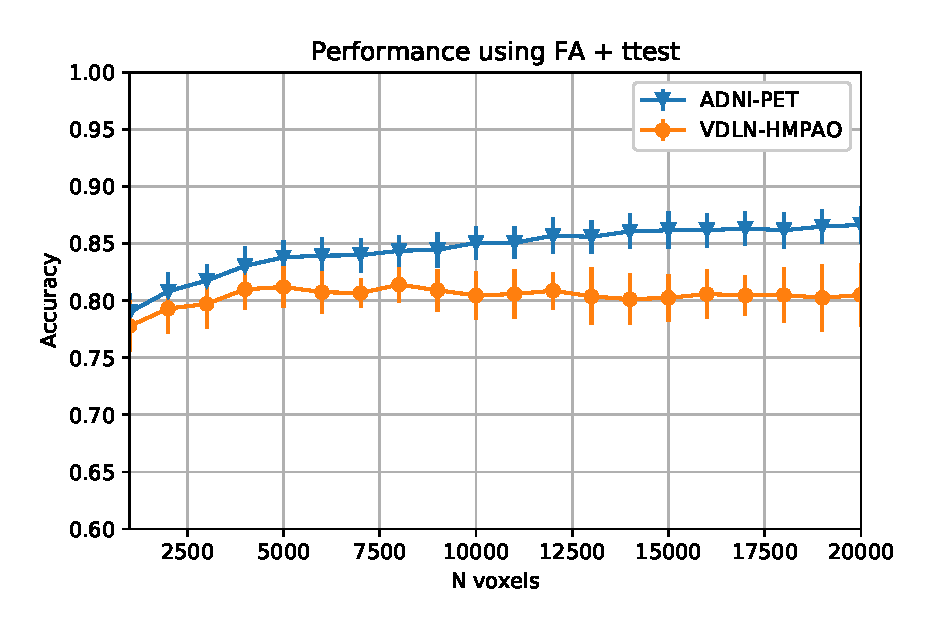
\includegraphics[width=0.49\linewidth]{Graphics/ch4/accuracyMeanSTD-FA_vsN_ttest_AD.eps}\label{fig:AD-AV-FA-TTEST-VSN}}
	\subfloat[]{\includegraphics[width=0.49\linewidth]{Graphics/ch4/accuracyMeanSTD-FA_vsK_ttest_AD.eps}\label{fig:AD-AV-FA-TTEST-VSK}}
	
	\subfloat[]{\includegraphics[width=0.49\linewidth]{Graphics/ch4/accuracyMeanSTD-FA_vsN_entropy_AD.eps}\label{fig:AD-AV-FA-ENTROPY-VSN}}
	\subfloat[]{\includegraphics[width=0.49\linewidth]{Graphics/ch4/accuracyMeanSTD-FA_vsK_entropy_AD.eps}\label{fig:AD-AV-FA-ENTROPY-VSK}}
	
	\subfloat[]{\includegraphics[width=0.49\linewidth]{Graphics/ch4/accuracyMeanSTD-FA_vsN_wilcoxon_AD.eps}\label{fig:AD-AV-FA-WILCOXON-VSN}}
	\subfloat[]{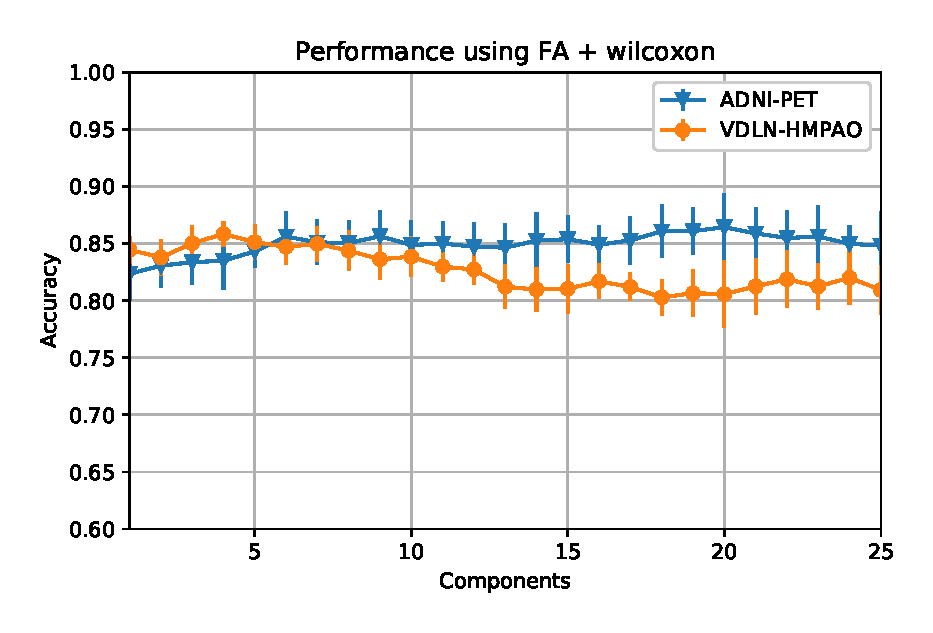
\includegraphics[width=0.49\linewidth]{Graphics/ch4/accuracyMeanSTD-FA_vsK_wilcoxon_AD.eps}\label{fig:AD-AV-FA-WILCOXON-VSK}}
	
	\caption{Average performance and standard deviation of the proposed system using the two \ac{AD} datasets, \ac{FA} and the three feature selection criteria: $t$-test (\protect\subref{fig:AD-AV-FA-TTEST-VSN} and \protect\subref{fig:AD-AV-FA-TTEST-VSK}), relative entropy (\protect\subref{fig:PKS-AV-FA-ENTROPY-VSN} and \protect\subref{fig:AD-AV-FA-ENTROPY-VSK}) and wilcoxon (\protect\subref{fig:AD-AV-FA-WILCOXON-VSN} and \protect\subref{fig:AD-AV-FA-WILCOXON-VSK}). } 
	\label{fig:accuracyMeanFA-AD}
\end{figure}

We can observe that the results are always better when using the ADNI-PET dataset than with the VDLN-HMPAO, and this is especially notorious when using the relative entropy selection criterion. The performance tends to slightly increase with the number of voxels selected, but it is not the case with the number of components. By looking at figures \ref{fig:AD-AV-FA-TTEST-VSK}, \ref{fig:AD-AV-FA-ENTROPY-VSK} and \ref{fig:AD-AV-FA-WILCOXON-VSK}, it seems that a relatively small number of components (approximately 6) is enough to obtain good performance, and afterwards, the performance holds or even decreases. 

\subsubsection{Independent Component Analysis}
In this section, we compute the results of applying \ac{ICA} to the ADNI-PET and VDLN-HMPAO datasets. Figure~\ref{fig:accuracyMeanICA-AD} depicts the average accuracy over the number of voxels or the number of components respectively for the different selection criteria. 

\begin{figure}
	\centering
	\subfloat[]{\includegraphics[width=0.49\linewidth]{Graphics/ch4/accuracyMeanSTD-ICA_vsN_ttest_AD.eps}\label{fig:AD-AV-ICA-TTEST-VSN}}
	\subfloat[]{\includegraphics[width=0.49\linewidth]{Graphics/ch4/accuracyMeanSTD-ICA_vsK_ttest_AD.eps}\label{fig:AD-AV-ICA-TTEST-VSK}}
	
	\subfloat[]{\includegraphics[width=0.49\linewidth]{Graphics/ch4/accuracyMeanSTD-ICA_vsN_entropy_AD.eps}\label{fig:AD-AV-ICA-ENTROPY-VSN}}
	\subfloat[]{\includegraphics[width=0.49\linewidth]{Graphics/ch4/accuracyMeanSTD-ICA_vsK_entropy_AD.eps}\label{fig:AD-AV-ICA-ENTROPY-VSK}}
	
	\subfloat[]{\includegraphics[width=0.49\linewidth]{Graphics/ch4/accuracyMeanSTD-ICA_vsN_wilcoxon_AD.eps}\label{fig:AD-AV-ICA-WILCOXON-VSN}}
	\subfloat[]{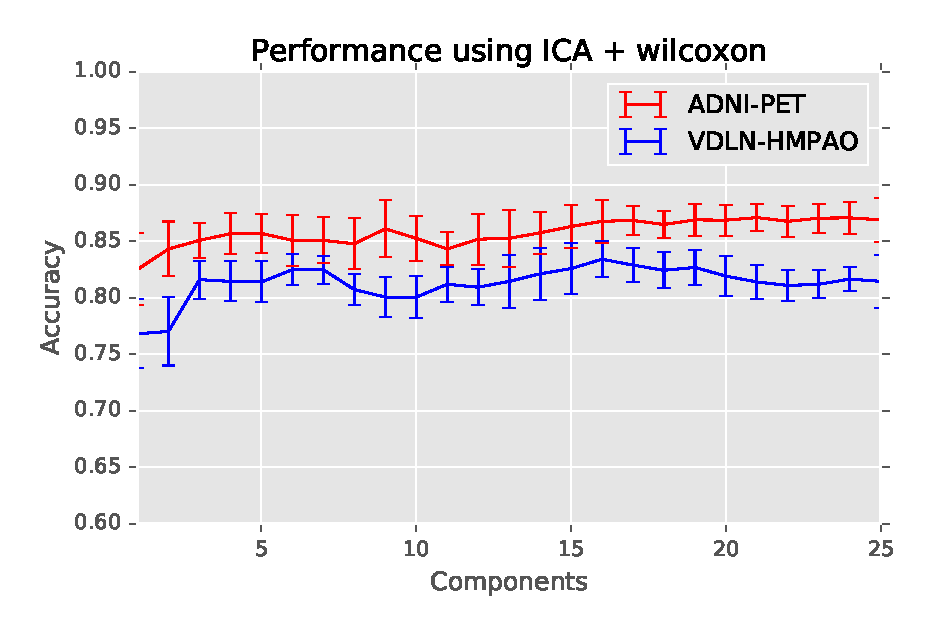
\includegraphics[width=0.49\linewidth]{Graphics/ch4/accuracyMeanSTD-ICA_vsK_wilcoxon_AD.eps}\label{fig:AD-AV-ICA-WILCOXON-VSK}}
	
	\caption{Average performance and standard deviation of the proposed system using the three \ac{AD} datasets, \ac{ICA} and the three feature selection criteria: $t$-test (\protect\subref{fig:AD-AV-ICA-TTEST-VSN} and \protect\subref{fig:AD-AV-ICA-TTEST-VSK}), relative entropy (\protect\subref{fig:AD-AV-ICA-ENTROPY-VSN} and \protect\subref{fig:AD-AV-ICA-ENTROPY-VSK}) and wilcoxon (\protect\subref{fig:AD-AV-ICA-WILCOXON-VSN} and \protect\subref{fig:AD-AV-ICA-WILCOXON-VSK}). } 
	\label{fig:accuracyMeanICA-AD}
\end{figure}

The case is similar to the one presented in Section~\ref{sec:results_FA_AD}, where the performance slightly improves when increasing the number of selected voxels. The performance is again better when using the ADNI-PET dataset than with the VDLN-HMPAO, although the behaviour is similar. 

The results change when varying the number of components. In this case, although good performance is obtained within the first 5 components in most cases, the performance does not decrease with a higher number, and sometimes increases (for example, in the case of \ac{ICA} and the $t$-test or the wilcoxon selection criteria). 
\subsubsection{At the Operation Point}
Now we focus on non-averaged values, the values for which our system is optimal: the operation point. In this scenario we see that the tendency is that all systems behave similarly. The accuracy vary slightly with the number of components selected to build the model almost in any case, and there is a steep increase in the performance within the first five components.

\begin{figure}
	\centering
	\subfloat[]{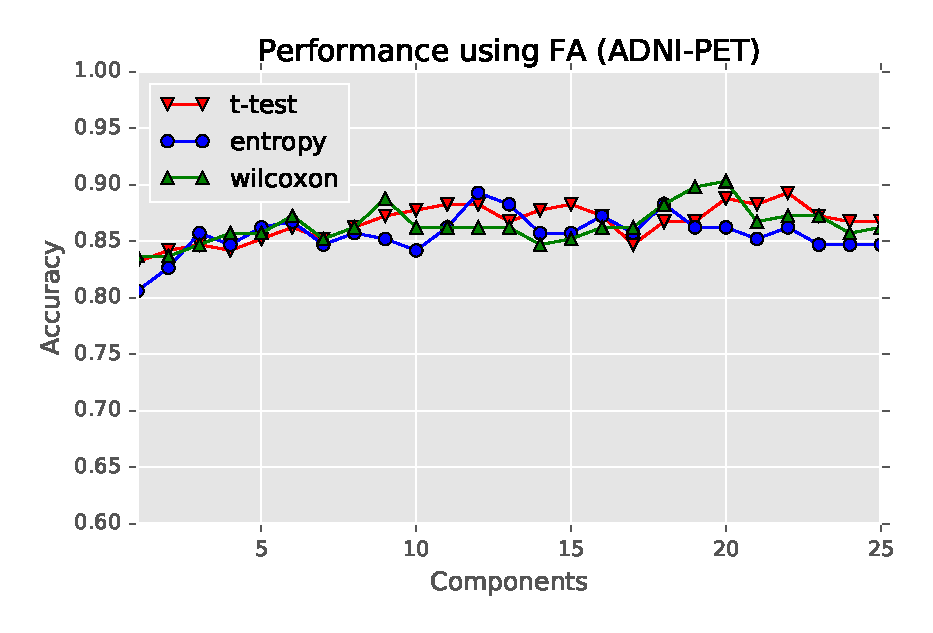
\includegraphics[width=0.49\linewidth]{Graphics/ch4/accuracyOP-FA_vsN_comparison_ADNI-PET.eps}\label{fig:ADNI-PET-FA-OP-VSK}}
	\subfloat[]{\includegraphics[width=0.49\linewidth]{Graphics/ch4/accuracyOP-ICA_vsN_comparison_ADNI-PET.eps}\label{fig:ADNI-PET-ICA-OP-VSK}}
	
	\subfloat[]{\includegraphics[width=0.49\linewidth]{Graphics/ch4/accuracyOP-FA_vsN_comparison_VDLN-HMPAO.eps}\label{fig:VDLN-HMPAO-FA-OP-VSK}}
	\subfloat[]{\includegraphics[width=0.49\linewidth]{Graphics/ch4/accuracyOP-ICA_vsN_comparison_VDLN-HMPAO.eps}\label{fig:VDLN-HMPAO-ICA-OP-VSK}}
	
	\caption{Performance of the proposed system using the two \ac{AD} datasets: ADNI-PET and VDLN-HMPAO at the operation point, and how they vary over the number of components used in the decomposition. } 
	\label{fig:accuracyOP-AD}
\end{figure}

A particular case is the combination of \ac{FA} and the relative entropy selection criteria applied to the VDLN-HMPAO dataset. In this case there seems to be a trend to achieve a maximum performance at between 8-10 components. But it is an individual behaviour that does not reproduce on the other datasets or strategies, therefore it must be related to the dataset itself. 
% HASTA AQUI

As for the variation of the performance when increasing the number of selected voxels, we can see that there is always a tendency of slightly increase in both datasets and decomposition strategies, as can be seen in Figure~\ref{fig:accuracyOP-ADvsN}. There, the best performance

\begin{figure}
	\centering
	\subfloat[]{\includegraphics[width=0.49\linewidth]{Graphics/ch4/accuracyOP-FA_vsK_comparison_ADNI-PET.eps}\label{fig:ADNI-PET-FA-OP-VSN}}
	\subfloat[]{\includegraphics[width=0.49\linewidth]{Graphics/ch4/accuracyOP-ICA_vsK_comparison_ADNI-PET.eps}\label{fig:ADNI-PET-ICA-OP-VSN}}
	
	\subfloat[]{\includegraphics[width=0.49\linewidth]{Graphics/ch4/accuracyOP-FA_vsK_comparison_VDLN-HMPAO.eps}\label{fig:VDLN-HMPAO-FA-OP-VSN}}
	\subfloat[]{\includegraphics[width=0.49\linewidth]{Graphics/ch4/accuracyOP-ICA_vsK_comparison_VDLN-HMPAO.eps}\label{fig:VDLN-HMPAO-ICA-OP-VSN}}
	
	\caption{Performance of the proposed system using the two \ac{AD} datasets: ADNI-PET and VDLN-HMPAO at the operation point, and how they vary over the number of selected voxels. } 
	\label{fig:accuracyOP-ADvsN}
\end{figure}

In Table~\ref{tab:featureAD} we show the performance values obtained at the operation point for our different test combining decomposition algorithms and selection criteria, for the two datasets analysed in this section. It is 

\begin{table}
	\myfloatalign
	\begin{tabularx}{\linewidth}{Xllccc}
		\tableheadline{DB} & \tableheadline{Dec.} & \tableheadline{Criterion} & \tableheadline{Accuracy} & \tableheadline{Sensitivity} & \tableheadline{Specificity}\\
		\toprule
		\multirow{6}{1.7cm}{ADNI- PET} & \multirow{3}{*}{\ac{FA}} & t-test & $ 0.893 \pm 0.074 $ & $ 0.886 \pm 0.119 $ & $ 0.901 \pm 0.101 $ \\
		&  & entropy & $ 0.893 \pm 0.074 $ & $ 0.894 \pm 0.092 $ & $ 0.891 \pm 0.088 $ \\
		&  & wilcoxon & $ 0.903 \pm 0.066 $ & $ 0.917 \pm 0.079 $ & $ 0.891 \pm 0.082 $ \\
		\cline{2-6}
		& \multirow{3}{*}{\ac{ICA}} & t-test & $ 0.903 \pm 0.071 $ & $ 0.893 \pm 0.100 $ & $ 0.910 \pm 0.107 $ \\
		&  & entropy & $ 0.898 \pm 0.059 $ & $ 0.917 \pm 0.088 $ & $ 0.881 \pm 0.084 $ \\
		&  & wilcoxon & $ 0.903 \pm 0.066 $ & $ 0.906 \pm 0.097 $ & $ 0.901 \pm 0.094 $ \\ \midrule
		\multirow{6}{*}{\parbox{1.5cm}{VDLN-HMPAO}} & \multirow{3}{*}{\ac{FA}} & t-test & $ 0.885 \pm 0.076 $ & $ 0.890 \pm 0.127 $ & $ 0.875 \pm 0.149 $ \\
		&  & entropy & $ 0.896 \pm 0.092 $ & $ 0.907 \pm 0.150 $ & $ 0.875 \pm 0.139 $ \\
		&  & wilcoxon & $ 0.885 \pm 0.076 $ & $ 0.923 \pm 0.130 $ & $ 0.825 \pm 0.154 $ \\
		\cline{2-6}
		& \multirow{3}{*}{\ac{ICA}} & t-test & $ 0.885 \pm 0.073 $ & $ 0.923 \pm 0.130 $ & $ 0.825 \pm 0.154 $ \\
		&  & entropy & $ 0.885 \pm 0.076 $ & $ 0.903 \pm 0.132 $ & $ 0.850 \pm 0.130 $ \\
		&  & wilcoxon & $ 0.885 \pm 0.076 $ & $ 0.907 \pm 0.130 $ & $ 0.850 \pm 0.152 $ \\
		\bottomrule
	\end{tabularx}
	\caption[Performance values for the Alzheimer's datasets]{Accuracy, sensitivity, specificity, and their standard deviation at the operation point for each method and its corresponding feature selection criterion, using two \protect\ac{AD} datasets. }
	\label{tab:featureAD}
\end{table}




\FloatBarrier

% DESDE AQUI
\subsection{Parkinson's Disease}
Now we will look at how the proposed \ac{CAD} system behaves when applied to the three DaTSCAN datasets: VDLN-DAT, VDLV-DAT and PPMI-DAT. For this experiment we will use a maximum of $1500$ selected voxels and $25$ components. 

\subsubsection{Factor Analysis}
Firstly, we will explore the average behaviour of the system that uses \ac{FA} as a decomposition technique. For this purpose, as in previous sections, Figure~\ref{fig:accuracyMeanFA-PKS} shows how the average performance varies when varying the number of voxels selected and the number of components extracted. 

\begin{figure}
	\centering
	\subfloat[]{\includegraphics[width=0.49\linewidth]{Graphics/ch4/accuracyMeanSTD-FA_vsN_ttest_PKS.eps}\label{fig:PKS-AV-FA-TTEST-VSN}}
	\subfloat[]{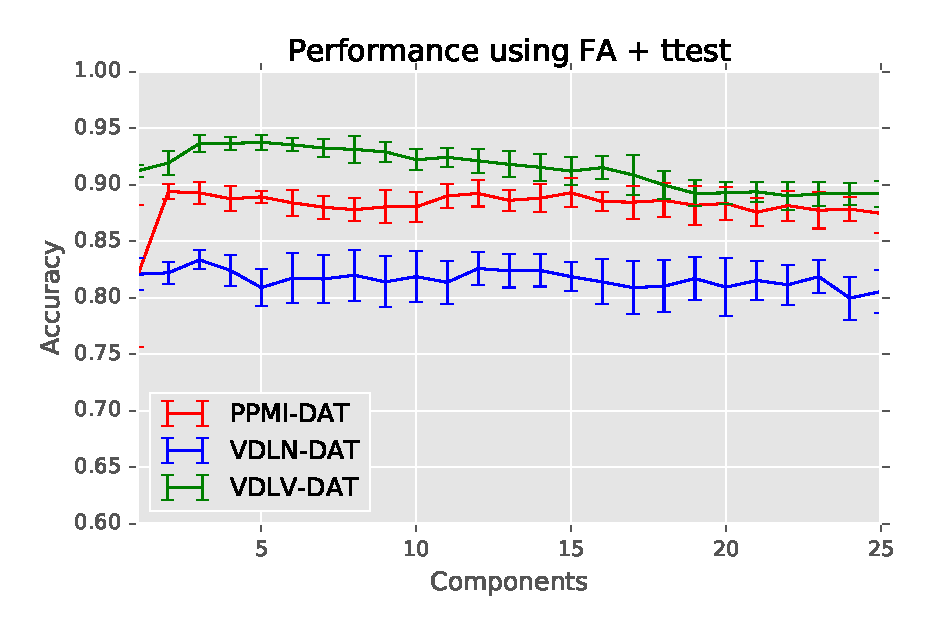
\includegraphics[width=0.49\linewidth]{Graphics/ch4/accuracyMeanSTD-FA_vsK_ttest_PKS.eps}\label{fig:PKS-AV-FA-TTEST-VSK}}
	
	\subfloat[]{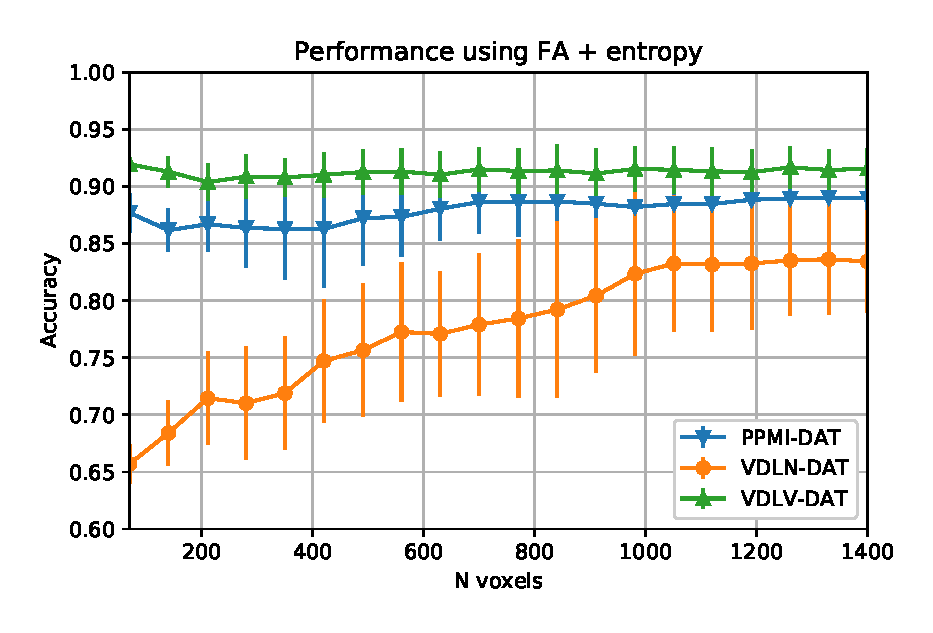
\includegraphics[width=0.49\linewidth]{Graphics/ch4/accuracyMeanSTD-FA_vsN_entropy_PKS.eps}\label{fig:PKS-AV-FA-ENTROPY-VSN}}
	\subfloat[]{\includegraphics[width=0.49\linewidth]{Graphics/ch4/accuracyMeanSTD-FA_vsK_entropy_PKS.eps}\label{fig:PKS-AV-FA-ENTROPY-VSK}}
	
	\subfloat[]{\includegraphics[width=0.49\linewidth]{Graphics/ch4/accuracyMeanSTD-FA_vsN_wilcoxon_PKS.eps}\label{fig:PKS-AV-FA-WILCOXON-VSN}}
	\subfloat[]{\includegraphics[width=0.49\linewidth]{Graphics/ch4/accuracyMeanSTD-FA_vsK_wilcoxon_PKS.eps}\label{fig:PKS-AV-FA-WILCOXON-VSK}}
	
	\caption{Average performance and standard deviation of the proposed system using the three \ac{PKS} datasets, \ac{FA} and the three feature selection criteria: $t$-test (\protect\subref{fig:PKS-AV-FA-TTEST-VSN} and \protect\subref{fig:PKS-AV-FA-TTEST-VSK}), relative entropy (\protect\subref{fig:PKS-AV-FA-ENTROPY-VSN} and \protect\subref{fig:PKS-AV-FA-ENTROPY-VSK}) and wilcoxon (\protect\subref{fig:PKS-AV-FA-WILCOXON-VSN} and \protect\subref{fig:PKS-AV-FA-WILCOXON-VSK}). } 
	\label{fig:accuracyMeanFA-PKS}
\end{figure}

In this case there is a clear difference between datasets, since some of them are more complex than others, usually due to a typical acquisition procedure in DaTSCAN. In the VDLN-DAT, the images were often composed only of a few cuts around the striatum, whereas in PPMI and VDLV-DAT this rarely happens. That would explain the average outperformance of these two datasets over the VDLN-DAT in almost all cases. 

Their behaviours are consistent. Usually, there is no variation with the number of voxel selected (except in the obvious case of the VDLN-DAT dataset and the relative entropy selection criterion). However, there are repeated trends regarding the number of components or factors used in the computation. We can see that the performance increases in the first components, and once we have achieve a decent number (between 4 and 6), the performance starts to decrease. This could mean that the decomposition in more than 5 or 6 components only introduces noise and leads to a wrong decomposition. 

Again, this behaviour is consistent with the VDLN-DAT dataset, except for one case. It does seem that the interaction between the VDLN-DAT dataset and the relative entropy selection criterion leads to a wrong model. We will explore this question later, in the discussion. 

\subsubsection{Independent Component Analysis}
\begin{figure}
	\subfloat[]{\includegraphics[width=0.49\linewidth]{Graphics/ch4/accuracyMeanSTD-ICA_vsN_ttest_PKS.eps}\label{fig:PKS-AV-ICA-TTEST-VSN}}
	\subfloat[]{\includegraphics[width=0.49\linewidth]{Graphics/ch4/accuracyMeanSTD-ICA_vsK_ttest_PKS.eps}\label{fig:PKS-AV-ICA-TTEST-VSK}}
	
	\subfloat[]{\includegraphics[width=0.49\linewidth]{Graphics/ch4/accuracyMeanSTD-ICA_vsN_entropy_PKS.eps}\label{fig:PKS-AV-ICA-ENTROPY-VSN}}
	\subfloat[]{\includegraphics[width=0.49\linewidth]{Graphics/ch4/accuracyMeanSTD-ICA_vsK_entropy_PKS.eps}\label{fig:PKS-AV-ICA-ENTROPY-VSK}}
	
	\subfloat[]{\includegraphics[width=0.49\linewidth]{Graphics/ch4/accuracyMeanSTD-ICA_vsN_wilcoxon_PKS.eps}\label{fig:PKS-AV-ICA-WILCOXON-VSN}}
	\subfloat[]{\includegraphics[width=0.49\linewidth]{Graphics/ch4/accuracyMeanSTD-ICA_vsK_wilcoxon_PKS.eps}\label{fig:PKS-AV-ICA-WILCOXON-VSK}}
	
	\caption{Average performance and standard deviation of the proposed system using the three \ac{PKS} datasets, \ac{ICA} and the three feature selection criteria: $t$-test (\protect\subref{fig:PKS-AV-ICA-TTEST-VSN} and \protect\subref{fig:PKS-AV-ICA-TTEST-VSK}), relative entropy (\protect\subref{fig:PKS-AV-ICA-ENTROPY-VSN} and \protect\subref{fig:PKS-AV-ICA-ENTROPY-VSK}) and wilcoxon (\protect\subref{fig:PKS-AV-ICA-WILCOXON-VSN} and \protect\subref{fig:PKS-AV-ICA-WILCOXON-VSK}). } 
	\label{fig:accuracyMeanICA-PKS}
\end{figure}


\subsubsection{At the Operation Point}

\begin{figure}
	\subfloat[]{\includegraphics[width=0.49\linewidth]{Graphics/ch4/accuracyOP-FA_vsN_comparison_PPMI-DAT.eps}\label{fig:PPMI-DAT-FA-OP}}
	\subfloat[]{\includegraphics[width=0.49\linewidth]{Graphics/ch4/accuracyOP-ICA_vsN_comparison_PPMI-DAT.eps}\label{fig:PPMI-DAT-ICA-OP}}
	
	\subfloat[]{\includegraphics[width=0.49\linewidth]{Graphics/ch4/accuracyOP-FA_vsN_comparison_VDLN-DAT.eps}\label{fig:VDLN-DAT-FA-OP}}
	\subfloat[]{\includegraphics[width=0.49\linewidth]{Graphics/ch4/accuracyOP-ICA_vsN_comparison_VDLN-DAT.eps}\label{fig:VDLN-DAT-ICA-OP}}
	
	\subfloat[]{\includegraphics[width=0.49\linewidth]{Graphics/ch4/accuracyOP-FA_vsN_comparison_VDLV-DAT.eps}\label{fig:VDLV-DAT-FA-OP}}
	\subfloat[]{\includegraphics[width=0.49\linewidth]{Graphics/ch4/accuracyOP-ICA_vsN_comparison_VDLV-DAT.eps}\label{fig:VDLV-DAT-ICA-OP}}
	
	\caption{Performance of the proposed system using the two \ac{PKS} datasets: PPMI-DAT, VDLN-DAT and VDLV-DAT at the operation point, and how they vary over the number of components used in the decomposition. } 
	\label{fig:accuracyOP-PKS}
\end{figure}


\begin{table}
	\begin{tabularx}{\linewidth}{Xllccc}
		\tableheadline{DB} & \tableheadline{Dec.} & \tableheadline{Criterion} & \tableheadline{Accuracy} & \tableheadline{Sensitivity} & \tableheadline{Specificity}\\
		\toprule
		\multirow{6}{1.7cm}{VDLN-DAT} & \multirow{3}{*}{\ac{FA}} & t-test & $ 0.856 \pm 0.111 $ & $ 0.887 \pm 0.178 $ & $ 0.795 \pm 0.164 $ \\
		&  & entropy & $ 0.890 \pm 0.098 $ & $ 0.875 \pm 0.118 $ & $ 0.910 \pm 0.116 $ \\
		&  & wilcoxon & $ 0.864 \pm 0.070 $ & $ 0.916 \pm 0.114 $ & $ 0.780 \pm 0.183 $ \\
		\cline{2-6}
		& \multirow{3}{*}{\ac{ICA}} & t-test & $ 0.864 \pm 0.101 $ & $ 0.873 \pm 0.174 $ & $ 0.840 \pm 0.166 $ \\
		&  & entropy & $ 0.907 \pm 0.075 $ & $ 0.889 \pm 0.124 $ & $ 0.935 \pm 0.131 $ \\
		&  & wilcoxon & $ 0.873 \pm 0.108 $ & $ 0.859 \pm 0.181 $ & $ 0.890 \pm 0.151 $ \\
		\midrule
		\multirow{6}{1.7cm}{VDLV-DAT} & \multirow{3}{*}{\ac{FA}} & t-test & $ 0.957 \pm 0.033 $ & $ 0.940 \pm 0.066 $ & $ 0.973 \pm 0.065 $ \\
		&  & entropy & $ 0.952 \pm 0.037 $ & $ 0.940 \pm 0.066 $ & $ 0.964 \pm 0.064 $ \\
		&  & wilcoxon & $ 0.957 \pm 0.033 $ & $ 0.940 \pm 0.066 $ & $ 0.973 \pm 0.065 $ \\
		\cline{2-6}
		& \multirow{3}{*}{\ac{ICA}} & t-test & $ 0.952 \pm 0.037 $ & $ 0.940 \pm 0.066 $ & $ 0.964 \pm 0.064 $ \\
		&  & entropy & $ 0.947 \pm 0.045 $ & $ 0.940 \pm 0.066 $ & $ 0.955 \pm 0.076 $ \\
		&  & wilcoxon & $ 0.952 \pm 0.037 $ & $ 0.940 \pm 0.066 $ & $ 0.964 \pm 0.064 $ \\
		\midrule
		\multirow{6}{1.7cm}{PPMI-DAT} & \multirow{3}{*}{\ac{FA}} & t-test & $ 0.917 \pm 0.037 $ & $ 0.918 \pm 0.095 $ & $ 0.918 \pm 0.091 $ \\
		&  & entropy & $ 0.917 \pm 0.060 $ & $ 0.918 \pm 0.076 $ & $ 0.921 \pm 0.120 $ \\
		&  & wilcoxon & $ 0.912 \pm 0.056 $ & $ 0.927 \pm 0.098 $ & $ 0.889 \pm 0.102 $ \\
		\cline{2-6}
		& \multirow{3}{*}{\ac{ICA}} & t-test & $ 0.917 \pm 0.056 $ & $ 0.900 \pm 0.095 $ & $ 0.948 \pm 0.109 $ \\
		&  & entropy & $ 0.928 \pm 0.055 $ & $ 0.909 \pm 0.091 $ & $ 0.961 \pm 0.090 $ \\
		&  & wilcoxon & $ 0.912 \pm 0.070 $ & $ 0.909 \pm 0.100 $ & $ 0.920 \pm 0.118 $ \\
		\bottomrule
		\end{tabularx}
		\caption[Performance values for the Parkinson's datasets]{Accuracy, sensitivity, specificity, and their standard deviation at the operation point for each method and its corresponding feature selection criterion, using three \protect\ac{PKS} datasets }
		\label{tab:featurePKS}
\end{table}

\section{Discussion}

Explore this: Again, this behaviour is consistent with the VDLN-DAT dataset, except for one case. It does seem that the interaction between the VDLN-DAT dataset and the relative entropy selection criterion leads to a wrong model. We will explore this question later, in the discussion. 
%************************************************
\chapter{Texture Features}\label{ch:texture}
%************************************************
\section{Introduction}
Texture analysis is any procedure intended to classify and quantify the spatial variation of voxel intensity throughout the image. In neuroimaging, they are more commonly used to classify images or to segment them (which can be also considered a form of classification). Depending on the number of variables studies, we can divide the methodology into first, second and higher order statistical texture analysis. In first-order statistics, only voxel intensity values are considered, and values such as average, variance, kurtosis or frequency (histogram) of intensity values are computed. 

Second-order statistical texture analysis is by far the most popular form. It is based on the probability of finding a pair of grey-level at a certain distance and orientation on a certain image. Most algorithms are based in the Grey Level Co-occurrence Matrix (GLCM), in which is known as Haralick Texture Analysis [59]. The GLCM can be thought of as a representation of the frequency of the adjacent pixel variations in a certain spatial direction and distance. For a three dimensional  brain image  and two different grey levels  and , at a given offset  the co-occurrence value is defined as:

\cite{Martinez-Murcia2013266,Martinez-Murcia2014}
\section{Haralick Texture Features}
\subsubsection{Gray Level Co-occurrence Matrix}
%Que son las matriz de coocurrencia y las texture features
A co-occurrence matrix is a square matrix that counts the number of repetitions of co-occurring values over an image, given an offset that measures the distance from the central to the neighbor voxels. In this work we use a modification of the widely used co-occurrence matrix defined in \cite{Philips2008}, that generalizes this matrix to a three-dimensional space. For two different gray levels $i$ and $j$, the co-occurrence matrix $\mathbf{C}$ is defined over a $n \times m \times k$ three-dimensional image $\mathbf{I}$, given an offset $\Delta$ as follows: 
\begin{equation}\label{eq:cooc3D}
\mathbf{C}_{\Delta}(i,j)=\sum_{p=(1,1,1)}^{(n,m,k)}\begin{cases} 1, & \mbox{if }\mathbf{I}(\mathbf{p})=i\mbox{ and }\mathbf{I}(\mathbf{p}+\Delta)=j \\ 0, & \mbox{otherwise}\end{cases}
\end{equation}
where $i$ and $j$ are different gray levels, $\mathbf{p}=(x,y,z)$ is the spatial position where $x=1...n, y=1...m, z=1...k$ and $\Delta=(d,d,d)$ is the offset vector, which  has been set as dependent only on the distance $d$. In this work, the 3D-GLC matrix is computed over a selected subimage, computed as defined in Sec. \ref{sec:volume}, and we have performed a rescaling of the original data into $16$ gray levels, leading to a best-performance.


\subsubsection{Haralick Texture Features}
%Parámetros de haralick. 
After computing the 3D-GLC matrix, twelve Haralick Texture Features \cite{Haralick73} are derived, using the following expressions:

\begin{center}
	\begin{tabular}{r|c}
		Energy & $\sum\limits_{i,j} \{ \mathbf{C}_{\Delta}(i,j)\}^2 $\\
		Entropy & $-\sum\limits_{i,j} \mathbf{C}_{\Delta}(i,j)*\log(\mathbf{C}_{\Delta}(i,j)) $\\
		Correlation & $\sum\limits_{i,j} {{(i-\mu_i)(j-\mu_j)\mathbf{C}_{\Delta}(i,j)}\over{\sigma_i\sigma_j}}$\\
		Contrast & $\sum\limits_{i,j} |i-j|^2 \mathbf{C}_{\Delta}(i,j)$ \\
		Variance & $\sum\limits_{i,j} (i-\mu_i)^2 \mathbf{C}_{\Delta}(i,j)+ (j-\mu_j)^2\mathbf{C}_{\Delta}(i,j)$\\
		Sum Mean & ${1 \over 2} \sum\limits_{i,j}(i\mathbf{C}_{\Delta}(i,j)+j\mathbf{C}_{\Delta}(i,j))$\\
		Inertia & $\sum\limits_{i,j}(i-j)^2*\mathbf{C}_{\Delta}(i,j)$\\
		Cluster Shade & $\sum\limits_{i,j}(i+j-\mu_x-\mu_y)^3 * \mathbf{C}_{\Delta}(i,j)$\\
		Cluster Tendency & $\sum\limits_{i,j}\{ i+j-\mu_x-\mu_y\}^4*\mathbf{C}_{\Delta}(i,j)$\\
		Homogeneity & $\sum\limits_{i,j} {\mathbf{C}_{\Delta}(i,j) \over 1+|i-j|}$\\
		Max Probability & $\max (\mathbf{C}_{\Delta})$\\
		Inverse Variance & $\sum\limits_{i,j} {\mathbf{C}_{\Delta}(i,j) \over (i-j)^2}$\\
	\end{tabular}
\end{center}

Thirteen spatial directions are considered to compute the GLC matrix (see  \cite{Philips2008}). Furthermore, these GLC matrices can be calculated taking into account all the voxels that are at a distance $d$ from the central voxel, so we have calculated one matrix for each distance $d=1...10$. Therefore, one GLC matrix in each of the $13$ spatial directions and each value of $d$ makes $13\times10=130$ matrices for each image. From each one, $12$ Haralick texture features are computed, so we obtain a feature vector $\mathbf{x}_0$ that contains $1560$ Haralick features that characterizes each image. A lower number of features is desirable in the clustering task, so in the next section, some measures are described to reduce the dimension of $\mathbf{x}_0$ by selecting the most discriminant features. 

\section{Results}
\subsection{Experiment 1}
In experiment 1, the influence and effect of using each of the twelve Haralick texture features on the results is tested, as in \cite{martinez2013texture}. GLC matrices are computed at a distance $d$ ranging from 1 to 10 voxels from the central one. As discussed later in this Section, the optimum sub-volume will have a smaller size than $40\times40\times50$, and so, the maximum value of $d=10$ correspond to at least $20\%$ of the brain sub-volume selected at that point; lower frequency textural changes can be neglected for diagnosis. Furthermore, as the voxel size of all databases is approximately 2x2x2mm, the maximum textural changes are computed within a 20x20x20mm area. This is approximately half the size of the striatum, which is enough to correctly extract the textural features of the area. 

The computed GLC matrices are used to extract the Haralick Texture Features in two different ways: a ''single approach'', which only considers one type of feature using only the matrices at a distance $d$ from the central voxel -and using all the spatial directions- and a ''cumulative approach'' which considers one type of feature too, but this time using all matrices in distances ranging from 1 to $d$. 

As commented before, we will use a normalization to the maximum strategy to normalize all the images in our three databases. After this, the 3D-GLC matrices will be computed over the selected subvolumes, given an intensity threshold $I_{th}$ (see Sec. \ref{sec:volume}). The optimum value of $I_{th}$ should be high enough to avoid introducing background voxels in the subvolume selected, yet adequately low to select the biggest subvolume containing only brain voxels. This should lead to the best performance, since the 3D GLC matrices (and the Haralick Texture Features) would have enough information, and would not include non-brain textural patterns. 

To better illustrate the influence of the subvolume selection process, Figure \ref{fig:featuresIth} depicts the average accuracy values for the two aforementioned approaches: Single (only the textural features computed at a distance $d$) and Cumulative (all textural features computed in the 1 to $d$ distance range). In both cases, 10 values of $d$, 13 directions and 12 features have been averaged to obtain the accuracy for each value of the intensity threshold $I_{th}$. 

\begin{figure*}% single and cumulative approach. 
	\centering
	\subfloat[Single approach]{\includegraphics[width=0.45\textwidth]{gfx/ch5/featuresIthdis.eps}\label{fig:acc_dist}}
	\subfloat[Cumulative approach]{\includegraphics[width=0.45\textwidth]{gfx/ch5/featuresIthcum.eps}\label{fig:acc_cum}}
	\caption{Average accuracy values obtained for \protect\subref{fig:acc_dist} the single approach and \protect\subref{fig:acc_cum} the cumulative approach.}
	\label{fig:featuresIth}
\end{figure*}

The effect of removing the background is clearly shown in these pictures, obtaining best results when using a $I_{th}>0.30\times I_{max}$ and then increasing the accuracy. Furthermore, the effect of the normalization is also clear in these two images. It is possible to notice that, when using no-normalized databases (those noted with a ``-no'' sufix) there are wide ranges of $I_{th}$ values in which similar performance values are obtained, while when using the normalized images, there are obvious peaks of accuracy around some values (usually, 0.30 or 0.35). Having applied no normalization to the images, the average image $I_{mean}$, from which the subvolume coordinates are extracted, is highly affected by the difference of intensities of different anatomical areas. Therefore, the subvolume computed will not be optimum, and for every value of $I_{th}$ there will be an set of samples in which the texture features will be correctly computed, and another set in which those will be poorly extracted. 

The behaviour of each of the Haralick texture features can also be analysed using a box plot (see Section \ref{sec:validation}), to show both numerical accuracy values and the properties (robustness, parameter independence) of using each one. Figure \ref{fig:features_acc_distances} depicts all $130$ accuracy results of the ''single approach'' for each feature extracted from a subimage that uses $I_{th}=0.30\times I_{max}$ at each distance $d$ (ranging from 1 to 10) in each of the 13 spatial directions. In this case, we can observe that best performance is obtained with the Cluster Tendency in all databases. Good values are also achieved using Homogeneity, Contrast and Correlation. This behaviour is consistent along all three databases, which allow us to propose Cluster Tendency as the best feature to characterize PD patterns. 

\begin{figure*}% Son los del experimento distances
	\centering
	\subfloat[PPMI database]{\includegraphics[height=0.25\textheight]{gfx/ch5/features_accPPMI.eps}\label{fig:acc_distances_ppmi}}
	\subfloat[VDLN database]{\includegraphics[height=0.25\textheight]{gfx/ch5/features_accVDLN.eps}\label{fig:acc_distances_vdln}}
	\subfloat[VDLV database]{\includegraphics[height=0.25\textheight]{gfx/ch5/features_accVDLV.eps}\label{fig:acc_distances_vdlv}}
	\caption{Box plot of all 130 accuracy values computed for each feature, using the ''single approach'', at 10 distances $d$ (ranging from 1 to 10) and 13 spatial directions, for \protect\subref{fig:acc_distances_ppmi} PPMI database, \protect\subref{fig:acc_distances_vdlv} VDLV database and \protect\subref{fig:acc_distances_vdln} VDLN database. The red marks represent the outliers.}
	\label{fig:features_acc_distances}
\end{figure*}

%The following step consists on evaluating the behaviour of this experiment when varying the distance $d$ at which the 3D GLC matrix is computed. 
%SOME MORE COMMENTS ON THIS. 
Finally, to characterize the ability of this single-feature approach, we show its performance at the defined operation point (Using an $I_{th}>0.30\times I_{max}$ and a value of $4<d<8$) in Table \ref{tab:exp1Acc}.

\begin{table*}[htp]
	\centering
	\begin{tabular}{llcccccccc}
		Database - approach & $I_{th}$	& $d$	& Feature	& Acc	& Sens	& Spec	& PL	& NL \\
		\hline\hline
		PPMI - cumulates	& 30	& 8	& Cluster Tendency	& 0.952	& 0.973	& 0.937	& 15.37	& 0.029 	 \\ % (5,1)
		PPMI - distances	& 30	& 6	& Cluster Tendency	& 0.952	& 0.964	& 0.943	& 16.92	& 0.038 	 \\ % (4,1)
		\hline
		VDLN - cumulates	& 30	& 6	& Cluster Tendency	& 0.906 & 0.911	& 0.904	& 9.50	& 0.098 	 \\ % (6,1)
		VDLN - distances	& 30	& 6	& Cluster Tendency	& 0.907	& 0.911	& 0.904	& 9.50	& 0.098 	 \\ % (7,1)
		\hline
		VDLV - cumulates	& 35	& 7	& Cluster Tendency	& 0.899 & 0.879	& 0.920	& 10.99	& 0.130 	 \\ % (6,1)
		VDLV - distances	& 35	& 6	& Cluster Tendency	&  0.923	& 0.907	& 0.940	& 15.12	& 0.098 	 \\ % (5,1)
		\hline\hline
	\end{tabular}
	\caption{Accuracy values obtained at the operation point, using Cluster Tendency as a feature. The $I_{th}$ used to compute the GLC matrix is also displayed. }
	\label{tab:exp1Acc}
\end{table*}

Obviously, the best approach is the cumulative one, given that it contains a bigger amount of information, and thus, describing in a more accurate way the different images. Note that for the cumulative approach, all values of Cluster Tendency computed between $d=1$ and $d$ are used, while for the single approach, only values of Cluster Tendency at $d$ are considered. However, the single approach also performs relatively well, proving the value of the Haralick texture features to characterize DaTSCAN images. 

Results are particularly good in every case when $I_{th} > 0.30\times I_{max}$, a phenomenon that was previously shown in PPMI database (see Fig. \ref{fig:featuresIth}), but that also extends here to all other databases. 


\subsection{Experiment 2}
For experiment 2, all features computed in the aforementioned experiments (the 13 direction vectors and 10 distances used to compute the 3D coocurrence matrix, and the 12 Haralick texture features extracted from these matrices) are used as an input to the classifier. But, in order to reduce dimensionality, we use the measures of discrimination ability proposed in Section \ref{sec:discrimination} to rank these features in a descending order of ability in distinguish PD patterns from normal controls, selecting the first $N$. 

Firstly, the impact of our volume selection threshold $I_{th}$ (see Sec. \ref{sec:volume}) on the quality of the resulting Haralick Features, and thus, the accuracy of the experiment, will be analysed. As commented before, best results should be obtained when taking into account the biggest volume of the brain containing only brain voxels, and thus, eliminating the background. Regarding all databases, we obtain Figure \ref{fig:averageAcc_IthNorm}, in which average values of accuracy for every value of $I_{th}$ are plotted. These average values are computed in a similar way to Fig. \ref{fig:featuresIth}, by averaging all $50$ accuracy values that correspond to each value of $I_{th}$. The accuracy values are obtained using each of the 5 proposed selection methods, and using each value of percentage of features selected (ranging from 1 to 100\%, by steps of 10\%, of the total amount of 1560 features). 

\begin{figure}[htp]
	\centering
	\includegraphics[width=0.90\columnwidth]{gfx/ch5/accuracyOverIth.eps}
	\caption{Accuracy obtained by averaging all accuracy values using a given volume selection threshold $I_{th}$}
	\label{fig:averageAcc_IthNorm}
\end{figure}

For two out of three databases there is a clear maximum in accuracy for an $I_{th} = 0.30\times I_{max}$, while the remaining one obtain similar results along a wide range of $I_{th}$. Furthermore, best average values are obtained using the normalized database, although the PPMI case is slightly different, due to the attenuation correction preprocessing. In Fig. \ref{fig:cut_thr30} the resulting subimage of applying this threshold was shown, to provide a better understanding of how the textural features are better defined in this. As suggested before, all no-brain voxels are removed from this images, all the textural features correspond only to the internal brain textural changes, and thus, to the textural patterns of the disease, leading to a better performance. 

As results suggest, the use of our volume selection strategy with a intensity threshold between $0.25$ and $0.45$ is profitable in all cases. Also, the use of intensity normalized images, using the normalization to the maximum algorithm has also a good impact on the performance of the system. In this context, Fig. \ref{fig:experiment4} analyses the behavior of our system using each of the discrimination-based ranking methods. On these three figures, the values of the computed average accuracy (using the values for intensity thresholds of $0.10$ to $0.45$) are plotted over the percentage of selected features (previously ranked from the most to the least discriminant, following different criteria) using the three databases. 

\begin{figure*}
	\centering
	\subfloat[PPMI database]{\includegraphics[width=0.45\textwidth]{gfx/ch5/features_avAccPPMI.eps}\label{fig:experiment4-ppmi}}
	\subfloat[VDLN database]{\includegraphics[width=0.45\textwidth]{gfx/ch5/features_avAccVDLN.eps}\label{fig:experiment4-vdln}}
	\subfloat[VDLV database]{\includegraphics[width=0.45\textwidth]{gfx/ch5/features_avAccVDLV.eps}\label{fig:experiment4-vdlv}}
	\caption{Average accuracy computed for each selection criteria, using all accuracy values for intensity thresholds of $0.10$ to $0.45$. These values are plotted over $N$, the number of features selected using some of the ranking criteria defined in Sec. \ref{sec:discrimination} (where $N$ ranges from 1\% and 100\% of the $1560$ total Haralick features calculated). These values correspond to the images of the \protect\subref{fig:experiment4-ppmi} PPMI database, \protect\subref{fig:experiment4-vdlv} VDLV database and \protect\subref{fig:experiment4-vdln} VDLN database (experiment 2).}
	\label{fig:experiment4}
\end{figure*}

Some conclusions about the amount of features that each of our discrimination-ranking methods need can be extracted from these average accuracy graphs. Methods that obtain their maximum accuracy using less than 50\% of the features can be considered of great help, as they perform a significant feature reduction. Therefore, methods like Mann-Whitney-Wilcoxon (MWW) can no longer be considered, as it needs more than 50\% of features to obtain good results. The opposite behaviour is given by Bhattacharyya Distance (BD) and Relative Entropy (RE), that obtain their maximum average accuracy using the first 10\% of features. Fisher's Discriminant Ratio (FDR) and $t$-Test need a higher amount, but less than 50\%. 

The aforementioned behaviour correspond to an average behaviour in accuracy. To take a deeper look at the different evaluation parameters and different selection criteria, peak results obtained with each selection criteria are shown on Table \ref{tab:exp3Res}. 

\begin{table*}[htp]
	\centering
	\begin{tabular}{llcccccc}
		Database 	 & Criterium	& Accuracy	& Sensitivity	& Specificity	& PL	& NL	& \% \\
		\hline \hline
		\multirow{5}{*}{\textbf{PPMI}}	& Bhattacharyya	& 0.967	& 0.973	& 0.962	& 25.62	& 0.028	& 49.1\\ % (59,1)
		& Relative Entropy	& 0.967	& 0.982	& 0.956	& 22.16	& 0.019 & 30.8\\ % (37,1)
		& FDR	& 0.974	& 0.991	& 0.962	& 26.10	& 0.009 & 34.2\\ % (41,1)
		& $t$-Test	& 0.974	& 0.991	& 0.962	& 26.10	& 0.009 & 35.8\\ % (43,1)
		& Wilcoxon	& 0.959	& 0.955	& 0.962	& 25.15	& 0.047 & 85.8\\ % (103,1)
		\hline
		\multirow{5}{*}{\textbf{VDLN}} &  Bhattacharyya	& 0.924	& 0.956	& 0.904	& 9.97	& 0.049 & 10.0\\ % (12,1
		& Relative Entropy	& 0.924	& 0.933	& 0.918	& 11.36	& 0.073 & 20.0\\ % (24,1)
		& FDR	& 0.941	& 0.933	& 0.945	& 17.03	& 0.071 & 16.7\\ % (20,1)
		& $t$-Test	& 0.932	& 0.933	& 0.932	& 13.63	& 0.072 & 22.5\\ % (27,1)
		& Wilcoxon	& 0.898	& 0.889	& 0.904	& 9.27	& 0.123 & 3.3\\ % (4,1)
		\hline
		\multirow{5}{*}{\textbf{VDLV}}	& Bhattacharyya	& 0.938	& 0.935	& 0.940	& 15.59	& 0.069 & 40.8\\ % (49,1)
		& Relative Entropy	& 0.933	& 0.935	& 0.930	& 13.36	& 0.070 & 45.8\\ % (55,1)
		& FDR	& 0.928	& 0.963	& 0.890	& 8.75	& 0.042 & 30.8 \\ % (37,1)
		& $t$-Test	& 0.933	& 0.935	& 0.930	& 13.36	& 0.070 & 34.2\\ % (41,1)
		& Wilcoxon	& 0.928	& 0.926	& 0.930	& 13.23	& 0.080 & 18.3\\ % (22,1)
		
		\hline\hline
	\end{tabular}
	\caption{Best results obtained in experiment 2, using three databases, in terms of its accuracy, sensitivity, specificity, Positive Likelihood and Negative Likelihood. The amount of features used to achieve these results is shown as a percentage of the total number of features (1560). Values obtained by leave-one-out.}
	\label{tab:exp3Res}
\end{table*}

This table confirms that the Mann-Whitney-Wilcoxon method can be no longer considered, as it needs more than a 50\% of the features to obtain poorer results than all others. Regarding the remaining methods, we observe that those that needed a lower amount of features (BD and RE) obtain here lower values of accuracy that those that needed a higher amount ($t$-Test and FDR). So, the choice of the best method is, in this case, a matter of trade-off between the computer performance (the number of features to estimate) and the accuracy needed. As in clinical practice, accuracy (and PL) is the parameter that needs to be maximized, we can conclude that FDR and $t$-Test are the best discrimination-ranking methods to use in this task, although all other methods reveal the ability of our system in the PD detection with an relevant performance (over 90\% of accuracy in most cases). 

For comparison purposes, we have established a baseline method proposed in Illan et al \cite{Illan2012}, where a Voxels-as-Features (VAF) approach with SVM linear, using different normalization strategies were tested. Two additional methods have been compared with our proposed system in order to check the performance versus state-of-the-art algorithms. These methods have been an asymmetrical Single Value Decomposition (SVD) \cite{Segovia2012} that appplied SVD on both sides of the brain (since PD often appears only in one hemisphere), and a Empirical Mode Decomposition (EMD)  \cite{Rojas2012} using different Independent Mode Functions (IMF), particularly the IMF-3. Table \ref{tab:comparison} compares all the aforementioned methods. 

\begin{table*}[ht]
	\centering
	\begin{tabular}{l | rrrrr}
		\hline\hline
		\textbf{System}		& \textbf{Acc} 	& \textbf{Sens}	& \textbf{Spec}	& \textbf{PL}	& \textbf{NL}\\ 
		\hline
		Homogeneity & 0.959 & 0.973 & 0.949 & 19.22 & 0.028\\
		Cluster Shade & 0.955 & 0.964 & 0.949 & 19.01 & 0.038\\
		Cluster Tendency & 0.955 & 0.973 & 0.943 & 17.10 & 0.029\\
		Correlation & 0.941 & 0.946 & 0.937 & 14.92 & 0.058\\
		Energy & 0.937 & 0.964 & 0.918 & 11.73 & 0.039\\
		\hline
		Entropy	& 0.967	& 0.982	& 0.956	& 22.16	& 0.019 \\ % (37,1)
		FDR	& 0.974	& 0.991	& 0.962	& 26.10	& 0.009 \\ % (41,1)
		$t$-Test	& 0.974	& 0.991	& 0.962	& 26.10	& 0.009 \\ % (43,1)
		\hline
		VAF & 0.840	& 0.807	& 0.862	& 5.88	& 0.224 \\
		VAF-IN & 0,913 & 0.890 & 0.932 & 13.08 & 0.118\\
		SVD & 0.940 & 0.962 & 0.918 & 11.73 & 0.041\\
		EMD-IMF3 & 0.950 & 0.951 & 0.948 & 18.28 & 0.051\\
		\hline\hline
	\end{tabular}
	\vspace{10pt}
	\caption{Comparison of our proposed system (using different texture features) and some other methods in the bibliography: VAF system using the intensity-normalized images,  a combination of intensity normalization strategies and classifiers (VAF-IN) \cite{Illan2012}, a SVD-based approach \cite{Segovia2012} and EMD using the third independent mode function (IMF3) \cite{Rojas2012}.}
	\label{tab:comparison}
\end{table*}

In Table \ref{tab:comparison}, performance values at the operation point are shown for Experiment 1 (using five texture features: Homogeneity, Cluster shade, Cluster tendency, Correlation and energy) and for Experiment 2 (using Relative Entropy, FDR or Student's $t$-Test). These values are compared with the VAF, SVD and EMD approaches previously cited. We can observe that the performance values obtained with Experiment 1 are very similar to other state-of-the-art methods, like the proposed in \cite{Segovia2012,Rojas2012}, whereas the methodology used in Experiment 2 outperform all previously used methods. Particularly, as we previously mentioned, the use of either FDR or $t$-Test to select the most discriminant features gives us results over a PL of $26$ and sensitivity over $99\%$, which proves the ability of some Haralick Textures, and the combination of them, in characterizing the different Parkinson's Disease patterns, and the robustness of the proposed methods. 
\section{Discussion}
% !TEX TS-program = pdflatex
% !TEX root = ../Tesis.tex
%************************************************
\chapter{Spherical Brain Mapping}\label{ch:sbm}
%************************************************
\section{Introduction}
In this section we will present a novel feature extraction technique called \acf{SBM}. \ac{SBM} is based on the use of spherical coordinates to extract radial features from structural \ac{MRI} images. Using the features at each coordinate, we can characterize the texture in each direction and project the information to a bidimensional map, which provides a significant feature reduction and a visual aid for diagnosis. 

The most basic form is the standard \ac{SBM} \cite{Martinez-Murcia2014225,Martinez-Murcia2015}, in which all voxels crossed by a rectilinear vector in a spherical coordinate pair ($\theta,\varphi$) are selected, and then, a certain measure is extracted from that set. In this sense, statistical and morphological measures such as tissue thickness, average or entropy, among others, are computed. 

Further improvements can be made to this simple approach, for example, with the layering extension \cite{Martinez-Murcia2015}, in which the mapping vector is divided in $n$ subsets containing the same number of voxels. Therefore, instead of a single map, we can obtain $n$ maps at different distances from the centre of the brain. Another useful approach is the characterization of texture features via \acf{LBP}, computed around the mapping vector, which yielded very good results in \cite{Martinez-MurciaVRLBP}.

\begin{figure}[htp]
	\myfloatalign
	\includegraphics[width=\textwidth]{Graphics/ch6/01-flowdiagram}
	\caption{Flow diagram of the procedure used in the textural analysis of projected MR brain images.}
	\label{fig:flowdiagram}
\end{figure}

The most relevant extension to the \ac{SBM} was proposed in \cite{Martinez-Murcia2016}. In this work, instead of using rectilinear vectors to select voxels, we developed a path tracing algorithm that follows a minimum-intensity change pathway towards an attractor placed in its corresponding spherical coordinate pair ($\theta,\varphi$). This way, the mapping paths follow the structural features of the \ac{MRI} image, which could be used to create the bidimensional \ac{SBM} maps as well as directly use the intensity distribution of the voxels along the path. This was extended to make use of the \ac{GLCM} and Haralick texture analysis (see Chapter~\ref{ch:texture}) to characterize the brain texture in each path and its neighbourhood. 


\section{\acf{SBM}}\label{sec:mapping}
The original \ac{SBM} proposed in \cite{Martinez-Murcia2014225,Martinez-Murcia2015} was based on the use of spherical coordinates in the brain. The central voxel is used as the origin point from which a number of mapping vectors $\mathbf{v}_{\theta,\varphi}$ are defined for each inclination ($\theta$) and azimuth ($\varphi$) angles in the range $0^{\circ}<\theta<180^{\circ}$ and $0^{\circ}<\varphi<360^{\circ}$ (see Figure~\ref{fig:brainmapping}). The voxels crossed by this mapping vector are selected, to form the sampled set $V_{\theta,\varphi}$, a set that contains the intensities of the $P$ voxels crossed by the mapping vector $\mathbf{v}_{\theta,\varphi}$.

\begin{figure}[htp]
	\myfloatalign
	\includegraphics[width=0.7\columnwidth]{Graphics/ch6/02-projection}
	\caption{Illustration of the computation of the mapping vector $\mathbf{v}_{\theta,\varphi}$, the angles $\theta$ and $\varphi$ and the $r$-neighbourhood of $\mathbf{v}$ (see Section~\ref{sec:vrlbp}).}
	\label{fig:brainmapping}
\end{figure}

The basic form of \ac{SBM} computes a mapping value $v$ from each set $V_{\theta,\varphi}$ at each coordinate pair $(\theta,\varphi)$. In \cite{Martinez-Murcia2014225,Martinez-Murcia2015}, six basic measures were proposed: 


\begin{itemize}
	\item A basic \underline{brain surface} approach, which characterizes the surface of either \ac{GM} or \ac{WM} tissue. It accounts for the distance between the origin and the last tissue voxel in $V_{\theta,\varphi}$ greater than a threshold $I_{th}$. This might correlate with structural neurodegeneration and tissue loss in the surface of the tissue. 
	\begin{equation}\label{eq:surface}
	v_{surf}= \argmax_i \lbrace V_{\theta,\varphi}(i)>I_{th}\rbrace \quad \forall i=1,\dots P
	\end{equation}  
	
	\item The \underline{thickness} of the tissue. It is defined as the distance between the last and first elements in $V_{\theta,\varphi}$
	with an intensity greater than a threshold $I_{th}$ (typically 0). This can be useful when measuring the thickness of segmented \ac{GM} or \ac{WM} maps, and, although less powerful than other implementations like Freesurfer's \cite{Dale1999}, it might be representative enough and easier to compute : 
	\begin{equation}\label{eq:thickness}
	v_{thick}=\argmax_i \lbrace V_{\theta,\varphi}(i)>I_{th}\rbrace- \argmin_i \lbrace V_{\theta,\varphi}(i)>I_{th}\rbrace
	\quad \forall i=1,\dots P
	\end{equation}  
	
	\item The \underline{number of folds} represents the number of overlapping segments of tissue in the set $V_{\theta,\varphi}$. It is computed by counting the number of connected subsets in a thresholded $V_{\theta,\varphi}$ using the value $I_{th}$. Let $A_{\theta,\varphi}$ be the set that contains all the indices of the voxels in $V_{\theta,\varphi}$ with an intensity greater than $I_{th}$:
	\begin{equation}
	A_{\theta,\varphi} = \lbrace i \; / \: V_{\theta,\varphi}(i)>I_{th} \rbrace
	\end{equation}
	where $A_{\theta,\varphi} \in \mathbb{N}$. Let us divide $A_{\theta,\varphi}$ in $J$ disjoint connected subsets so that:
	\begin{equation}
	A_{\theta,\varphi} = A_{\theta,\varphi}^1 \cup A_{\theta,\varphi}^2 \cup \dots \cup A_{\theta,\varphi}^J \quad \text{so that} \quad A_{\theta,\varphi}^i \cap A_{\theta,\varphi}^j = \emptyset \quad \forall i,j
	\end{equation}
	Therefore, our $v_{nf}=J$, the number of disjoint connected subsets in $A_{\theta,\varphi}$.
	
	\item The \underline{average} of $V_{\theta,\varphi}$, which is related to tissue density: 
	\begin{equation}\label{eq:mean}
	v_{av}=\frac{1}{N}\sum_i V_{\theta,\varphi}(i) \quad \forall i=1,\dots P
	\end{equation}  
	
	\item The \underline{entropy} of $V_{\theta,\varphi}$, assuming it is a probability mass vector (probability of belonging to a certain tissue, normalized). It computes $v$ as:
	\begin{equation}
	v_{ent}=\sum_i V_{\theta,\varphi}(i)*\log(V_{\theta,\varphi}(i)) \quad \forall i \in \arg_i\lbrace V_{\theta,\varphi}(i)>0\rbrace
	\end{equation}
	
	\item The uncorrected \underline{kurtosis}, also known as fourth standardized moment, of the set $V_{\theta,\varphi}$ in which $v$ is calculated using:
	\begin{equation}
	v_{kurt}= \frac{\frac{1}{N}\sum_i\left(V_{\theta,\varphi}(i)-\bar{V}_{\theta,\varphi}(i)\right)^4}{\left(\frac{1}{N}\sum_i\left(V_{\theta,\varphi(i)}-\bar{V}_{\theta,\varphi}(i)\right)^2\right)^2} \quad \forall i=1,\dots P
	\end{equation}
	where $\bar{V}_{\theta,\varphi}$ is the average of all voxels in $V_{\theta,\varphi}$ (same value as $v_{av}$, described in Eq.~\ref{eq:mean}). 
	
\end{itemize}

We can compute each of these six maps over the \ac{GM} or \ac{WM} tissue maps of a segmented \ac{MRI}. Exmaples of these are depicted in Figure~\ref{fig:masksGM}. In these maps, the value $v$ computed at each direction $(\theta,\varphi)$ is represented, where the azimuth $\varphi$ is represented in the x-axis, from $0^{\circ}$ to $360^{\circ}$ and the inclination angle $\theta$ in the y-axis, from $0^{\circ}$ to $180^{\circ}$. The algorithm that produces these maps can be downloaded at \url{http://pakitochus.github.io/mapBrain/} (versions for MATLAB and Python are available).

\begin{figure}[htp]
	\myfloatalign
	\includegraphics[width=1\textwidth]{Graphics/ch6/03-projections}
	\caption{Resulting \acs{GM} and \acs{WM} maps of the same control subject using the six proposed measures: surface, thickness, number of folds, average, entropy and kurtosis.}
	\label{fig:masksGM}
\end{figure}

This methodology defines the sampling set as the voxels crossed by the sampling vector $\mathbf{v}_{\theta,\varphi}$. This implies a loss of information on the neighbourhood of $\mathbf{v}_{\theta,\varphi}$ that increases with the distance to the origin. To overcome this problem, two different extensions have been suggested. In the first one, the sampled set $V_{\theta,\varphi}$ is divided in $n$ equal parts, and one map is computed for each of the $n$ parts, in the ``Layered approach''. A second approach uses \acf{LBP} and helical sampling to map the neighbourhood of $\mathbf{v}_{\theta,\varphi}$ and characterize texture. Finally, we will define new paths that adapt to the intensity changes of the brain images, using a \ac{HMM} based approach. 

\subsection{Layered Extension}\label{sec:layered}
The layered extension is the simplest approach to keep relevant information of the different ``layers'' of tissue in our \ac{SBM} maps. To do so, we divide each sampled set $V_{\theta,\varphi}$ in $n$ equal subsets, from which $n$ maps will be derived. For example, with a $n=4$, 4 subsets will be used to compute 4 different maps at different distances from the origin, from the closest to the farthest. We assume that this approach features more detail, since overlapping structures placed at different depths will be contained within different maps. 

\begin{figure}[htp]
	\myfloatalign
	\includegraphics[width=\textwidth]{Graphics/ch6/layeredAverageGM}
	\caption[Example of the layered approach using the average measure on \acs{GM} maps and illustration of how these layers are computed.]{Example of the layered approach using the average measure on \ac{GM} maps and illustration of how these layers are computed. Some internal \ac{GM} structures such as the Putamen or Globus Pallidus can be identified at Layer 2 (see anatomical reference at Figures~\ref{fig:regionsCort} and \ref{fig:regionsSub}).}
	\label{fig:layeredGM}
\end{figure}

\subsection{\acf{VRLBP}}\label{sec:vrlbp}
Anotherimprovement can be made to the original \ac{SBM}: the inclusion of the $r$-neighbourhood of the mapping vector $\mathbf{v}_{\theta,\varphi}$ in the computation of $v$. We do so by computing the \acf{VRLBP}, based on the \ac{LBP} descriptors proposed in \cite{Ojala1996}. 

\begin{figure}[htp]
	\myfloatalign
	\includegraphics[width=0.8\textwidth]{Graphics/ch6/lbpLinear}
	\caption{Example of how the basic \acs{LBP} is computed.}
	\label{fig:lbpBasic}
\end{figure}

\ac{LBP} was devised to describe the texture of a image, with an initial application to face recognition. In its basic form, it consist of three steps: sampling, calculating the difference and thresholding (See Figure~\ref{fig:lbpBasic}). The value of the \ac{LBP} is defined as:
\begin{equation}
v_{LBP} = \sum_{p=0}^{P-1} s(I_p - I_c)2^p
\end{equation}
where $P$ is the number of neighbours at a distance $r$ of the central voxel, and $I_p$ and $I_c$ are the intensities of the $p^{th}$ voxel and the central voxel for which the value $v_{LBP}$ is being computed. The threshold step is performed using the sign function $s(x)$, defined as:
\begin{equation} % He simplificado la formula usando "cases"
s(x) = 
\begin{cases}
1      &  x \geq 0 \\
0      &  x < 0
\end{cases}
\end{equation}

This basic approach was extended to Volumetric \ac{LBP} \cite{Zhao2007}, in which a 3D texture is defined in a local neighbourhood using a cylinder of radius $r$ oriented in one direction. For this work, we updated the sampling procedure proposed in \cite{Zhao2007} using a helix around the mapping vector $\mathbf{v}_{\theta,\varphi}$ (see Figure~\ref{fig:brainmapping}). This new helical sampling of \cite{Martinez-MurciaVRLBP} defines the set of $P$ sampled voxels on the image $I$ using a $r$-neighbourhood $V_{\theta,\varphi}^{P,r}$ as:

\begin{equation}
V_{\theta,\varphi}^{P,r}=\lbrace I(\mathbf{g}_{\theta,\varphi}^{0,r}), I(\mathbf{g}_{\theta,\varphi}^{1,r}), I(\mathbf{g}_{\theta,\varphi}^{2,r}), \dots I(\mathbf{g}_{\theta,\varphi}^{P-1,r})\rbrace
\end{equation} 
where the coordinate vector $\mathbf{g}_{\theta,\varphi}^{p,r}$ of each voxel are computed in the direction of $\mathbf{v}_{\theta,\varphi}$ by: 
\begin{equation}
\label{ec:helical_coordinates}
\mathbf{g}_{\theta,\varphi}^{p,r}=\begin{cases}
x_{\theta,\varphi}^{p,r}=p\sin(\varphi)\cos(\theta)-r\sin(2\pi tp/P)\\
y_{\theta,\varphi}^{p,r}=p\sin(\varphi)\sin(\theta)+r\cos(2\pi tp/P)\\
z_{\theta,\varphi}^{p,r}=p\cos(\varphi) 
\end{cases} \quad p=\{0,...,P-1\}, P \in \mathbb{N}
\end{equation}
being $t$ the number of turns in the helical sampling. We use linear interpolation to estimate the intensities in positions that do not fall exactly at the coordinates computed in Eq.~\ref{ec:helical_coordinates}, as in \cite{Zhao2007}. 

\begin{figure}[t]
	\myfloatalign
	\includegraphics[width=0.8\textwidth]{Graphics/ch6/04-vrlbp}
	\caption{An example of the \acs{VRLBP} projection for \acs{GM} and \acs{WM} Tissues. }
	\label{fig:vrlbp}
\end{figure}

If we fix $P$ and $r$ to constant values, the set of sampled voxels $V_{\theta,\varphi}^{P,r}$ becomes $V_{\theta,\varphi}$, which is equivalent to the definition of \ac{SBM} found in Section~\ref{sec:mapping}. The value $v$ of the \ac{VRLBP} approach is therefore defined as: 
\begin{equation}
v_{VRLBP} = \sum_{p} s(V_{\theta,\varphi}(p)-V_{\theta,\varphi}(0))\cdot 2^{p} \quad \forall p=1,\dots P
\end{equation}

The resulting texture maps for \ac{GM} and \ac{WM} tissues can be found at Figure~\ref{fig:vrlbp}. 


%\lstset{language=python} 
%\begin{lstlisting}
%	def foo():
%		hola amigo
%		print('amigo')
%	
%	eh = foo("amigo")
%	
%	string title = "This is a Unicode $\pi$ in the sky"
%	/*
%	Defined as $\pi=\lim_{n\to\infty}\frac{P_n}{d}$ where $P$ is the perimeter
%	of an $n$-sided regular polygon circumscribing a
%	circle of diameter $d$.
%	*/
%	const double pi = 3.1415926535
%\end{lstlisting}

\subsection{Anatomical Reference}\label{sec:anatomical}
To better understand the \ac{SBM} maps, and the location of different features, we have projected the widely known \ac{AAL} atlas \cite{Tzourio-Mazoyer2002} using \ac{SBM}. That way, we have an anatomical reference of the different structures and their position in the different coordinate pairs $(\theta,\varphi)$. The regions are displayed in  Figures~\ref{fig:regionsCort} and \ref{fig:regionsSub}. 

\begin{figure}[p]
	\myfloatalign
	\includegraphics[width=0.7\textwidth]{Graphics/ch6/05-regions_cortical}
	
	\caption[\acs{SBM} mapping of different cortical regions.]{\ac{SBM} mapping of different cortical regions. In the Frontal region, we can find: 1) Frontal Sup., 2) Frontal Mid., 3) Frontal Inf. Oper., 4) Frontal Inf. Tri., 5) Frontal Sup. Orb, 6) Frontal Mid. Orb, 7) Frontal Inf. Orb, 8) Frontal Sup. Medial, 9) Rectus, 10) Frontal Med. Orb., 11) Precentral, 12) Supp. Motor Area. In the Parietal region: 13) Paracentral Lobe, 14) Postcentral, 15) Parietal Sup., 16) Parietal Inf., 17) Supramarginal, 18) Angular. In the Occipital region: 19) Precuneus, 20) Cuneus, 21) Occipital Sup., 22) Occipital Mid., 23) Occipital Inf., 24) Lingual. In the Temporal region: 25) Temporal Sup., 26) Temporal Pole Sup., 27) Temporal Mid., 28) Temporal Pole Mid., 29) Temporal Inf, 30) Fusiform, 31) Parahippocampal. The Cerebellum, divided in: 32) Cerebelum Crus 1, 33) Cerebelum 3, 34) Cerebelum 4-5, 35) Cerebelum 6, 36) Cerebelum 7b, 37) Cerebelum 8, 38) Cerebelum 9, 39) Cerebelum 10. And additionally, the 40) Medulla, 41) Brain Stem and 42) Insula.}
	\label{fig:regionsCort}
\end{figure}

\begin{figure}[p]
	\myfloatalign
	\includegraphics[width=0.7\textwidth]{Graphics/ch6/06-regions_subcortical}
	
	\caption[\acs{SBM} mapping of some subcortical regions and organs.]{\ac{SBM} mapping of of some important subcortical regions and organs. We observe the following subcortical structures: 1) Caudate Nucleus, 2) Olfactory Bulb, 3) Rolandic Operculum, 4) Heschl's gyri, 5) Putamen, 6) Globus Pallidus, 7) Amygdala, 8) Hippocampus, 9) Thalamus, 10) Lingual, 11) Vermis 4-5, 12) Vermis 7, 13) Vermis 9, 14) Vermis 1-2, 15) Cingulate Gyrus, 16) Corpus Callosum}
	\label{fig:regionsSub}
\end{figure}

\origsection{Sampling Paths via \acfp{HMM}}\label{sec:hmmpaths}
The rectilinear mapping vector used in the original \ac{SBM} \cite{Martinez-Murcia2014225,Martinez-MurciaVRLBP,Martinez-Murcia2015} has some limitations, partially overcome by the \ac{VRLBP} and the layered extension. However, a more flexible sampling could be beneficial for the computation of texture measures. In this section we present a technique used to define minimum intensity change sampling paths via \acp{HMM}, firstly proposed in \cite{Martinez-Murcia2016}. These paths are defined so that the resulting sampled sets contain information about both intensity and structure of the brain. 

% Algoritmo base de extracción de puntos
To define the paths, we consider each three-dimensional image as a tuple containing spatial information in the image range (the coordinates $\mathbf{p} \in \mathbb{I}$) where $\mathbb{I}\subset \mathbb{R}^3$) as well as intensity information ($I(\mathbf{p}) \in \mathbb{R}$). The intensity information will be interpreted as a sampling of the underlying tissue density, and therefore, an estimation of the probability of finding tissue in each position. 

Following the notation of the \ac{SBM} defined in Section~\ref{sec:mapping}, we formulate a 3D path tracing algorithm that defines a curvilinear mapping set of positions $\mathbb{P}_{\theta,\varphi}$ directly linked to each direction $(\theta,\varphi)$ that is, at the same time, representative of the underlying intensity distribution. We then use both spatial and intensity information to construct the minimum intensity change paths oriented in the direction $(\theta,\varphi)$. Thus, we could note our 3D path in a certain direction as a Markov Model \cite{Chen2008}: 
\begin{equation}
\mathbb{P}_{\theta,\varphi} = \{\mathbf{p}_0, \mathbf{p}_1, \mathbf{p}_2, \dots \mathbf{p}_N\}
\end{equation}
Therefore, our optimum path would be the one that maximizes the probability of the path:
\begin{equation}\label{eq:optimalPath}
\mathbb{P}_{\theta,\varphi}^{opt} = \argmax_{\mathbb{P}_{\theta,\varphi}} \{P(\mathbb{P}_{\theta,\varphi})\}
\end{equation}
or its equivalent, the probability of all the nodes:
\begin{equation}\label{eq:probPath}
P(\mathbb{P}_{\theta,\varphi}) = P(\mathbf{p}_0, \mathbf{p}_1, \mathbf{p}_2, \dots \mathbf{p}_N)
\end{equation}
with $\mathbf{p}_0$ being the origin of the spherical coordinates, and $\mathbf{p}_N$ is the last possible coordinate within $\mathbb{I}$ in the current direction $(\theta,\varphi)$. When using \ac{HMM} paths we placed $\mathbf{p}_0$ at the \ac{AC} of the image, although other options, such as setting the origin at the middle point of $\mathbb{I}$ could be considered. This choice is a convention when using the \ac{MNI} coordinates \cite{Evans1993}, sharing conectivity with both hemispheres, therefore allowing the optimal computation of our paths. If we assume a first-order \acf{HMM} for the tracing of the path, the probability of the $i$-th node in the path can be approximated as:
\begin{equation}
P(\mathbf{p}_i | \mathbf{p}_{i-1}, \mathbf{p}_{i-2}, \dots \mathbf{p}_0) \approx P(\mathbf{p}_i|\mathbf{p}_{i-1})
\end{equation}

Using this assumption, Eq.~\ref{eq:probPath} becomes:
\begin{equation}
P(\mathbb{P}_{\theta,\varphi}) = P(\mathbf{p}_0, \mathbf{p}_1, \dots \mathbf{p}_N) = \prod_{i=1}^{N} P(\mathbf{p}_i|\mathbf{p}_{i-1})
\end{equation} 

Using this \ac{HMM} definition, the hidden state of each node will be its intensity $I(\mathbf{p}_i)$. Similarly to the original \ac{SBM}, let $V_{\theta,\varphi} = \{I(\mathbf{p}_0), I(\mathbf{p}_1), \dots I(\mathbf{p}_N)\}$ be the set containing all the intensities at each node of the path. Thank to this, our optimal path (Eq.~\ref{eq:optimalPath}) can be defined as:
\begin{align}
\mathbb{P}_{\theta,\varphi}^{opt} & = \argmax_{\mathbb{P}_{\theta,\varphi}} \{P(\mathbb{P}_{\theta,\varphi}|\mathbf{I})\}\\
P(\mathbb{P}_{\theta,\varphi}|\mathbf{I}) & = P(\mathbf{p}_0, \dots x_N| I(\mathbf{p}_0), \dots I(\mathbf{p}_N))\\
& = \frac{P(I(\mathbf{p}_0), \dots I(\mathbf{p}_N)|\mathbf{p}_0, \dots \mathbf{p}_N)\cdot P(\mathbf{p}_0, \dots \mathbf{p}_N)}{P(I(\mathbf{p}_0), \dots I(\mathbf{p}_N))}\label{eq:final}
\end{align}
where:
\begin{equation}\label{eq:intP}
P(I(\mathbf{p}_0), \dots I(\mathbf{p}_N)|\mathbf{p}_0, \dots \mathbf{p}_N)  = \prod_{i=1}^{N} P (I(\mathbf{p}_i)|\mathbf{p}_i)
\end{equation}
and $P(I(\mathbf{p}_0), \dots I(\mathbf{p}_N))$ is the \textit{a priori} probability of the intensities in the path. We can ignore this term in the optimization process under the assumption that it is constant along the path, which is generally true. 

To avoid computational overload, we will define a restricted set of candidates from which we will derive all the needed probabilities. This set of candidates are defined inside the $L2$-norm support ball $B_{2,r}(\mathbf{p}-\mathbf{p}_{i-1})$ of radius $r$ centred in $\mathbf{p}_{i-1}$, resulting in the candidate set $\mathbb{P}_{\theta,\varphi}^c = \{\mathbf{p}_{c,1}, \mathbf{p}_{c,2}, \dots \mathbf{p}_{c,M} \}$. 

Individual probabilities $P (I(\mathbf{p}_i)|\mathbf{p}_i)$ needed in the definition of Eq.~\ref{eq:intP} can be computed under the assumption of a normally distributed intensity candidate set $V_{\theta,\varphi}^c$ (containing the intensities of the candidate set $\mathbb{P}_{\theta,\varphi}^c$) with mean $I(\mathbf{p}_{i-1})$ and variance $\sigma_c^2$. We will estimate the probability of the i$^{th}$ candidate node $\mathbf{p}_i$ as: 
\begin{equation}\label{eq:intensity}
P(I(\mathbf{p}_i)|\mathbf{p}_i) =\frac{1}{\sqrt{2\pi \sigma_c^2}}\exp\left(-\frac{(I(\mathbf{p}_i)-I(\mathbf{p}_{i-1}))^2}{2\sigma_c^2}\right)
\end{equation}

This support the assumption of minimal intensity change paths, since the $I(\mathbf{p}_i)$ maximizes its probability when similar to $I(\mathbf{p}_{i-1})$. 

Finally, we must restrict the direction of the computed path $\mathbb{P}_{\theta,\varphi}$, to match the definition of the \ac{SBM} framework. We do this by setting an attractor located in the position $\mathbf{p}_N$, the last possible coordinate within $\mathbb{I}$ in the current direction $(\theta,\varphi)$. This defines the last term $P(\mathbf{p}_0, \dots \mathbf{p}_N)$ in Eq.~\ref{eq:final}, the transition probability between states. In this case, we model this transition probability by means of an isotropic \acf{RBF}, defined in Eq.~\ref{eq:rbf}:
\begin{align}\label{eq:rbf}
&P(\mathbf{p}_0, \dots \mathbf{p}_N) = P(\mathbf{p}_i|\mathbf{p}_N)  \\&= \frac{1}{\sqrt{(2\pi)^d|\Sigma|}} \exp\left(-\frac{1}{2}(\mathbf{p}_i-\mathbf{p}_N)\Sigma^{-1}(\mathbf{p}_i-\mathbf{p}_N)\right) 
\end{align}
where $\Sigma$ is the covariance matrix of the \ac{RBF}. For simplicity we will employ an isotropic \ac{RBF} kernel, so that $\Sigma$ is a matrix whose diagonal elements constant and equal to the euclidean distance between $\mathbf{p}_i$ and $\mathbf{p}_N$. This way, the attractor conditions the direction of the path, very slightly in the first nodes, and more strongly as it approaches the cortex, leading to a better representation of the underlying structure.  

\subsubsection{Step Size}
This algorithms considers all candidate points $\mathbf{p} \in B_{2,r}(\mathbf{p}-\mathbf{p}_i)$ for each member of the final path $\mathbb{P}_{\theta,\varphi}$. Therefore, instead of a fixed step size, we will define the radius $r$ of the support ball. To avoid computational overload while maintaining good results, we will set $r=3$, which yields approximately $200$ candidate points per iteration. 

\subsubsection{Stop Condition}
The image $\mathbb{I}$ contains not only information about the structure of the brain, but also many empty space. If the attractor is located at the last point $ \mathbf{p} \in \mathbb{I}$, we expect the resulting path to reach that very point. However, what we are really interested on is the brain itself, so we define a stop condition that considers that the path is finished once it reaches the last voxel inside the brain. To do so, we use an intensity threshold. 

This threshold is calculated under the entropic thresholding, as in \cite{Yen1995}. If we note $G_m \equiv \{I_0, I_1, ... I_m\} $ the set containing all intensity levels in the image $\mathbf{I}$ (a vectorized image of length $m$), we can compute a histogram that characterizes the observed frequencies. From these frequencies we can derive the observed probability of the different grey levels. The entropic thresholding defines two distributions after normalization: 
\begin{align}
& A \equiv \left\{\frac{p_0}{P(I_{s})}, \frac{p_1}{P(I_{s})}, \dots, \frac{p_{s-1}}{P(I_{s})} \right\}\\
& B \equiv \left\{\frac{p_{s}}{1-P(I_{s})}, \frac{p_{s+1}}{1-P(I_{s})}, \dots, \frac{p_m}{1-P(I_{s})} \right\}
\end{align}
where $P(I_s) = \sum_{i}^{s}p_{I_i}$ is the \ac{CDF} for the $s$-th grey level. The algorithm is called entropic thresholding because we choose the threshold $I_{th}=I_s$ so that the total amount of information provided by $A$ and $B$ (which we can consider the foreground and background of the image) is maximized. Therefore, we can define the total information provided by choosing the $s$-th grey level as: 
\begin{align}
TE(s) & = E_A(s) + E_B(s) \\
& = -\sum_{i=0}^{s-1}\left(\frac{p_i}{P(I_s)}\right)\log\left(\frac{p_i}{P(I_s)}\right) \\
& - \sum_{i=s}^{m-1}\left(\frac{p_i}{1-P(I_s)}\right)\log\left(\frac{p_i}{1-P(I_s)}\right)
\end{align}

The $s$ that maximizes that latter equation is the grey level that we choose as threshold. 

A summary of our \ac{HMM}-based path tracing method is shown in Algorithm~\ref{alg:hmmPath}, and is visually described at Figure~\ref{fig:hmm-paths}. In Figure~\ref{fig:cuts} we show all paths computed in all directions $(\theta,\varphi)$ for $0^o<\varphi<360^o$ and $0^o<\theta<180^o$ at an interval of $1^o$. 

\begin{algorithm*}
	\SetKwData{CandInt}{candInt}
	\SetKwData{PathList}{pathList}
	\SetKwInOut{Input}{input}
	\SetKwInOut{Output}{output}
	\Input{MRI Brain Image $I$ of size $U\times V\times W$, $\mathbf{p}_0$}
	\Output{List of nodes in the optimum path $\mathbb{P}_{\theta,\varphi}^{opt}$}
	\BlankLine
	Compute the $I_{th} = I_s$ where $s$ maximizes $TE(s)$\;
	Set $\mathbf{p}_0$ to the AC\;
	%\For{$\varphi\leftarrow -180$ \KwTo $180$}{
	%	\For{$\theta\leftarrow -90$ \KwTo $90$}{
	Compute the attractor position $\mathbf{p}_N$ in the direction $(\varphi, \theta)$\;
	$\mathbf{p}_i \leftarrow \mathbf{p}_0$\;
	\While{$(i<\text{IterLimit})$ \& $(I(\mathbf{p}_i)>I_{th})$ \& ($\mathbf{p}_i \in \mathbb{I}$)}{
		Get the node candidates $\mathbb{P}_{\theta,\varphi}^c = \{\mathbf{p}_{c,1}, \mathbf{p}_{c,2}, \dots \mathbf{p}_{c,M}\}$ where $\mathbf{p}_{c,m} \in B_{2,r}(\mathbf{p}_{c,m}-\mathbf{p}_i)$\;
		Get the intensities of the candidates $I(\mathbf{p}_c) \quad \forall \mathbf{p}_c \in \mathbb{P}_{\theta,\varphi}^c$\;
		\textbf{foreach} $\mathbf{p}_c \in \mathbb{P}_{\theta,\varphi}^c${
			compute $P(\mathbf{p}_c|\mathbf{p}_N)$ and $P(I(\mathbf{p}_c)|\mathbf{p}_i)$  \;
		}
		$\mathbf{p}_{i+1} = \argmax_{\mathbf{p}_c} [P(I(\mathbf{p}_c)|\mathbf{p}_i)\cdot P(\mathbf{p}_c|\mathbf{p}_N)]$\;
		$i=i+1$\;
	}
	$\mathbb{P}_{\theta,\varphi}^{opt}\leftarrow \{\mathbf{p}_0, \mathbf{p}_1, \dots \mathbf{p}_N\}$\; 
	%	}
	%}
	
	\caption[\acs{HMM}-based Path Creation]{\ac{HMM}-based Path Creation}\label{alg:hmmPath}
\end{algorithm*}\DecMargin{1em}


\begin{figure}
	\myfloatalign
	\includegraphics[width=0.9\textwidth]{Graphics/ch6/hmm-paths}
	\caption[Illustration of the computation of the \acs{HMM} paths.]{Illustration of the computation of the \acs{HMM} paths, including the probabilities $P(I(\mathbf{p}_i)|\mathbf{p}_i)$ and $ P(\mathbf{p}_i|\mathbf{p}_N)$.}
	\label{fig:hmm-paths}
\end{figure}



\begin{figure}
	\myfloatalign
		\includegraphics[width=0.7\textwidth]{Graphics/ch6/cuts}
		\caption[Set of \acs{HMM} based paths over the \acs{MRI} DARTEL template.]{Set of \ac{HMM} based paths over the \acs{MRI} DARTEL template.}
		\label{fig:cuts}
\end{figure}


% Con o sin suavizado
\subsection{Radial Texture Features}\label{sec:rtextfeat}
The paths $\mathbb{P}_{\theta,\varphi}$ proposed above could be used as a feature selection tool to extract the set of intensities $V_{\theta,\varphi}$ as in the standard \ac{SBM}, and even create hybrid \ac{HMM}-\ac{SBM} maps from that set. However, since these new paths contain geometric information, they encode the internal structure, which is itself an additional feature. This encoding could be used to characterize the texture in the neighbourhood of $\mathbb{P}_{\theta,\varphi}$. 

In \cite{Martinez-MurciaVRLBP} a helical sampling was proposed to define the neighbourhood of the mapping vector $\mathbf{v}_{\theta,\varphi}$. That is infeasible in this case, due to the topology of the \ac{HMM} paths. Conversely, we propose a modification of the \ac{GLCM} (see Section~\ref{sec:haralick}) that instead of computing the texture in a given direction, characterizes it along the defined \ac{HMM} paths. 

This is basically a node-wise \ac{GLCM}, in which the number of grey-level transitions between adjacent nodes, which we could note as $\mathbf{p}_i$ and $\mathbf{p}_{i+1}$, is stored along the whole path $\mathbb{P}_{\theta,\varphi} = \{\mathbf{p}_0, \mathbf{p}_1 \dots \mathbf{p}_N\}$. Mathematically, the computation of the \ac{GLCM} in each point in the path will be: 
\begin{equation}\label{eq:glcm}
\mathbf{C}_{\Delta_n}(i,j) = \sum_{n=0}^{N-1}
\begin{cases}
1 & I(\mathbf{p}_n) = i, I(\mathbf{p}_{n+1})=j\\
0 & otherwise
\end{cases}
\end{equation}
where the offset is different for each pair of nodes $\Delta_i=\mathbf{p}_{i+1}-\mathbf{p}_i$. 

The definition in Eq.~\ref{eq:glcm} computes the values at each node, without considering the neighbourhood. We can generalize it to include the surrounding vicinity of the $i$-th node $\mathbf{p}_i$ in the \ac{HMM} path, which we have noted as the set $\mathbb{X}_i$. Under this generalization, equation~\ref{eq:glcm} becomes: 
\begin{equation}\label{eq:glcmGen}
\mathbf{C}(i,j) = \sum_{n=0}^{N-1} \sum_{\mathbf{p} \in \mathbb{X}_i}
\begin{cases}
1 & I(\mathbf{p}) = i, I(\mathbf{p}+\Delta_n)=j\\
0 & otherwise
\end{cases}
\end{equation}

Once the \ac{GLCM} is computed, we can extract a variety of texture descriptors, as defined in Section~\ref{sec:haralickFeatures}. Specifically, in this work, we will use the aforementioned Energy (eq.~\ref{eq:energy}), Entropy (eq.~\ref{eq:entropy}), Correlation (eq.~\ref{eq:correlation}), Contrast (eq.~\ref{eq:contrastHar}) and Homogeneity (eq.~\ref{eq:homogeneity}), along with other texture features proposed in the original Haralick's article \cite{Haralick73} as well as in \cite{soh1999texture} and \cite{clausi2002analysis}. These are Dissimilarity\cite{soh1999texture} (eq.~\ref{eq:dissimilarity}), Difference Variance\cite{Haralick73} (D. Variance, eq~\ref{eq:dvar}), Difference Entropy\cite{Haralick73} (D. Entropy, eq~\ref{eq:dent}), Inverse Difference Normalized\cite{clausi2002analysis} (IDN, eq~\ref{eq:idn}) and Inverse Difference Moment Normalized\cite{clausi2002analysis} (IDMN, eq.~\ref{eq:idmn}). 

\begin{align}\label{eq:dissimilarity}
\text{Dissimilarity} & = \sum_i\sum_j\{|i-j|\mathbf{P}(i,j)\}\\\label{eq:dvar}
\text{D. Variance} &=  \text{VAR}\left\lbrace\sum_{|i-j|=k}\mathbf{P}(i,j)\right\rbrace\\\label{eq:dent}
\text{D. Entropy} &= -\sum\limits_{k=0}^{N_g-1} \sum_{|i-j|=k}\mathbf{P}(i,j) \log \left\lbrace \sum_{|i-j|=k}\mathbf{P}(i,j)\right\rbrace \\\label{eq:idn}
\text{IDN} &= \sum_i\sum_j \frac{\mathbf{P}(i,j)}{1+|i-j|/N}\\ \label{eq:idmn}
\text{IDMN} &= \sum_i\sum_j \frac{\mathbf{P}(i,j)}{i+(j-j)^2/N^2}
\end{align}

\section{Evaluation}
In this chapter, we have proposed a completely new framework for extracting features and visualizing structural \ac{MRI} images from the \adnimri{} database. To evaluate them, we will combine statistical significance assessment and classification analysis. For this purpose, we propose the following experiments: 
\begin{itemize}
	\item Experiment 1: assessment of the original \ac{SBM} maps and the \ac{VRLBP} over segmented \ac{GM} and \ac{WM} images. We will provide a statistical significance analysis and a classification analysis under the \ac{AD} vs \ac{CTL} scenario of the seven proposed maps. 
	\item Experiment 2: assessment of the layered extension of the \ac{SBM} over segmented \ac{GM} and \ac{WM} images. That way, we want to prove if dividing the sampling set, and thus, increasing the depth resolution of the system affects the overall performance of our system. We will provide statistical significance analysis and classification analysis under the \ac{AD} vs \ac{CTL} scenario . 
	\item Experiment 3: evaluation of the \ac{HMM} based paths on simulated datasets, to demonstrate the ability of this algorithm to adapt to different intensity distributions. 
	\item Experiment 4: evaluation of the \ac{HMM} based paths on a real \ac{MRI} dataset, by taking the different paths as feature selectors, and evaluating the performance obtained by the set of intensities selected by each individual path, a combination of them, and the further construction of hybrid \ac{HMM}-\ac{SBM} maps. We provide a classification analysis of the selected features under the \ac{AD} vs \ac{CTL} scenario. 
	\item Experiment 5: evaluation of the texture maps derived from the \ac{HMM} based paths on the T1-weighted \ac{MRI} dataset, under a classification analysis of \ac{AD} vs \ac{CTL} subjects. 
\end{itemize}

In the first three experiments, we will used segmented \ac{GM} and \ac{WM} maps, where in experiments 5 and 6, we will use raw, T1-weighted images. The classification analysis is performed by using a linear \ac{SVC} for classifying, and 10-fold cross validation strategy (see Section~\ref{sec:validation} for more details). For estimating statistical significance, we use the two-sample $t$-test defined in Section~\ref{sec:ttestEq}. 


\section{Results}

\subsection{Experiment 1: Original and \acs{VRLBP} Spherical Brain Mapping}
First, with experiment 1, we test the original and \ac{VRLBP} \ac{SBM} maps, by means of significance and classification analysis. To start with, we provide the significance maps computed under the \ac{AD} vs \ac{CTL} scenario in the six original \ac{SBM} measures (surface, thickness, number of folds, average, entropy and kurtosis) in  Figure~\ref{fig:tmaps}. 

\begin{figure}[htp]
	\myfloatalign
	\includegraphics[width=0.9\textwidth]{Graphics/ch6/07-tmaps}
	\caption[\acs{SBM} t-maps under the \acs{AD} vs \acs{CTL} for \acs{GM} and \acs{WM} images.]{$t$-maps to assess the regions with a higher statistical relevance in the \acs{AD} vs \acs{CTL} paradigm, for each \ac{SBM} measure and using \ac{GM} and \ac{WM} maps. }
	\label{fig:tmaps}
\end{figure}

For $p<0.05$, in the database subset of the \adnimri{}, the signifcance threshold can be established at $|t|>1.96$. This means that, in Figure~\ref{fig:tmaps}, the most relevant differences between classes can be found at the areas coloured in dark red (positive, \ac{CTL} subjects have a higher measure) and dark blue (negative, \ac{AD} subjects have a higher measure). For the anatomic structures, we refer to the anatomical reference presented in Section~\ref{sec:anatomical}. 

We first note that the surface measure, tested in both \ac{GM} and \ac{WM} maps, does not look relevant. Very few significant pixels are scattered throughout the image, although with a slightly higher concentration in the areas corresponding to the temporal lobe. 

In the remaining \ac{GM} maps, we observe similar behaviours, with higher absolute $t$-values located in the frontal, occipital and parietal lobes. But again, the most significant areas can be found at the temporal lobe. It is more obvious in the average and entropy measures, but can also be found at the thickness, or negatively in the number of folds and kurtosis maps. This points to the well known fact that most of the neurodegeneration in \ac{GM} occurs within the structures that are mapped to these directions, including mid temporal lobe, amygdala, hippocampus or parahippocampal gyrus, considered a strong indicator in the NINCDS-ADRDA criteria \cite{Dubois2007}. Other \ac{GM} structures such as the caudate nucleus and putamen also appear with significant $t$ values, especially in the entropy and kurtosis maps (with negative $t$) \cite{Pievani2013}. 

In the \ac{WM}, the levels of significance achieved are smaller than in the \ac{GM}, but still high. We see the higher levels of number of folds and thickness located in the vicinity of those obtained for \ac{GM}, but in negative. For the average, entropy and kurtosis measures, we observe a different behaviours. These maps present large areas of negative $t$-values located in the Caudate Nucleus, Globus Pallidus and Putamen. Areas around the posterior cingulate gyrus and the adjacent precuneus also present reduced $t$ values, which could be related to cell loss, as suggested in \cite{Baron2001}.

\begin{figure}[htp]
	\myfloatalign
	\includegraphics[width=\textwidth]{Graphics/ch6/09-tmaps_vrlbp}
	\caption[$t$-maps for the \acs{VRLBP}-\acs{SBM} in the \acs{AD} vs \acs{CTL} scenario.]{Maps that present the level of the $t$ statistic in the \ac{AD} vs. \ac{CTL} paradigm, for the VRLBP projections mapping over a) \ac{GM} and b) \ac{WM}. }
	\label{fig:tmapvrlbp}
\end{figure}

Finally, we take a look at the statistical significance of the \ac{VRLBP} maps. In Figure~\ref{fig:tmapvrlbp}, we can observe that most of the image features small $t$ values, however there are small areas that contain higher significance. These areas correspond to the temporal lobe, amygdala and hippocampus (in the \ac{GM} maps) and smaller regions located at the limits between the hippocampus and amygdala (in \ac{WM}).

Now, we perform a classification analysis of the images. To this purpose, we will use the computed $t$-maps to select the most relevant pixels in the \ac{SBM} maps, which will be used to train and test a \ac{SVC}. The performance results for the six original measures and the \ac{VRLBP} approach, including the percentage of selected pixels (perc.), can be found at Table~\ref{tab:perfProj}. 

\begin{table*}[htp]
	\myfloatalign
	\begin{tabularx}{\textwidth}{Xcccc}
		\toprule
		\tableheadline{Approach} & \tableheadline{Perc.} & \tableheadline{Accuracy} & \tableheadline{Sensitivity} & \tableheadline{Specificity}\\
		\midrule
		Surface (\ac{GM}) & $0.100$ & $0.638 \pm 0.006$ & $0.660 \pm 0.030$ & $0.616 \pm 0.024$ \\
		Surface (\ac{WM}) & $0.100$ & $0.672 \pm 0.007$ & $0.692 \pm 0.018$ & $0.652 \pm 0.018$ \\
		\midrule
		Thickness (\ac{GM})  & $0.725$ & $0.781 \pm 0.007$ & $0.811 \pm 0.011$ & $0.751 \pm 0.017$ \\
		Thickness (\ac{WM}) & $0.925$ & $0.758 \pm 0.009$ & $0.773 \pm 0.017$ & $0.744 \pm 0.011$ \\
		\midrule
		Num.Fold (\ac{GM}) & $0.600$ & $0.749 \pm 0.013$ & $0.782 \pm 0.019$ & $0.716 \pm 0.013$ \\
		Num.Fold (\ac{WM}) & $0.500$ & $0.757 \pm 0.005$ & $0.745 \pm 0.006$ & $0.768 \pm 0.009$ \\
		\midrule
		Average (\ac{GM}) & $0.575$ & $0.879 \pm 0.005$ & $0.897 \pm 0.006$ & $0.861 \pm 0.006$ \\
		Average (\ac{WM}) & $0.150$ & $0.800 \pm 0.011$ & $0.802 \pm 0.013$ & $0.798 \pm 0.009$ \\
		\midrule
		Entropy (\ac{GM}) & $0.825$ & $0.846 \pm 0.008$ & $0.842 \pm 0.009$ & $0.849 \pm 0.011$ \\
		Entropy (\ac{WM}) & $0.525$ & $0.796 \pm 0.006$ & $0.811 \pm 0.009$ & $0.781 \pm 0.009$ \\
		\midrule
		Kurtosis (\ac{GM}) & $1.000$ & $0.753 \pm 0.007$ & $0.801 \pm 0.011$ & $0.704 \pm 0.015$ \\
		Kurtosis (\ac{WM}) & $0.175$ & $0.697 \pm 0.008$ & $0.702 \pm 0.018$ & $0.693 \pm 0.009$ \\
		\midrule
		VRLBP (\ac{GM}) & $0.200$ & $0.903 \pm 0.010$ & $0.890 \pm 0.012$ & $0.916 \pm 0.018$ \\
		VRLBP (\ac{WM}) & $0.150$ & $0.909 \pm 0.014$ & $0.899 \pm 0.028$ & $0.919 \pm 0.018$ \\
		\bottomrule
	\end{tabularx}
	\caption{Performance values (Average $\pm$ Standard Deviation) for the different \ac{SBM} approaches.}
	\label{tab:perfProj}
\end{table*}

We can see a general trend in which the original statistical measures (average, entropy and kurtosis) clearly outperform the morphological ones (surface, thickness and number of folds), although the tissue thickness is the best performing of these, as it could be expected. For \ac{GM} maps, average ($0.879 \pm 0.005$) and entropy ($0.846 \pm 0.008$) achieve the best perforance, followed by thickness ($0.781 \pm 0.007$), kurtosis ($0.753 \pm 0.019$), and finally, the number of folds ($0.749 \pm 0.013$) and surface ($0.638 \pm 0.006$). These results match what we presented previously with the statistical maps, in which the surface contained the less significant measures. 

As for the performance of the \ac{SBM} measures based on \ac{WM} maps, the rank is very similar to that obtained for \ac{GM}. Again, average ($0.800 \pm 0.011$) and entropy ($0.796 \pm 0.006$) are the best performing features among the original measures. They are followed by thickness and the number of folds, with respectively $0.758 \pm 0.009$ and $0.757 \pm 0.005$. Finally, the kurtosis and the surface are the less discriminant measures again, with $0.697 \pm 0.008$ and $0.672 \pm 0.007$. All the original measures are outperformed by the \ac{VRLBP} approach, which achieves more than 90\% accuracy in both \ac{GM} and \ac{WM}. 

\begin{figure}[htp]
	\myfloatalign
	\includegraphics[width=0.9\textwidth]{Graphics/ch6/GMperformanceComp}\\
	\includegraphics[width=0.9\textwidth]{Graphics/ch6/WMperformanceComp}
	\caption{Performance for the different \ac{SBM} approaches over the: a) \acs{GM} and b) \acs{WM}.}
	\label{fig:figureGM}
\end{figure}

In Figure~\ref{fig:figureGM} we explore the evolution of the performance as the number of selected pixels varies. Very small differences in the accuracy exist for most measures, and so, we can consider that the performance of the \ac{SBM}, once that a few thousand significant pixels (a 10\% of $181\times361=65341$) have been selected, the system performs well independently of that number. That is, however, not the case of the surface approach, and more remarkably, of the \ac{VRLBP}. In this latter case, for both tissues, the performance is high in the first 40\% of selected voxels, but after that, it dramatically decreases down to less than 70\% accuracy, which may be related to the small significant regions found in Figure~\ref{fig:tmapvrlbp}.

\subsection{Experiment 2: Layered Extension}\label{sec:layeredttest}
In Experiment 2, we have assessed how the performance of our \ac{SBM} varies when adding different layers, which might theoretically improve the accuracy of the \ac{SBM} representation. First, we will take a look at the performance achieved by this extension on all six original \ac{SBM} maps, using 4 layers and different $t$-thresholds (2, 4, 8 and 10). This is presented at Figure~\ref{fig:layeredPerf}. 

\begin{figure}[htp]
	\myfloatalign
	\includegraphics[width=0.9\textwidth]{Graphics/ch6/layerPerfGM}\\
	\includegraphics[width=0.9\textwidth]{Graphics/ch6/layerPerfWM}
	
	\caption[Performance of the four-layered mappings.]{Performance for the different four-layered mappings over the: a) \acs{GM} and b) \acs{WM} at different levels of statistical significance.}
	\label{fig:layeredPerf}
\end{figure}

The first thing that we can observe is that for \ac{GM} maps, the better performance is achieved within the second and third layers, and only for the second layer in the case of \ac{WM}. In almost all cases, the average performance achieves higher accuracy than any other \ac{SBM} measure, closely followed by entropy. It also tells us that, with less restrictive $t$-thresholds, the performance generally decreases, and the best values are between 2 and 4. 

Performing a significance analysis on the 4 layer extension of the 7 proposed \ac{SBM} maps over the \ac{GM} and \ac{WM} images could be intractable, therefore we will only provide $t$-maps of the best performing measure: the average on the \ac{GM} and \ac{WM} tissues. The significance assessing of this case is found at Figure~\ref{fig:tmaplayered}.

\begin{figure}[htp]
	\myfloatalign
	\includegraphics[width=\textwidth]{Graphics/ch6/08-Tmap4LayAverage}
	\caption[$t$-maps that present the level of statistical relevance in the \acs{AD} vs \acs{CTL} paradigm.]{$t$-maps that present the level of statistical relevance in the \acs{AD} vs \acs{CTL} paradigm, for a four-layered average mapping over a) \ac{GM} and b) \ac{WM}. }
	\label{fig:tmaplayered}
\end{figure} 

In \ac{GM}, the most obvious changes are located in layers 2 and 3, specifically at the hippocampus, parahippocampal gyrus and amygdala (layer 2), and the temporal lobe (layer 3), where the values achieved by \ac{CTL} subjects are much higher than those found in \ac{AD}. This could reveal atrophy in these organs, as it has been reported in the literature \cite{Dubois2007,Pievani2013} and will be discussed later. For \ac{WM}, we obtain large negative $t$-values in areas occupied by the rolandic operculum, heschl's gyri, putamen and globus pallidus, with positive values in parts of the hippocampus, and parts of the temporal lobe. Nevertheless, the most significant differences can be located in layer 1, at the borders between ventricles and thalamus, and the cuneus, precuneus and posterior cingulate gyrus, which have been reported in \cite{Baron2001}.

\subsection{Experiment 3: \acs{HMM} on Synthetic Datasets}

Now, we will analyse the behaviour of the \ac{HMM} paths on some two and three-dimensional examples. In Figure~\ref{fig:gaussian}, we used a gaussian mixture probability density function, with four isotropic gaussian kernels, to generate a synthetic image. We wanted to test the direction of the \ac{HMM} paths on this image, by locating the initial point $\mathbf{p}_0 = (120,20)$ and the attractor at the centre of one of the kernels, $\mathbf{p}_N = (20, 60)$. This simple example illustrates how the generated paths maximizes both the orientation of the path (towards $\mathbf{p}_N$) and the minimum change in the intensity values. This was specially noticeable in the last nodes of the path, where the approximation to $\mathbf{p}_N$ is very gradual, due to the restrictions imposed. In this example, we used a support ball with $r=3$.


\begin{figure}[p]
	\myfloatalign
		\includegraphics[width=0.5\textwidth]{Graphics/ch6/gaussian}
		\caption{Path traced over a gaussian mixture distribution of 4 i\-so\-tro\-pic gaussian kernels.}
		\label{fig:gaussian}
\end{figure}

Afterwards, we wanted to demonstrate how these paths adapt to three-di\-men\-sio\-nal structures. In this case, we created a helix-shaped point distribution in Fig.~\ref{fig:spire}. Since we need per-voxel intensity values (probailities) to estimate the paths, we have approximate this by the number of points within each voxel over the total number of points. By setting $\mathbf{p}_0$ to the point on the helix distribution with smallest $z$ coordinate, and $\mathbf{p}_N$ to the one with maximum $z$, we trace the path shown in Fig.~\ref{fig:spire}. This paths adapt to the distribution and follows it consistently until it reaches the attractor at the top of the helix.


\begin{figure}[p]
	\myfloatalign
		\includegraphics[width=0.5\textwidth]{Graphics/ch6/spire}
		\caption{\ac{HMM} path computed inside a density distribution defined by an helix.}
		\label{fig:spire}
\end{figure}

Finally, and prior to the three-dimensional brain images, we test the algorithm on a bidimensional real-world example: a digital elevation model of the Iberian Peninsula. The image, whose intensity represents height, was acquired by the LANDSAT SRTM30+ mission. We tested multiple paths by establishing sequentially $\mathbf{p}_0$ and $\mathbf{p}_N$ in ten different cities. The paths shown at Figure~\ref{fig:spainmap} optimize both the distance and height variation as well as resemble -in most cases- the main roads that connect these cities in the real world. Given the dimensions of the image, in this case, the L2-norm of the support ball has been set to $r=30$. 


\begin{figure}[htp]
	\myfloatalign
	\includegraphics[width=0.8\textwidth]{Graphics/ch6/spain.pdf}
	\caption{Simulation of the \ac{HMM}-based path tracing over an Iberian Peninsula height map, interconecting different cities.}
	\label{fig:spainmap}
\end{figure}

\subsection{Experiment 4: Feature Selection using \acs{HMM} Paths}
In Experiment 4 we begin to apply the \ac{HMM} paths to real \ac{MRI} images from the \adnimri{} dataset. We have first defined a set of paths over the DARTEL template, which we call the canonical paths. The canonical paths follow the anatomy of a normal subject to whom all other images have been registered. Therefore, the location of the different nodes on the paths are fixed throughout the general anatomy of all images, and we could characterize the differences between classes by analysing the intensity distribution on these paths --in other words, the tissue density--. In short, we apply the canonical paths as a feature selection algorithm to the different images. 

To start with, we will take all the $180\times360=64800$ canonical paths computed in all  spatial directions defined by $\varphi\in[0,360)$ and $\theta\in[-90,90)$. These paths have been used to select the voxel intensities where the nodes are placed, as in the original \ac{SBM}. Due to the influence of the different variables (trace of the paths, stop condition), the amount of values varies from 2 to several tens. First we will test the accuracy achieved by each path itself, using the set of intensities as features in a \ac{SVC} classifier. The accuracy reached by each path is represented by colour in Figure~\ref{fig:accuracyMap}. 

\begin{figure}
	\myfloatalign
		\includegraphics[width=0.8\columnwidth]{Graphics/ch6/accuracyPaths2}
		\caption{canonical paths computed in each direction ($\theta,\varphi$). Each path's colour represent the accuracy in a differential diagnosis. Only one in every five paths are shown for clarity purposes.}
		\label{fig:accuracyMap}
\end{figure}

The highest performance is achieved by some of the light green paths that cross the temporal lobe, where they reach a decent accuracy up to $0.8028\pm0.0873$. Compared to the \ac{VAF} approach obtained in the \adnimri{} dataset using T1-weighted images, under the AD vs NOR scenario ($0.789 \pm 0.066$ accuracy), this is a dramatic feature reduction while increasing the performance of the system. 

Then, we want to test whether using all the intensities contained within the highest scoring paths can increase this raw performance. To do so, we select the paths that achieved accuracies $\ge0.7$, and afterwards, we used a $t$-test over the set of intensities selected by these paths. We used a threshold $|t|>1.96$ ($p<0.05$) and all the significant intensities were used to construct a new training set. The performance for using either all voxels in the selected paths or only the significant voxels is presented at Table~\ref{tab:accHMMPaths}, for left, right and both sides. 

\begin{table}
	\myfloatalign
	\begin{tabular}{llccc}
		\toprule
		\tableheadline{Selection} & \tableheadline{Side} & \tableheadline{Accuracy} & \tableheadline{Sensitivity} & \tableheadline{Specificity} \\ \midrule
		\multirow{3}{*}{All} & Left & $0.769 \pm 0.035 $ & $0.717 \pm 0.061$ & $0.822 \pm 0.057$\\
		& Right & $0.792 \pm 0.080 $ & $0.706 \pm 0.120$ & $0.878 \pm 0.101$\\
		& Both & $0.806 \pm 0.069 $ & $0.733 \pm 0.073$ & $0.878 \pm 0.097$\\
		\midrule 
		\multirow{3}{*}{$t$-test}& Left & $0.733 \pm 0.037 $ & $0.694 \pm 0.099$ & $0.772 \pm 0.124$\\
		& Right & $0.781 \pm 0.085 $ & $0.711 \pm 0.122$ & $0.850 \pm 0.083$\\
		& Both & $0.828 \pm 0.054 $ & $0.794 \pm 0.095$ & $0.861 \pm 0.039$\\
		\bottomrule
	\end{tabular}
	\caption[Performnace values for using the \acs{HMM} paths in feature selection.]{Performance values ($\pm$SD) for the selected paths as features. First three rows correspond to using all intensities in the selected paths, and the following rows use only significant intensities (asessed by $t$-test).} 
	\label{tab:accHMMPaths}
\end{table}

Finally, we proceed as in the original \ac{SBM} article \cite{Martinez-Murcia2015}, by computing different \ac{SBM} measures using each set of intensities $V_{\theta,\varphi}$ selected by the \ac{HMM} path at the direction of the attractor $(\theta,\varphi)$. We will compute the average, entropy and kurtosis measures, as well as an additional variance measure, the variance of the intensity set $V_{\theta,\varphi}$. An example of the computed maps is provided in Figure~\ref{fig:hmmstatmaps}.

\begin{figure}
\centering
\includegraphics[width=\linewidth]{Graphics/ch6/HMMStatMaps}
\caption{Example of the resulting hybrid \acs{HMM}-\acs{SBM} texture maps.}
\label{fig:hmmstatmaps}
\end{figure}

The resulting maps are very different from the original \ac{SBM} ones, and the different structures cannot be so easily located. This is mainly due to the adaptivity of the \ac{HMM} paths, featuring a large number of twists and turns in their direction, and making them less powerful for visualization. However, the performance of using these hybrid \ac{HMM}-\ac{SBM} maps can still be high, as we can find at Table~\ref{tab:HMMsbm_perf}. 

\begin{table}
	\myfloatalign
	\begin{tabular}{lccc}
		\toprule
		\tableheadline{Feature} & \tableheadline{Accuracy} & \tableheadline{Sensitivity} & \tableheadline{Specificity} \\ \midrule
		Average & $0.594 \pm 0.062 $ & $0.661 \pm 0.121$ & $0.528 \pm 0.106$\\
		Variance & $0.750 \pm 0.064 $ & $0.633 \pm 0.131$ & $0.867 \pm 0.102$\\
		Entropy & $0.603 \pm 0.069 $ & $0.661 \pm 0.071$ & $0.544 \pm 0.125$\\
		Kurtosis & $0.756 \pm 0.105 $ & $0.733 \pm 0.165$ & $0.778 \pm 0.150$\\
		\bottomrule
	\end{tabular}
	\caption{Performance values ($\pm$SD) for the hybrid \ac{HMM}-\ac{SBM} maps, using some statistical measures.} 
	\label{tab:HMMsbm_perf}
\end{table}

\subsection{Experiment 5: Texture \acs{SBM} Maps based on \acs{HMM} Paths}
After evaluating the \ac{HMM} paths as a feature selection method, and the hybrid \ac{HMM}-\ac{SBM} maps, we want to compute new texture maps, similar to the approach used in the \ac{VRLBP} extension, but using a path-based \ac{GLCM}.  To do so, we will derive a \ac{GLCM} from each of the canonical paths, and extract one single value per texture feature and direction, which allow us to construct texture \ac{SBM} maps. In Table~\ref{tab:texture} we show the performance values for the maps built using each of the texture features proposed in Section~\ref{sec:rtextfeat}

\begin{table*}
	\myfloatalign
	\begin{tabularx}{\textwidth}{Xccc}
		\toprule
		\tableheadline{Feature} & \tableheadline{Accuracy} & \tableheadline{Sensitivity} & \tableheadline{Specificity} \\ \midrule
		Energy & $0.689 \pm 0.061 $ & $0.700 \pm 0.115$ & $0.678 \pm 0.073$\\
		Entropy & $0.675 \pm 0.101 $ & $0.672 \pm 0.115$ & $0.678 \pm 0.159$\\
		Correlation & $0.672 \pm 0.068 $ & $0.672 \pm 0.112$ & $0.672 \pm 0.100$\\
		Contrast & $0.733 \pm 0.060 $ & $0.689 \pm 0.126$ & $0.778 \pm 0.105$\\
		Homogeneity & $0.697 \pm 0.058 $ & $0.700 \pm 0.115$ & $0.694 \pm 0.106$\\
		Dissimilarity & $0.711 \pm 0.085 $ & $0.678 \pm 0.110$ & $0.744 \pm 0.102$\\
		Difference Variance & $0.736 \pm 0.070 $ & $0.683 \pm 0.098$ & $0.789 \pm 0.090$\\
		Difference Entropy & $0.725 \pm 0.122 $ & $0.683 \pm 0.176$ & $0.767 \pm 0.114$\\
		IDN & $0.719 \pm 0.065 $ & $0.683 \pm 0.108$ & $0.756 \pm 0.105$\\
		IDMN & $0.717 \pm 0.076 $ & $0.678 \pm 0.125$ & $0.756 \pm 0.084$\\
		\bottomrule
	\end{tabularx}
	\caption{Performance values ($\pm$SD) for each of the 10 texture features.} \label{tab:texture}
\end{table*}

Difference variance achieves here the higher accuracy, $0.736 \pm 0.070$, a value below the \ac{VAF} approach in this database. The performance achieved by these texture features is always higher than $65\%$ (most of them above $70\%$) which reveals a discrete discrimination ability, although much smaller than the one shown by the \ac{HMM} paths, used as feature selection tool. 

\section{Discussion}
\subsection{Spherical Brain Mapping}
The \ac{SBM} defines a completely new approach to visualization and feature extraction of segmented \ac{MRI} images. We have tested the original maps (including the \ac{VRLBP} approach) in Experiment 1, and its layered extension in Experiment 2. 

From the analyses performed, we can conclude that the most significant changes occur mainly in the \ac{GM} tissue (see fig.~\ref{fig:performance}), although some maps perform better with \ac{WM}. According to the widely documented structural changes due to \ac{AD}, these occur mainly in \ac{GM} \cite{Misra2009,Baron2001,Pievani2013,Stoeckel04,han2006reliability,Fischl2004}, which is consistent to what we found, and the significance found in \ac{WM} might be the ``negative'' influence of the \ac{GM} loss. That is revealed in the statistical significance analysis of Figures~\ref{fig:tmaps} and \ref{fig:tmapvrlbp}, where the $t$-values in \ac{WM} are negative in the areas where we found positive values in \ac{GM} maps. This can be also appreciated in the layered approach, at Figure~\ref{fig:tmaplayered}. 

\begin{figure}[htp]
	\centering
	\includegraphics[width=0.8\columnwidth]{Graphics/ch6/12-performance}
	\caption{Performance at the operation point for the different mappings over the \acs{GM} and \acs{WM}, compared with the performance of \acs{VAF}.}
	\label{fig:performance}
\end{figure}

The mappings defined at Sections~\ref{sec:mapping}, \ref{sec:layered} and \ref{sec:vrlbp} model a series of properties of the tissues crossed by the mapping vector $\mathbf{v}_{\theta,\varphi}$. We can group all the \ac{SBM} measures in three categories: morphological (surface, number of folds and thickness), statistical (average, variance, entropy or kurtosis) and texture (\ac{VRLBP}). The morphological approaches are easily interpreted, since they represent things such as the surface of the tissue, the complexity of the tyri and sulci folding, and the thickness. Surface and thickness are defined in a similar way to other widely-used software, such as Freesurfer~\cite{Dale1999,Fischl2004}, although are less powerful in defining this complexity, due to the limitations in our rectilinear mapping. 

Therefore, the surface measure is not a faithful representation of the surface of the cortex, as it can be seen in Fig.~\ref{fig:masksGM}, and later in the $t$-maps at Fig.~\ref{fig:tmaps}. That is why its performance is so small in \ac{GM}, due to the superposing gyri and sulci, and better for \ac{WM}, where it achieves a higher level of detail. As for the thickness measure, it cannot achieve the same level of detail of the Freesurfer's measures, although gathering much more information than other morphological approaches. Nevertheless, the thickness of these tissues can still be very descriptive, and it achieves a decent performance in the classification analysis. The number of folds is the last of these morphological measures. It is intended to measure the complexity of the cerebral cortex, although judging by its performance, it does not do a very good job. 

The statistical measures, especially average, achieve higher performance in the classification analysis. That might be due to the precision of the numbers used. Whereas in the morphological features we obtained integers (as they count the number of voxels or zero-crossings), in the statistical measures values such as average or entropy compute high-precision floating values. This can help in further computation, although values such as kurtosis are outperformed by, for example, thickness. 

The average is the best-performing measure in this group, and can be interpreted as the average amount of tissue -even tissue density- in the direction $(\theta,\varphi)$. A comparison between the densities of the tissues in \ac{AD} and \ac{CTL} can reveal the neurodegeneration and tissue loss typically associated with the disease. This is perhaps why in the significance analysis we found high absolute $t$-values in areas typically affected by \ac{AD}, such as the mid temporal lobe, amygdala, hippocampus, parahippocampal gyrus or some structures of the basal ganglia, such as caudate nucleus, globus pallidus or putamen \cite{Dubois2007,Pievani2013}. 

Entropy is a more complex statistical concept that comes from information theory, but is usually related to the amount of information, or in other words, the ``randomness'' of a source. In our particular case it could be interpreted as a measure of texture, that is, the grey-level variability in the direction of $\mathbf{v}_{\theta,\varphi}$. These maps perform very similar to the average ones in both \ac{GM} and \ac{WM}, suggesting that the entropy  accounts here for the tissue density as well. 

The last measure of this group, the kurtosis, is also the less performing statistical feature. It is a fourth-order statistic that might be interpreted as the ``peakedness'' of a probability distribution. In the case of the \ac{SBM} maps, it models how abrupt the intensity changes in the direction $\mathbf{v}_{\theta,\varphi}$ are. This relates kurtosis to the number of folds, and as in this case, the performance is also small. This is probably due to the fact that the main neurodegenerative processes are better modelled by atrophy-related measures, such as average or thickness, than with the complexity measures such as number of folds, kurtosis. 

Finally, the \ac{VRLBP} gathers not only the intensity values in the mapping vector, but also its neighbourhood, thanks to the helical sampling applied. This is probably why the \ac{VRLBP} achieve the best performance in the classification analysis, with accuracies above $0.9$ for both \ac{GM} and \ac{WM} tissues. Texture can also be associated with changes in the tissue density or distribution, which could lead to this higher performance. The most relevant regions in the \ac{VRLBP} correspond to small areas in the temporal lobe, amygdala and hippocampus, where the neurodegeneration could be causing the texture changes that we detected. 

The breakdown of the \ac{SBM} maps into several layers might be considered a enhancement over the single maps, thanks to the level of detail achieved at different depths. However, it barely outperforms ($0.874 \pm 0.021$ accuracy) the single-layer \ac{SBM} average measure, much less the best-performing \ac{VRLBP}. Therefore, its only contribution is a better visualization of overlapping structures. The most discriminant layer in a four-layer decomposition is layer 2, which is consistent with the presence of some \ac{AD}-related organs such as the hippocampus, amygdala or putamen. 

% DONE

%%%%%%%%%%%%%%%%%%%%%%%% 
%
%\begin{figure*}[htp]% ROC
%	\centering
%	\includegraphics[width=0.8\textwidth]{Graphics/ch6/13-ROC}
%	
%	\caption{ROC curves of the different mappings for the \ac{GM} and \ac{WM} tissues.}
%	\label{fig:roc}
%\end{figure*}
% BORRO ROC PORQUE NO SE DEFINEN NI USAN EN NINGÚN OTRO SITIO. 
%Finally, in order to have another look at the performance of our mappings, the ROC curves of each type are presented in Figure~\ref{fig:roc}. There we can see how the VRLBP approach outperforms all the other measures, specially in the case of \ac{WM} tissue. In \ac{GM}, Average and Entropy present values really close to VRLBP, as expected. Conversely, the poorest performance is achieved by the Kurtosis and Surface mappings, however the Surface performs better in \ac{WM} than in \ac{GM}. These results confirm the performance values presented in  Table~\ref{tab:perfProj} and Figure~\ref{fig:figureGM}, making our proposed mapping framework a reasonable choice for obtaining both a visual interpretation of otherwise hidden features and a significant dimensionality reduction. 


\subsection{Paths via \acs{HMM}}\label{sec:discussion}
Now we will discuss the \ac{HMM} paths proposed in Section~\ref{sec:hmmpaths}, whose results were analysed in Experiments 3, 4 and 5. The paths were proposed as a curvilinear substituent of the \ac{SBM} mapping vector $\mathbf{v}_{\theta,\varphi}$, capable of adapting to the structure changes found in the brain. Our paths $\mathbb{P}_{\theta,\varphi}$ are built upon a minimun intensity variation pathway that starts at the \ac{AC}, and follows the orientation of an attractor placed in the limits of the image at the spherical coordinate pair $(\theta,\varphi)$. 

There is a fundamental reason why \ac{AC} is the best choice as first node of the paths: it is a privileged position where the left and right hemispheres are connected. A different point would lead to suboptimal paths, whose construction might be quickly interrupted by the abrupt changes at the ventricles, and therefore, the resulting set of paths would not cover the entire brain. 

It is important to note that these are not functional connectivity maps like \acf{DTI} fibre tracts, which have also been used in the diagnosis of \ac{AD} \cite{Grana2011,Medina2008}. \ac{DTI} tracts are based upon difussion images that quantify the water molecule motion --in magnitude and direction-- throughout a tensor processing. Our \ac{HMM} path definition, on the other hand, only characterize grey level connectivity in \ac{MRI} images, starting in white matter and progressively transitioning to \ac{GM}, oriented in a fixed direction. This means that, although images like Figure~\ref{fig:accuracyMap} could resemble \ac{DTI} fibres, they are not related at all, and their utility as a feature selection tool is completely different. 

Our paths demonstrated in Experiment 3 that they can adapt easily to two and three-dimensional images, and even to the statistical distribution of points in space (as in the helix example). They were successfully tested against a real world example, aimed at tracing roads on a height map of the iberian peninsula, with the result of paths that closely resemble real roads in which the minimum variation in height is key. 

\begin{figure}
	\begin{center}
		\includegraphics[width=0.9\textwidth]{Graphics/ch6/radia&structures}
		\caption{Paths that obtain more than 75\% accuracy, and a three-dimensional representation of the structures crossed by them.}
		\label{fig:bestPaths}
	\end{center}
\end{figure}

Later, in Experiment 4, we used the \ac{HMM} paths as a feature selection tool to construct the set of selected intensities $V_{\theta,\varphi}$, as in the original \ac{SBM}. Individual paths as well as a the pooled intensities of all paths in a hemisphere were tested using a \ac{SVC}. The differences between intensity sets in \ac{AD} and \ac{CTL} were significant enough to achieve accuracies over 80\% in some paths. The paths that achieved more than 75\% accuracy are shown in Figure~\ref{fig:bestPaths}, along with the rendered structures crossed by them, according to the \ac{AAL} brain atlas \cite{Tzourio-Mazoyer2002}. 

The structures that are crossed by the best-performing paths are the hippocampus, amygdala, thalamus, fusiform and inferior temporal gyrus. \ac{GM} loss in the hippocampus has been extensively reported in the literature \cite{Dubois2007,Baron2001,Jong2008}, as well as its surrounding structures (amygdala, parahippocampal gyrus and fusiform) \cite{Baron2001}. Some studies have also reported neurodegeneration at the thalamus and putamen, also related to early \ac{AD} \cite{Jong2008}, and in advanced \ac{AD}, atrophy in most of the neocortex \cite{Dubois2007,Baron2001,Jong2008}. However, pooling all the intensities selected by these paths together did not increase the performance achieved by the best performing paths. 

The last test of Experiment 4 was the hybrid \ac{SBM}-\ac{HMM} maps. Average, entropy, kurtosis and variance maps were tested, and we found that they were discriminant (accuracy above 70\% in most cases), yet not very powerful. This is however coherent with the definition of the paths, where the intensity changes are small and progressive, and therefore, statistics that focus on higher order variability (such as variance or kurtosis) are more representative of this behaviour. 

Finally, we tested the \ac{HMM} paths' application to compute radial \ac{GLCM} and texture features at Experiment 5. Here we saw that the performance achieved with any of the texture feature maps was smaller than using the best paths themselves, or even the most significant paths. However, the real utility of the texture \ac{HMM} maps could reside in its application to longitudinal studies. Texture has been already related to the evolution of \ac{AD} \cite{sikio2015mr}, and so, the evolution of the generated texture maps over the canonical paths throughout time could be a good indicator of the progression of \ac{AD}. 

Further improvements could be made by computing an independent set of paths per subject, and then extract morphological measures such as curvature or torsion, or extend the computation of textural features to longitudinal studies, as we mentioned previously. This seem a very promising approach that will be tested in future works. 

\subsection{\acs{SBM} Framework Comparison}
To obtain a general view of the \ac{SBM} and its extension within the state of the art, in Table~\ref{tab:comparison2} we present some of the best results that have been already commented. We first present the values for the \ac{VAF} approach \cite{Stoeckel04} in T1, \ac{GM} and \ac{WM} images. Then, we present the performance of the average and \ac{VRLBP} maps of our \ac{SBM}, and the \ac{HMM} paths, both as feature selection tool (individual paths and selected features from the paths), the hybrid \ac{HMM}-\ac{SBM} tool (variance and kurtosis) and the best scoring texture feature (difference variance). 

Afterwards, we provide reference values of some state of the art methodology that has been tested against the \adnimri{} database. These are: LVQ) a Learning Vector Quantization (LVQ) \cite{Ortiz2013} used to model the tissue distribution of \ac{CTL} and \ac{AD} images and project the images to a new space, just to use the projections in a \ac{SVC}; and SCA) the Spatial Component Analysis proposed in \cite{Illan2014}, a bayesian network modelling of the dependencies between affected regions (or spatial components) in \ac{AD}. 

\begin{table}
	\myfloatalign
	\begin{tabular}{lllccc}
		\toprule
			\tableheadline{App.} & \tableheadline{Feature} & \tableheadline{Tis.} & \tableheadline{Accuracy} & \tableheadline{Sensitivity} & \tableheadline{Specificity} \\ \midrule
			\multirow{3}{*}{\ac{VAF}}  & \multirow{3}{*}{Intensity} & T1 & $0.789 \pm 0.066 $ & $0.767 \pm 0.094$ & $0.811 \pm 0.099$\\
			 & & \ac{GM} &  $0.768 \pm 0.011$ & $0.752 \pm 0.016$ & $0.785 \pm 0.016$ \\
			 & & \ac{WM} & $0.642 \pm 0.009$ & $0.668 \pm 0.012$ & $0.617 \pm 0.013$ \\
			\midrule
			\multirow{4}{*}{\ac{SBM}} & \multirow{2}{*}{average} & \ac{GM}  & $0.879 \pm 0.005$ & $0.897 \pm 0.006$ & $0.861 \pm 0.006$ \\
			& &\ac{WM}  & $0.800 \pm 0.011$ & $0.802 \pm 0.013$ & $0.798 \pm 0.009$ \\ 
			\cline{2-6}
			&  \multirow{2}{*}{\ac{VRLBP}}&\ac{GM}  & $0.903 \pm 0.010$ & $0.890 \pm 0.012$ & $0.916 \pm 0.018$ \\
			& &\ac{WM} & $0.909 \pm 0.014$ & $0.899 \pm 0.028$ & $0.919 \pm 0.018$ \\ \midrule
			\multirow{5}{*}{\ac{HMM}} & Ind. Paths & T1 & $0.806 \pm 0.069 $ & $0.733 \pm 0.073$ & $0.878 \pm 0.097$\\
			& Sel. Paths & T1 & $0.828 \pm 0.054 $ & $0.794 \pm 0.095$ & $0.861 \pm 0.039$\\
			& Variance & T1 & $0.750 \pm 0.064 $ & $0.633 \pm 0.131$ & $0.867 \pm 0.102$\\
			& Kurtosis & T1 & $0.756 \pm 0.105 $ & $0.733 \pm 0.165$ & $0.778 \pm 0.150$\\
			& D. Variance & T1 & $0.736 \pm 0.070 $ & $0.683 \pm 0.098$ & $0.789 \pm 0.090$\\
			\midrule 
			\multirow{3}{*}{Other} & LVQ & \ac{GM} & $0.869 \pm 0.101$ & $0.822\pm0.120$ & $0.890\pm0.102$ \\ 
			\cline{2-6}	
			 &\multirow{2}{*}{SCA} & \ac{GM} & $0.880 \pm0.0^* $ & $0.926\pm0.0^* $ & $0.845\pm0.0^*$ \\ 
			 & & \ac{WM} &$0.808 \pm 0.0^*$ & $0.817\pm0.0^*$ & $0.800\pm0.0^*$ \\ 	
			\bottomrule
		\end{tabular}
	\\
	{\small $^*$ SCA used leave-one-out cross-validation. SD is 0.}
		\caption{Comparison between our algorithm performance values (best values for selected voxels in all paths and texture features) ($\pm$SD) and other methods in the bibliography} \label{tab:comparison2}
	\end{table}

The original \ac{SBM} achieve generally better results than its counterpart using \ac{HMM} paths. That gives us an idea that the utility of these paths is not to generate the \ac{SBM} maps, but to characterize the structure itself of the brain, which could have applications when applying a morphological characterization of the individual set of paths computed over each subject, or even in segmentation of the images. The seven \ac{SBM} measures proposed here have been of great utility, clearly outperforming the \ac{VAF} approach, and achieving results similar to state-of-the-art methodology in the field, while providing a useful two-dimensional representation of the brain. This is especially the case of the \ac{VRLBP}, which according to the statistical significance analysis, was able to locate major differences in very small regions of the brain. 

To end with, we want to remark that the \ac{SBM} defines a whole framework that can easily be extended with different strategies. We already proposed the layered extension or the neighbourhood helical sampling that we tested with the \ac{VRLBP}, but many others can be made. Higher order statistics on the set of intensities $V_{\varphi,\theta}$, or the computation of \acp{GLCM} around the mapping vector can focus on different properties of the structure of the image. We could even, instead of using the \ac{HMM} paths, use the fibre tracts defined in \ac{DTI} modalities to compute features that are related to brain connectivity, and could be potential indicators of neurodegeneration, or even apply \ac{SBM} to other imaging modalities such as \ac{PET} or \ac{SPECT}, where the structural information is not always present.
% DONE
	

\cleardoublepage
\ctparttext{The first approach to reduce the small sample size problem in neuroimaging studies is based on reducing the number of features .}
\part{Increasing the Sample Size}
%************************************************
\chapter{Significance Weighted Principal Component Analysis}\label{ch:swpca}
%************************************************
Multicentre studies with structural \ac{MRI} and functional \ac{MRI} (f\ac{MRI}) are increasingly common, allowing for recruitment of larger samples in shorter periods of time. However, the use of images acquired at different sites still poses a major challenge. In addition to logistical difficulties, such as regulatory approvals and data protection, a number of technical and methodological issues can potentially affect the resulting maps, introducing undesired intensity and geometric variance. This issue has been addressed in other neurological conditions, such as \ac{AD} \cite{Jovicich2006,Stonnington2008}, where group differences are well known, and demonstrating that the impact of a correction for site on the resulting neurobiological differences is relatively small. However, these effects have a stronger impact in psychiatric conditions where the atypical radiological signs on \ac{MRI} are often subtle and require large samples of patients to observe on-average differences relative to control samples. Recent meta-analyses point to differences being inconsistently reported in schizophrenia \cite{friedman2006report,Turner2013}, psychosis \cite{Clementz2015,Wang2015}, and \ac{ASD} (using the multi-centre ABIDE database) \cite{haar2014anatomical}

These inconsistencies can arise from a variety of variance sources, ranging from the multi-level (phenotypic, neurobiological, and etiological) heterogeneities of the conditions to technical issues that include differences in scanner make, model, manufacturer, static field strength, field inhomogeneities, slew rates and image reconstruction \cite{VanHorn2009}, as well as acquisition problems such as within-acquisition participant head motion. Field inhomogeneities are a source of misinterpretation of the data even when the same \ac{MRI} system manufacturer and model are used \cite{VanHorn2009}. Furthermore, results in \cite{Pearlson2009} demonstrate that a single scanner can change with time, which makes some widely used strategies, for example collecting controls first and patients later, a flawed approach. Recent neuroimaging research on \ac{ASD} \cite{haar2014anatomical} has shown that, while analyses performed on a particular database (acquired on a single platform) could yield coherent regions, the atypical structures are often inconsistent across the wider literature using different databases. Therefore, new methodologies focused on reducing multi-site variance may be potentially helpful in increasing the power to identify the characteristic neurobiological signature of autism, should there be one. 

\cite{Martinez-Murcia2016a}

\section{Significance Weighted Principal Component Analysis}
The \acf{SWPCA} is an algorithm to reduce, in this case, undesired intensity variance introduced by multi-site image acquisition. \ac{SWPCA} takes any dataset of pre-processed images, spatially normalized, and decomposes them into their variance components to then provide a corrected dataset where these undesired variance components have been reduced. To do so, \ac{PCA} was applied to each modality in turn to obtain the component scores and component loadings. Since \ac{PCA} is a data-driven approach, it was only used to decompose the source images, and after this procedure, a one-way \ac{ANOVA} estimated the relation between each variance component and a given categorical variable, in our case, the acquisition site. The between-site variability in the variance component was then identified by its corresponding \textit{p}-value. Finally, these \textit{p}-values were transformed into a weighting matrix  $\boldsymbol\Lambda$ that weighted the influence of each variance component in a final \ac{PCA} reconstruction of the corrected maps. The procedure is summarized in Figure~\ref{fig:swpcaschema}. 

\begin{figure}
\centering
\includegraphics[width=0.7\linewidth]{Graphics/ch7/FIGURE01}
\caption[Summary of the \acs{SWPCA} algorithm, along with its context in the pipeline used in this article.]{Summary of the \ac{SWPCA} algorithm, along with its context in the pipeline used in this article. Circles represent the input data, both images (green shading) and class (group and acquisition site, purple shading). Rectangles represent the different procedures applied, comprising the DARTEL normalization and registration, the different steps contained in \ac{SWPCA}, \ac{ANOVA} and obtaining the weighting function $\Lambda(c)$- and the subsequent analysis.}
\label{fig:swpcaschema}
\end{figure}


\subsection{Principal Component Analysis}\label{sec:pca}
The first step in the \ac{SWPCA} algorithm was to perform a \ac{PCA} decomposition
of the dataset into a set of orthogonal components that model the
variance present in the images. 

\ac{PCA} is a statistical procedure that uses an orthogonal transformation to convert a set of observations $\mathbf{X}$ of possibly correlated variables, where $\mathbf{X}$ is a $K\times N$ matrix, with $K$ participants (in this case, with one image per participant) and $N$ the number of voxels, into a set of $N$ linearly uncorrelated variables called Principal Components (PC, also known as component loadings or the mixing matrix)  $\mathbf{W}$ of size $N\times N$ whose linear combination using a vector of component scores  ${s}_{K}$ can perfectly recompose each image. The set of these component scores  $\mathbf{S}$ (size $K \times N$) was estimated as:

\begin{equation}
	\mathbf{S}=\mathbf{X}\mathbf{W}^T
\end{equation}

This transformation computes a sequence of PCs, maximally explaining the
variability of the data while maintaining orthogonality between
components. \ac{PCA} was computed using \acf{SVD}:
\begin{equation}
	\mathbf{X} = \mathbf{U}\boldsymbol{\Sigma}\mathbf{V}^*
\end{equation}

where  $U$ is an $K\times K$ orthogonal matrix,  $\boldsymbol\Sigma$ is a $K\times N$ diagonal matrix with non-negative real numbers on the diagonal, and the $N\times N$ unitary matrix  $\mathbf{V}^*$ denotes the conjugate transpose of the $N\times N$ unitary matrix  $\mathbf{V}$. With this decomposition both the component scores and estimates of the set of components loadings  $\mathbf{W}$ were obtained. In this work the truncated form of \ac{SVD} was used such that only the first $C$ components were considered, where most of the variability of the data was concentrated:

\begin{equation}
	\mathbf{S}_C = \mathbf{U}_C \boldsymbol{\Sigma}_C = \mathbf{X}\mathbf{W}_C
\end{equation}

where  $\mathbf{S}_C$ is the set of component scores using the first $C$ components (size $K\times C$). To achieve reasonable performance with minimal information loss, it was assumed that the number of components was the same as the number of images, $C=K$. Thus, a partial reconstruction of the original signal could be undertaken:

\begin{equation}\label{eq:swpcareconst}
	\hat{\mathbf{X}}=\mathbf{S}_C \mathbf{A}_C
\end{equation}

where  $\mathbf{A}_C$ is the pseudoinverse of the truncated matrix of
component loadings  $\mathbf{W}_C$, and  $\hat{\mathbf{X}}$ is the
reconstructed set of images.


Intuitively, PCA defines a new space where the first spatial direction is defined so that it explains the maximum variance in the data. The subsequent directions will try to explain the remaining variance in decreasing order. All these directions, or components, are meant to be uncorrelated. This way, the maximum information about the data is contained in the first components, and the remaining can be considered noise. 

Mathematically \cite{Brown2009}, PCA works as an orthogonal transformation that maps a correlated set of observations $\mathbf{X}$ (in this work, our set of images, of size $K\times N$ containing $K$ images of length $N$) into a set of uncorrelated data $\mathbf{S}$ that contains $K$ vectors in a $M$-dimensional space, defined by $\mathbf{W}$, a vector whose $M$ columns contains the basis of the new space. That way, the mapping is obtained by: 
\begin{equation}\label{eq:pcabasic}
\mathbf{S} = \mathbf{X}\mathbf{W}
\end{equation}
where the columns of $\mathbf{W}$ contain the eigenvalues of $\mathbf{X}^T\mathbf{X}$, the empirical covariance matrix of $\mathbf{X}$. 

This is done, ideally, by obtaining the eigenvalue decomposition of the empirical covariance matrix of the data. A very extended way of computing $\mathbf{W}$, the matrix of eigenvectors, also known as `eigenbrains' in the neuroscience literature \cite{Illan2011}, is via the \acf{SVD} of $\mathbf{X}$:
\begin{equation}
\mathbf{X} = \mathbf{U} \boldsymbol{\Sigma} \mathbf{V}^* 
\end{equation}
where $\mathbf{U}$ is a $K\times K$ orthogonal matrix, $\mathbf{\Sigma}$ is a $K\times M$ non-negative real diagonal matrix, and the $M\times M$ unitary matrix $\mathbf{V}^*$ denotes the conjugate transpose of the $M\times M$ unitary matrix $\mathbf{V}$. Using this decomposition, we can rewrite Eq.~\ref{eq:pcabasic} as: 
\begin{equation}\label{eq:trunkPCA}
\mathbf{S} =  \mathbf{X} \mathbf{W} = \mathbf{U}\mathbf{\Sigma} 
\end{equation}
Given that the conjugate transpose of a unitary matrix is its inverse, the matrix $\mathbf{W}$ is equivalent to $\mathbf{V}$. There exist very efficient algorithms to compute the \ac{SVD}. In this work, we will use an implementation that computes only the first $K$ components for efficiency.  


\subsection{One-Way Analysis of Variance}
The estimated PCs effectively model the variability of the image dataset. The next step was to assess each PC as a source of inter-site variance with one-way \acf{ANOVA}. \ac{ANOVA} estimates the $F$-statistic, defined as the ratio between the estimated variance within groups and the variance between groups:
\begin{equation}
F=\frac{M{S}_{\mathit{within}}}{M{S}_{\mathit{between}}}=\frac{S{S}_{\mathit{within}}/(G-1)}{S{S}_{\mathit{between}}/(K-G)}=\frac{\sum
	_{i}{{n}_{i}{\left({\bar{{Y}}}_{i}-\bar{{Y}}\right)}^{2}/{\left(G-1\right)}}}{\sum
	_{\mathit{ij}}{{\left({Y}_{\mathit{ij}}-\bar{{{Y}_{i}}}\right)}^{2}/{\left(K-G\right)}}}
\end{equation}

Where  $M{S}_{\mathit{within}}$ \ and  $M{S}_{\mathit{between}}$ are the mean squares within- and between-groups respectively, $G$ is the number of separate groups (in our case, two),  $\bar{Y}$ is the sample mean of a certain feature (in our case, the sample mean of all $K$ values of a given component score),  ${\bar{Y}}_{i}$ is the sample mean of the features belonging to group $i=1\dots G$, ${Y}_{\mathit{ij}}$ is the $j_{th}$ observation of a feature belonging to group \textit{i} and  ${n}_{i}$ is the number of participants in the  $i_{th}$ group. The $F$-distribution allows an easy computation of $p$-values, given the number of groups and degrees of freedom. The $F$-statistic and $p$-values were computed independently for each component score and acquisition site, and then used in the \ac{SWPCA} algorithm.

\subsection{Weighting Function}
To obtain a set of corrected maps, a new signal matrix of all maps of the same modality,  $\widehat{\mathbf{X}}$, was estimated with the influence of the PCs with variance related to acquisition site, assessed via the $p$-values, reduced. To do so, equation~\ref{eq:swpcareconst} was modified to include a square matrix $\boldsymbol\Lambda$ (dimension $C\times C$) whose diagonal contains a weight ${\lambda }_{c}$ for each component that depends on its $p$-value; that is,

\begin{equation}
	\widehat{\mathbf{X}} = \mathbf{S}\boldsymbol{\Lambda}\mathbf{A}
\end{equation}

The computation of each ${\lambda }_{c}$, for each component, was performed using the Laplace distribution, modified so that the weights were on the interval [0, 1]:
\begin{equation}
	\Lambda_{c}(p_c, p_{th}) = 1-e^{\frac{-p_c}{p_{th}}} \quad \forall p_c \in \left[0,1\right]
\end{equation}

where  ${p}_{c}$ is the statistical significance of the $c_{th}$ component with respect to the acquisition site and ${p}_{th}$ is the statistical threshold for significance; that is,  ${p}_{th}$=0.05. A plot of the univariate weighting function $\Lambda_c(p_c,p_{th})$ can be found in Figure~\ref{fig:swpcasweigthing}. This weighting ensured that most of the components of variance that are not related to the acquisition site are kept unchanged, while at the same time it strongly reduces the influence of components with $p$-values less than the threshold. 

\begin{figure}
	\centering
	\includegraphics[width=0.7\linewidth]{Graphics/ch7/weighting2}
	\caption[Weighting function $\Lambda_c(p_c,p_{th})$ used in \acs{SWPCA}.]{Weighting function $\Lambda_c(p_c,p_{th})$ used in \ac{SWPCA}.}
	\label{fig:swpcasweigthing}
\end{figure}

This procedure is illustrated in Figure~\ref{fig:swpcaboxplot}, where a boxplot of the distribution of the first four principal component scores is shown. Since we have assumed that substantial differences imply a bigger influence of the acquisition site on the portion of variance modelled by that component, the resulting weight is reduced, and the contribution of that component to the reconstructed signal will be smaller. After computing all weights, most of the sources that are related to the acquisition site (for example, the second and third components) have been parsed out while keeping all other sources of variance.

\begin{figure}
	\centering
	\includegraphics[width=0.7\linewidth]{Graphics/ch7/FIGURE02}
	\caption[Box-plot of the distribution of the component scores at each site of the AIMS-MRI dataset (see Sections~\ref{sec:swpcaAIMSresults} and \ref{sec:aims-mri}) in the four first components.]{Box-plot of the distribution of the component scores at each site of the AIMS-MRI dataset (see Sections~\ref{sec:swpcaAIMSresults} and \ref{sec:aims-mri}) in the four first components. We assume that bigger differences between distributions imply a bigger influence of the acquisition site on the portion of variance modelled by that component and therefore, to parse out those differences, the resulting weight will be smaller.}
	\label{fig:swpcaboxplot}
\end{figure}

\section{Results for AIMS-MRI Dataset}\label{sec:swpcaAIMSresults}
To validate the effects of the \ac{SWPCA} algorithm on the inter-site variance, experiments were undertaken to assess the reduction of the undesired site variance in the original datasets, and its impact on the between-group signal. Two kind of analysis were performed: a characterization of voxel-wise differences, and a classification analysis. 

Voxel-wise differences between groups were characterized using \acf{VBM} \cite{Ashburner2000}, comprising preprocessing (registration, smoothing) and mass-univariate $t$-test on the smoothed maps from each modality. \ac{SWPCA} is included (when needed) in this pipeline as a plug in, after the smoothing and before the computation of the test. Permutation testing assessed the significance of the relationship between the tested and target variables. A max-type procedure was used to obtain family-wise, whole-brain corrected \textit{p}{}-values (Freedman and Lane, 1983). Additionally, a \acf{CBM}, based on Source Based Morphometry (SBM) \cite{xu2009source} was used. This procedure provided Z-maps for visual inspection comparable to those obtained in \ac{VBM}, by selecting component loadings $\mathbf{W}$, scaling them to unit standard deviation and weighting their contribution to the final map with their statistical significance, computed using the same permutation inference as in \ac{VBM}. 

A classification analysis was undertaken using a common classification pipeline (Khedher, et al., 2015; López, et al., 2009) consisting of preprocessing, feature extraction and classification. \ac{SWPCA} is used as a plug-in here as well, after the preprocessing and before the feature extraction step. We used \ac{PCA} on the images for feature reduction and a \acf{SVC} with linear kernel, as implemented in LIBSVM \cite{Chang2001}, to classify the component scores in both corrected and uncorrected datasets (i.e. with and without \ac{SWPCA}).

The classification was validated using stratified 10-fold cross-va\-li\-da\-tion \cite{Kohavi1995a}. In brief, 9 subsets of the dataset were used for extraction of the PCs and training of the classifier with the remaining subset used for testing. This procedure was repeated for each subset, repeated 10 times to avoid possible bias and random effects of the partitions. The average and standard deviation of the accuracy (acc), sensitivity (sens) and specificity (spec) values for each repetition were recorded. 

For each modality independently, the following experiments were performed: 
\begin{itemize}
	\item \textbf{Experiment 1}: To demonstrate the ability of the \ac{SWPCA} algorithm	to reduce undesired effects due to acquisition site, the \ac{PCA} + \ac{SVC} pipeline was applied to the datasets labelled by acquisition site. Classification accuracy was compared to datasets with and without \ac{SWPCA}. \ac{VBM} was then applied to identify the spatial location of the between-site differences. This was undertaken on the whole database (ALL), and subgroups containing only \ac{ASD} or \ac{ASD} participants. 
	
	\item \textbf{Experiment 2}: The discrimination ability of each modality, acquired at different sites was assessed by classification performance of individuals from London (LON) and Cambridge (CAM) was separately assessed, using group (\ac{ASD} and \ac{CTL}) as the labels. 
	
	\item \textbf{Experiment 3:} To assess the impact of \ac{SWPCA} on the datasets when characterizing the differences between \ac{ASD} and \ac{CTL} groups, the classification pipeline comprising \ac{PCA} + \ac{SVC}, as well as \ac{VBM} and \ac{CBM}, were applied to all participants with group as the labels.
	
\end{itemize}
 
\subsection{Experiment 1: Effect of Acquisition Site}\label{sec:swpcaE1}
The first experiment was to demonstrate the ability of SWPCA to reduce
the intensity variance related to acquisition site. To do so, we first
performed a \ac{VBM} analysis in all five modalities (\ac{qT1}, \ac{qT2}, \ac{synT1}, \ac{GM} and \ac{WM}) separately, with the uncorrected (without applying SWPCA) and
the corrected (after applying SWPCA) maps, using the acquisition site
as labels. 

To illustrate where the sources of variance of the acquisition sites are
located, Figure~\ref{fig:swpcaFIGURE03} shows a brain $t$-map of significant
($p<0.01$, $|t|>2.57$) \ac{GM} and \ac{WM}
between-site differences. The biggest reductions in variance were found
in \ac{qT1} and \ac{synT1} maps, where high variability between acquisition
sites, especially in the right hemisphere, was substantially reduced
after the application of \ac{SWPCA}. The reduction in the \ac{qT2}, \ac{GM} and \ac{WM}
maps was smaller, although noticeable. 

To quantify the impact of this variance reduction on the between-groups
effects, the classification analysis was undertaken. Higher accuracy
values imply that the maps contain site-related patterns that were
significant, whereas accuracy close to 0.5 indicates that the
site-related variance was low. The test was applied to ALL, and also to
the \ac{ASD} and CTL subgroups. The classification results are presented in
Table~\ref{tab:swpcaAqSite}. 
	
\begin{figure}
	\centering
	\includegraphics[width=\linewidth]{Graphics/ch7/FIGURE03}
	\caption[Brain t-map (\acs{VBM}) of significant ($p<0.01$, $|t|>2.57$) \acs{GM} and \acs{WM} between-group differences using \acs{qT1}, \acs{qT2}, \acs{synT1}, \acs{GM} and \acs{WM} modalities after applying \acs{SWPCA} to remove site effects.]{Brain t-map (\ac{VBM}) of significant ($p<0.01$, $|t|>2.57$) \ac{GM} and \ac{WM} between-group differences using \ac{qT1}, \ac{qT2}, \ac{synT1}, \ac{GM} and \ac{WM} modalities after applying \ac{SWPCA} to remove site effects.}
	\label{fig:swpcaFIGURE03}
\end{figure}

Performance results indicate clear advantages of using \ac{SWPCA}, in
particular in the case of \ac{qT1} and \ac{synT1} which were associated with
strong site-dependent variance. These results are also consistent with
the reduction of significant between-group areas observed in Figure~\ref{fig:swpcaFIGURE03}.
	
The between-site differences were smaller for \ac{GM} and \ac{WM} maps, possibly
due their reduced sensitivity. Since fractional occupancy values are
abstract, unitless values derived from each image they are less
influenced by the acquisition site effects. For \ac{qT2} maps, the
site-related differences were greater for the CTL participants than \ac{ASD}
where, according to the classification accuracy, they were nearly
indistinguishable. Acquisition site differences were therefore
noticeably reduced in the CTL and ALL databases, but not in the \ac{ASD}.

\begin{bigtable}
	\begin{tabularx}{\linewidth}{ll|XX|XX|XX} 
		\multicolumn{2}{c}{} & \multicolumn{2}{c}{\spacedlowsmallcaps{ALL}}& \multicolumn{2}{c}{\spacedlowsmallcaps{CTL}}& \multicolumn{2}{c}{\spacedlowsmallcaps{\ac{ASD}}} \\ \cline{3-8}
		\tableheadline{Modality} & \tableheadline{Mask} & \tableheadline{no-\ac{SWPCA}} & \tableheadline{\ac{SWPCA}} & \tableheadline{no-\ac{SWPCA}} & \tableheadline{\ac{SWPCA}}& \tableheadline{no-\ac{SWPCA}} & \tableheadline{\ac{SWPCA}}\\ \toprule
		\multirow{3}{*}{\ac{qT1}} &GM+WM &		$ 0.875 \pm 0.083 $ & $ 0.530 \pm 0.130 $ & $ 0.847 \pm 0.141 $ & $ 0.543 \pm 0.115 $  &		$ 0.769 \pm 0.145 $  & $ 0.553 \pm 0.093 $ \\
		&		GM &		$ 0.849 \pm 0.085 $ & $ 0.535 \pm 0.107 $ & $ 0.835 \pm 0.154 $ & $ 0.501 \pm 0.090 $  &		$ 0.712 \pm 0.161 $  & $ 0.575 \pm 0.084 $ \\
		&		WM &		$ 0.865 \pm 0.082 $ & $ 0.447 \pm 0.071 $ & $ 0.876 \pm 0.128 $ & $ 0.441 \pm 0.058 $  &		$ 0.813 \pm 0.127 $ &  $ 0.575 \pm 0.153 $ \\
		\midrule 
		\multirow{3}{*}{\ac{qT2}} &GM+WM &		$ 0.596 \pm 0.128 $ & $ 0.503 \pm 0.093 $ & $ 0.615 \pm 0.196 $ & $ 0.454 \pm 0.075 $  &		$ 0.506 \pm 0.192 $  & $ 0.476 \pm 0.103 $ \\
		&		GM &		$ 0.596 \pm 0.126 $ & $ 0.493 \pm 0.097 $ & $ 0.549 \pm 0.187 $ & $ 0.478 \pm 0.108 $  &		$ 0.497 \pm 0.197 $  & $ 0.425 \pm 0.091 $ \\
		&		WM &		$ 0.612 \pm 0.131 $ & $ 0.560 \pm 0.128 $ & $ 0.576 \pm 0.195 $ & $ 0.550 \pm 0.146 $  &		$ 0.541 \pm 0.185 $ &  $ 0.575 \pm 0.172 $ \\
		\midrule
		\multirow{3}{*}{\ac{synT1}} & GM+WM &	$ 0.904 \pm 0.073 $ & $ 0.563 \pm 0.060 $ & $ 0.919 \pm 0.100 $ & $ 0.440 \pm 0.057 $  &		$ 0.807 \pm 0.151 $  & $ 0.631 \pm 0.098 $ \\
		&		GM &		$ 0.879 \pm 0.090 $ & $ 0.576 \pm 0.035 $ & $ 0.899 \pm 0.108 $ & $ 0.526 \pm 0.079 $  &		$ 0.800 \pm 0.145 $  & $ 0.587 \pm 0.042 $ \\
		&		WM &		$ 0.904 \pm 0.076 $ & $ 0.582 \pm 0.047 $ & $ 0.894 \pm 0.111 $ & $ 0.574 \pm 0.038 $  &	$ 0.859 \pm 0.112 $ &  $ 0.468 \pm 0.101 $ \\
		\midrule
		\multirow{2}{*}{\ac{GM}} &GM+WM &	$ 0.595 \pm 0.133 $ & $ 0.586 \pm 0.141 $ & $ 0.582 \pm 0.192 $ & $ 0.566 \pm 0.093 $  &	$ 0.481 \pm 0.169 $  & $ 0.468 \pm 0.152 $ \\
		&	GM &	$ 0.620 \pm 0.141 $ & $ 0.585 \pm 0.078 $ & $ 0.604 \pm 0.227 $ & $ 0.574 \pm 0.038 $  &	$ 0.499 \pm 0.188 $ &  $ 0.525 \pm 0.114 $ \\
		\midrule
		\multirow{2}{*}{\ac{WM}} &GM+WM &	$ 0.659 \pm 0.139 $ & $ 0.448 \pm 0.066 $ & $ 0.635 \pm 0.180 $ & $ 0.507 \pm 0.144 $  &	$ 0.522 \pm 0.206 $  & $ 0.525 \pm 0.198 $ \\
		&	WM & $ 0.639 \pm 0.124 $ & $ 0.549 \pm 0.072 $ & $ 0.578 \pm 0.194 $ & $ 0.516 \pm 0.126 $  & 	$ 0.549 \pm 0.160 $ &  $ 0.526 \pm 0.136 $ \\
		\bottomrule
	\end{tabularx}
	\caption[Between-site classification accuracy ($\pm$ standard deviation) for
	different modalities and masks without and with \acs{SWPCA} correction.]{Between-site classification accuracy ($\pm$ standard deviation) for different modalities and masks without and with \ac{SWPCA} correction.}
	\label{tab:swpcaAqSite}
\end{bigtable}

\subsection{Experiment 2: Within-site Between-Group Differences}\label{sec:swpcaE2}
In this second experiment, accuracy, sensitivity and specificity in the
between-group comparison were recorded for images acquired from each
site. This is an estimation of the discrimination ability of the
different modalities without the influence of the site effects;
Table~\ref{tab:swpcaLONCAM}. For all modalities, most of the values are close to a random
classifier (\~{}50\%), indicative of having either no significant
differences between groups, or having spatially heterogeneous patterns
of s\ac{MRI} measures across individuals where mass-univariate approaches
are sub-optimal in detecting group differences. It is interesting to
note that the London sample contained more between-group differences
that those acquired in Cambridge. 

\begin{bigtable}
	\begin{tabularx}{\linewidth}{ll|XXX|XXX} 
		\multicolumn{2}{c}{} & \multicolumn{3}{c}{\spacedlowsmallcaps{LONDON}}& \multicolumn{3}{c}{\spacedlowsmallcaps{CAMBRIDGE}} \\ \cline{3-8}
		\tableheadline{Modality} & \tableheadline{Mask} & \tableheadline{acc.} & \tableheadline{sens.} & \tableheadline{spec.} & \tableheadline{acc.} & \tableheadline{sens.} & \tableheadline{spec.}\\ \toprule
		\multirow{3}{*}{\ac{qT1}} &GM+WM &
		$ 0.603 \pm 0.175 $ & $ 0.512 \pm 0.260 $ & $ 0.692 \pm 0.237 $ & $ 0.504 \pm 0.193 $ & $ 0.492 \pm 0.276 $ &  $ 0.515 \pm 0.307 $ \\
		&		GM &		$ 0.501 \pm 0.157 $ & $ 0.440 \pm 0.244 $ & $ 0.565 \pm 0.245 $ & $ 0.484 \pm 0.201 $ & $ 0.488 \pm 0.300 $  & $ 0.480 \pm 0.327 $ \\
		&		WM &		$ 0.505 \pm 0.174 $ & $ 0.485 \pm 0.248 $ & $ 0.526 \pm 0.242 $ & $ 0.451 \pm 0.197 $ & $ 0.465 \pm 0.297 $ &  $ 0.435 \pm 0.296 $ \\
		\midrule
		\multirow{3}{*}{\ac{qT2}} &GM+WM &
		$ 0.628 \pm 0.168 $ & $ 0.535 \pm 0.246 $ & $ 0.719 \pm 0.237 $ & $ 0.467 \pm 0.181 $ & $ 0.527 \pm 0.307 $ &  $ 0.417 \pm 0.314 $ \\
		&		GM &		$ 0.539 \pm 0.149 $ & $ 0.425 \pm 0.220 $ & $ 0.654 \pm 0.222 $ & $ 0.491 \pm 0.196 $ & $ 0.548 \pm 0.316 $  & $ 0.430 \pm 0.298 $ \\
		&		WM &		$ 0.619 \pm 0.194 $ & $ 0.585 \pm 0.262 $ & $ 0.655 \pm 0.250 $ & $ 0.472 \pm 0.195 $ & $ 0.448 \pm 0.283 $ &  $ 0.492 \pm 0.290 $ \\
		\midrule
		\multirow{3}{*}{\ac{synT1}} &GM+WM &		$ 0.665 \pm 0.158 $ & $ 0.578 \pm 0.224 $ & $ 0.755 \pm 0.238 $ & $ 0.479 \pm 0.201 $ & $ 0.478 \pm 0.318 $ &  $ 0.475 \pm 0.316 $ \\
		&		GM &		$ 0.547 \pm 0.159 $ & $ 0.475 \pm 0.237 $ & $ 0.622 \pm 0.252 $ & $ 0.514 \pm 0.218 $ & $ 0.477 \pm 0.322 $  & $ 0.555 \pm 0.342 $ \\
		&		WM &		$ 0.515 \pm 0.185 $ & $ 0.520 \pm 0.288 $ & $ 0.506 \pm 0.254 $ & $ 0.509 \pm 0.209 $ & $ 0.472 \pm 0.317 $ &  $ 0.542 \pm 0.316 $ \\
		\midrule
		\multirow{2}{*}{\ac{GM}} &GM+WM &		$ 0.513 \pm 0.171 $ & $ 0.507 \pm 0.252 $ & $ 0.518 \pm 0.245 $ & $ 0.488 \pm 0.202 $ & $ 0.445 \pm 0.318 $ &  $ 0.528 \pm 0.285 $ \\
		&		GM &		$ 0.586 \pm 0.174 $ & $ 0.610 \pm 0.247 $ & $ 0.564 \pm 0.270 $ & $ 0.521 \pm 0.187 $ & $ 0.522 \pm 0.303 $ &  $ 0.535 \pm 0.289 $ \\
		\midrule
		\multirow{2}{*}{\ac{WM}} &GM+WM &		$ 0.471 \pm 0.181 $ & $ 0.455 \pm 0.245 $ & $ 0.488 \pm 0.278 $ & $ 0.489 \pm 0.206 $ & $ 0.502 \pm 0.319 $ &  $ 0.483 \pm 0.314 $ \\
		&		WM &		$ 0.465 \pm 0.174 $ & $ 0.445 \pm 0.243 $ & $ 0.484 \pm 0.268 $ & $ 0.468 \pm 0.210 $ & $ 0.488 \pm 0.292 $ &  $ 0.448 \pm 0.305 $ \\
		\bottomrule
	\end{tabularx}
	\caption[Classification accuracy (Acc), sensitivity (Sen) and specificity (Spec) $\pm$ standard deviation for each modality and mask using the participants acquired at the LON and CAM sites.]{Classification accuracy (Acc), sensitivity (Sen) and specificity (Spec) $\pm$ standard deviation for each modality and mask using the participants acquired at the LON and CAM sites.}
	\label{tab:swpcaLONCAM}
\end{bigtable}



\subsection{Experiment 3: Effect of \acs{SWPCA} on Group Differences}\label{sec:swpcaE3}
Finally, group differences were characterised with and without applying
site-effects reduction via \ac{SWPCA} to the five modalities. 

Whole-brain \ac{VBM} analysis was performed on the corrected and uncorrected
maps from each modality. Figure 4 depicts the brain $t$-maps
of significant ($p<0.01$, $|t|>2.57$) \ac{qT1}, \ac{qT2}, \ac{synT1}, \ac{GM} and \ac{WM} between-group differences, using ALL, with the GM+WM mask,
before and after applying \ac{SWPCA}, so that the reduction of site-related
variability can be observed. Some of the highlighted areas after
applying \ac{SWPCA} are inconsistent across modalities, with spurious peaks
and noise, including a large area around the ventricles in the \ac{qT1} and
\ac{synT1} modalities related to some abnormal participants that will be
discussed later. However, there were some areas that were consistent
across modalities. Significant areas found across at least 4 of the 5
modalities correspond to the Advanced Automated Labelling (AAL)
(Tzourio-Mazoyer, et al., 2002) areas of: A) right superior frontal
gyrus, Brodmann areas 6 (z=60); B) the pars opercularis of the left
inferior frontal gyrus, Brodmann areas 44; C) the pars triangularis of
the left inferior frontal gyrus, Brodmann areas 45; D) the posterior
part of the left middle temporal gyrus (z=24); CSF filled spaces on the
margins of the ventricles (z=-6,4,14,24); and the left crus I of
cerebellar hemisphere (z=-26).

\begin{figure}
	\centering
	\includegraphics[width=\linewidth]{Graphics/ch7/FIGURE04}
	\caption[Brain t-map (\acs{VBM}) of significant ($p<0.01$, $|t|>2.57$) \acs{GM} and \acs{WM} differences in \acs{ASD} using \acs{qT1}, \acs{qT2}, \acs{synT1}, \acs{GM} and \acs{WM} maps before and after applying \acs{SWPCA} to remove site effects.]{Brain t-map (\ac{VBM}) of significant ($p<0.01$, $|t|>2.57$) \ac{GM} and \ac{WM} differences in \ac{ASD} using \ac{qT1}, \ac{qT2}, \ac{synT1}, \ac{GM} and \ac{WM} maps before and after applying \ac{SWPCA} to remove site effects.}
	\label{fig:swpcaFIGURE04}
\end{figure}

The complementary CBM (Section 2.4) analysis was performed on the most
significant components. The resulting regions, statistically
thresholded with $Z>2.57$ (corresponding to $p<0.01$), were superimposed on the
\ac{MNI} template, and are depicted in Figure~\ref{fig:swpcaFIGURE05}. A reduction of significant
between-group areas after applying \ac{SWPCA} is evident in most modalities,
but particularly noticeable in the \ac{qT1} and \ac{qT2}. In \ac{WM} no significant
regions were observed, neither before nor after \ac{SWPCA}. The significant
regions identified in any modality corresponded to the AAL areas of the
CSF filled areas around the ventricles (planes z=-6, 4, 14, 24), the
right middle temporal gyrus (plane z=14) and the left crus I of
cerebellar hemisphere (plane z=-26). However, none of these regions
were repeated over more than two of the modalities, except for the
large areas around ventricles that were caused by abnormalities in
three participants, which will be discussed later.

\begin{figure}
	\centering
	\includegraphics[width=\linewidth]{Graphics/ch7/FIGURE05}
	\caption[Brain Z-map (\acs{CBM}) of significant ($p<0.01$, $|t|>2.57$) \acs{GM} and \acs{WM} differences using \acs{qT1}, \acs{qT2}, \acs{synT1}, \acs{GM} and \acs{WM} maps before and after applying \acs{SWPCA} to remove site effects.]{Brain Z-map (\ac{CBM}) of significant ($p<0.01$, $|t|>2.57$) \acs{GM} and \acs{WM} differences using \ac{qT1}, \ac{qT2}, \ac{synT1}, \ac{GM} and \ac{WM} maps before and after applying \ac{SWPCA} to remove site effects.}
	\label{fig:swpcaFIGURE05}
\end{figure}

Performance results for the classification analysis applied to ALL are
shown in Table~\ref{tab:swpcaALL}. Between-group results were quite similar before or
after applying \ac{SWPCA}, although reducing between-site variance generally
reduced the performance towards a random classifier. The results in
this table match the overall effects that were found in Figure 4, where
most spurious significance peaks disappeared after applying \ac{SWPCA}, but
some regions were highlighted. These regions, where \ac{SWPCA} did not seem
to eliminate the significant areas but enhanced them, could be
responsible for the accuracy increment in the analysis of the \ac{qT2}
modality, and the \ac{GM} with GM mask.

\begin{bigtable}
	\begin{tabularx}{\linewidth}{ll|XXX|XXX} 
		\multicolumn{2}{c}{} & \multicolumn{3}{c}{\spacedlowsmallcaps{NO-\ac{SWPCA}}}& \multicolumn{3}{c}{\spacedlowsmallcaps{\ac{SWPCA}}} \\ \cline{3-8}
		\tableheadline{Modality} & \tableheadline{Mask} & \tableheadline{acc.} & \tableheadline{sens.} & \tableheadline{spec.} & \tableheadline{acc.} & \tableheadline{sens.} & \tableheadline{spec.}\\ \toprule
		\multirow{2}{*}{\ac{qT1}} &GM+WM &
		$ 0.564 \pm 0.123 $ & $ 0.503 \pm 0.179 $ & $ 0.625 \pm 0.177 $ & $ 0.435 \pm 0.123 $ & $ 0.499 \pm 0.181 $ &  $ 0.371 \pm 0.178 $ \\
		&
		GM &
		$ 0.523 \pm 0.112 $ & $ 0.468 \pm 0.162 $ & $ 0.580 \pm 0.192 $ & $ 0.458 \pm 0.120 $ & $ 0.477 \pm 0.187 $ &  $ 0.441 \pm 0.210 $ \\
		&
		WM &
		$ 0.504 \pm 0.131 $ & $ 0.475 \pm 0.191 $ & $ 0.533 \pm 0.194 $ & $ 0.484 \pm 0.123 $ & $ 0.511 \pm 0.179 $ &   $ 0.456 \pm 0.194 $ \\
		\midrule
		\multirow{2}{*}{\ac{qT2}} &GM+WM &
		$ 0.578 \pm 0.115 $ & $ 0.487 \pm 0.208 $ & $ 0.669 \pm 0.178 $ & $ 0.593 \pm 0.136 $ & $ 0.546 \pm 0.206 $ &  $ 0.640 \pm 0.194 $ \\
		&
		GM &
		$ 0.554 \pm 0.135 $ & $ 0.492 \pm 0.194 $ & $ 0.614 \pm 0.181 $ & $ 0.526 \pm 0.144 $ & $ 0.512 \pm 0.209 $ &  $ 0.543 \pm 0.222 $ \\
		&
		WM &
		$ 0.516 \pm 0.138 $ & $ 0.508 \pm 0.198 $ & $ 0.522 \pm 0.216 $ & $ 0.499 \pm 0.137 $ & $ 0.477 \pm 0.209 $ &   $ 0.521 \pm 0.196 $ \\
		\midrule
		\multirow{2}{*}{\ac{synT1}} &GM+WM &
		$ 0.596 \pm 0.132 $ & $ 0.509 \pm 0.194 $ & $ 0.680 \pm 0.172 $ & $ 0.577 \pm 0.130 $ & $ 0.479 \pm 0.208 $ &  $ 0.676 \pm 0.183 $ \\
		&
		GM &
		$ 0.587 \pm 0.139 $ & $ 0.509 \pm 0.210 $ & $ 0.665 \pm 0.169 $ & $ 0.483 \pm 0.136 $ & $ 0.489 \pm 0.218 $ &  $ 0.480 \pm 0.200 $ \\
		&
		WM &
		$ 0.496 \pm 0.139 $ & $ 0.500 \pm 0.189 $ & $ 0.492 \pm 0.194 $ & $ 0.487 \pm 0.134 $ & $ 0.513 \pm 0.189 $ &   $ 0.461 \pm 0.211 $ \\
		\midrule
		\multirow{2}{*}{\ac{GM}} &GM+WM &
		$ 0.498 \pm 0.120 $ & $ 0.486 \pm 0.197 $ & $ 0.507 \pm 0.203 $ & $ 0.490 \pm 0.123 $ & $ 0.514 \pm 0.197 $ &  $ 0.465 \pm 0.182 $ \\
		&
		GM &
		$ 0.574 \pm 0.121 $ & $ 0.571 \pm 0.189 $ & $ 0.579 \pm 0.163 $ & $ 0.593 \pm 0.127 $ & $ 0.602 \pm 0.172 $ &   $ 0.587 \pm 0.190 $ \\
		\midrule
		\multirow{2}{*}{\ac{WM}} &GM+WM &
		$ 0.499 \pm 0.132 $ & $ 0.506 \pm 0.189 $ & $ 0.487 \pm 0.181 $ & $ 0.521 \pm 0.129 $ & $ 0.510 \pm 0.209 $ &  $ 0.532 \pm 0.180 $ \\
		&
		WM &
		$ 0.506 \pm 0.143 $ & $ 0.488 \pm 0.219 $ & $ 0.526 \pm 0.197 $ & $ 0.507 \pm 0.122 $ & $ 0.521 \pm 0.165 $ &   $ 0.492 \pm 0.193 $ \\
		\bottomrule
	\end{tabularx}
	\caption[Classification accuracy (Acc), sensitivity (Sen), and specificity (Spec) $\pm$ STD for the different modalities and masks using ALL, before and after applying \acs{SWPCA}.]{Classification accuracy (Acc), sensitivity (Sen), and specificity (Spec) $\pm$ STD for the different modalities and masks using ALL, before and after applying \ac{SWPCA}.}
	\label{tab:swpcaALL}
\end{bigtable}

\subsection{Discussion}
Brain anatomical and functional differences between \ac{ASD} participants and
controls have been explored by a number of previous studies (Di
Martino, et al., 2014; Ecker, et al., 2015; Hernandez, et al., 2015;
Lenroot and Yeung, 2013; Zürcher, et al., 2015). Many affected
structures have been proposed in each of these studies, however as a
recent large-scale study points out \cite{haar2014anatomical}, these are
frequently inconsistent throughout the literature. Researchers argue
that most of these structures are database-dependent, and since many
studies use multi-site acquisition procedures, the variance introduced
by each acquisition site is a probable source of Type I errors. 


The technical and logistical drawbacks of multicentre studies are widely
documented, including participant recruitment procedures (Pearlson,
2009) and technical effects that range from the usage of different
equipment or acquisition parameters (Van Horn and Toga, 2009) to
physical changes that affect the performance of \ac{MRI} scanners across
time (Pearlson, 2009). There is general recognition that
standardization is needed to ensure the uniformity of the acquired
maps. Different approaches have been used in large-scale studies, such
as \ac{ADNI} where human
“phantoms” were used to perform a preparatory optimisation of \ac{MRI}
scanning platforms (Friedman and Glover, 2006). 


There are two major types of site effects, regardless of their source:
geometric distortions and intensity inhomogeneities. In this work, we
focused on the latter, since much of the geometric distortion has been
eliminated during acquisition (see Section 2.1), and the DARTEL
normalization and registration acts as a homogenizing step, reducing
both between-site and between-subject geometric differences,
substantially reducing the impact of the site-related geometric
differences. 


Regarding intensity correction, in the \ac{MRC-AIMS} database used in this
study (Ecker, et al., 2013; Ecker, et al., 2012), a standardization
procedure based on quantitative imaging (Deoni, et al., 2008) was used
to minimize inter-site variance and improve the signal-to-noise
contrast. However, as the between-site analysis in Section~\ref{sec:swpcaE1}
suggests, this strategy still results in variance that makes it easier
to distinguish scanning sites than diagnostic groups. For example, when
using \ac{qT1} the accuracy for LON vs. CAM classification was
{\textgreater}80\%, whilst when classifying \ac{ASD} vs. CTL it was 52\%.
This marks the substantial effect of site variance on the maps’
intensity distribution, even when the multi-site study employs
quantitative imaging protocol on the same model of scanner platform
across sites. However, with the inclusion of \ac{GM} and \ac{WM} maps, we can
observe that the inhomogeneities found on \ac{qT1} or \ac{synT1} barely affected
the segmentation procedure. 


In this work, the approach we have taken is to perform a multivariate
decomposition of each dataset into a number of components that explain
different portions of variance. The following step was to identify the
components of variance that are due to multi-site acquisition and
reduce them. Decomposition was completed using \ac{PCA} and then, to
identify which of the components were linked to acquisition site, we
performed an ANOVA on the component scores. Finally, using the
weighting function defined in Sec.~\ref{sec:swpcaE3}, we reconstructed the original
signal reducing the undesired variance, in what we called \ac{SWPCA}. The method has proven its ability in reducing
undesired variance, quantifiable by means of the accuracy obtained in a
site vs. site classification. In this case, \ac{SWPCA} reduced the accuracy
from {\textgreater}0.8 to approximately \~{}0.5, a random classifier,
suggesting that most site-related variance was eliminated. 


A simpler approach such as applying a voxel-by-voxel ANOVA would also be
useful to reduce the acquisition site effects (Suckling, et al., 2012).
However, \ac{SWPCA} is a multivariate approach that still offers major
advantages over this voxel-wise algorithm, and similar algorithms have
found utility in text document searches (Kriegel, et al., 2008; Tavoli,
et al., 2013; Zhang and Nguyen, 2005). First, \ac{PCA} models the different
sources of variance of the dataset, whereas a simple voxel-wise \ac{ANOVA}
only removes mean site differences, which might result in less
statistical power. Secondly, \ac{SWPCA} is multivariate in nature, where
each component contains information that potentially affects all
voxels. Together, these two features allow \ac{SWPCA} to identify the
components linked to the undesired effects, and reduce their impact
with a weighted reconstruction approach, reducing the general variance
related to the acquisition site. However, this increased power reveals
a major drawback: \ac{SWPCA} needs at least a moderate number of
participants to work properly. That is the reason why we cannot apply
\ac{SWPCA} to databases such as ADNI (Friedman and Glover, 2006) or ABIDE
(Di Martino, et al., 2014), where the number of participants acquired
at each site is small, or to the six travelling phantoms used in the
calibration of the \ac{MRC-AIMS} study. 


There exist a number of similar multivariate methods that model the
influence of categorical variables, such as the well-known \acf{PLS} algorithm (Vinzi, et al., 2010) or \acf{SVA} (Leek and Storey, 2007). In the first case,
both \ac{PLS} and \ac{SWPCA} take categorical variables \textbf{Y} along with the
data \textbf{X} as inputs to partition the influence of these into
components. However, the most significant difference is the underlying
model. Whilst \ac{SWPCA} estimates the principal components blindly using
their variance, which is what we aim to reduce, and performs an \ac{ANOVA}
afterwards, \ac{PLS} uses the categorical variable in the computation of the
covariance matrix and then estimates the components. 


On the other hand, \ac{SVA}, used for gene expression studies (Leek and
Storey, 2007), is more comparable to \ac{SWPCA}. The \ac{SVA} algorithm uses a
number of decomposition and significance estimation steps to construct
a set of surrogate variables; that is, variables that account for the
unmodeled variance and expression heterogeneity. While similar to \ac{SWPCA}
in the steps used (i.e. \ac{SVD} decomposition and significance estimation),
their approaches are fundamentally different. \ac{SVA} constructs a higher
complexity model that starts by eliminating the contribution of primary
variables to produce a number of unknown hidden (surrogate) variables,
whereas \ac{SWPCA} is intended to reduce complexity by producing
variance-reduced maps to reduce the influence of previously known, but
unconsidered, variables and facilitate a subsequent analysis focused
only on the relevant variables.


Focusing on the \ac{VBM} results, after performing the site-effects removal
by \ac{SWPCA} significant between-group differences were noted in five
areas: A) the right superior frontal gyrus; B) the pars opercularis of
the left inferior frontal gyrus; C) the pars triangularis of the left
inferior frontal gyrus; D) the posterior part of the left middle
temporal gyrus; and E) the left crus I of cerebellar hemisphere. The
first three regions are within Brodmann areas 6, 44 and 45. However,
when examining the projection of the region D onto the MNI template
(see Figure 6), it is also located in the posterior part of the left
superior temporal gyrus. Therefore, D corresponds closely with the
region between Brodmann areas 22 and 39, the Temporo-Parietal Junction
(TPJ), with negative t-value at the left side (containing
Wernicke's area) and positive t-value at the right
side. 


The role of these regions in autism has received much attention.
Brodmann areas 44 and 45, that together make the Broca’s Area (of
importance in speech production and a proposed part of the human mirror
neuron system (Nishitani, et al., 2005)), is a region where mirror
neuron dysfunction has been consistently reported in \ac{ASD}-affected
children (Dapretto, et al., 2006) and adults (Hadjikhani, et al., 2006;
Lopez-Hurtado and Prieto, 2008; Verly, et al., 2014). Wernicke’s area,
contained in the left TPJ, is also linked to language, and has been
associated with \ac{ASD} in several works (Hadjikhani, et al., 2006;
Kriegel, et al., 2008; Verly, et al., 2014). Additionally, the right
TPJ has been proposed as related to mentalizing and has been repeatedly
implicated in autism (Barnea-Goraly, et al., 2004), including a f\ac{MRI}
study of a subsample of this same AIMS dataset (Lombardo, et al.,
2011). The right superior frontal gyrus (region A) is more equivocal,
with some studies (Ecker, et al., 2010; Ecker, et al., 2012) reporting
abnormalities in this area, while others (Hadjikhani, et al., 2006;
Segovia, et al., 2014) report no significant differences. Our analyses
reveal no differences in the insula and amygdala, brain structures
frequently linked to autism. 


Some regions, particularly in \ac{qT2}, \ac{synT1} and segmented \ac{GM} maps show
potentially spurious significance peaks around the ventricles and
especially in the left crus I of cerebellar hemisphere (region E).
After examining the database, two individuals had appreciable
structural abnormalities in the form of abnormal ventricle size and
cerebellar atrophy, as can be seen in Figure 7. It is possible that
these participants influenced the computation of the \textit{t}{}-maps,
and therefore are responsible for the significance in region E and
areas surrounding the ventricles and, since they are part of the LON
subdataset, could also be responsible for the increased classification
accuracy of the quantitative T1 and T2, and the synthetic T1 maps in
this sub-dataset.


After observing the influence of these participants on the computation
of the \textit{t}{}-maps, we can assume that most of the structural
differences in \ac{ASD} are so subtle that the influence of just one or two
images can impact on the final results. This, along with the poor
performance of the classification pipeline presented in Section 3,
dramatically reduces the significance of the aforementioned
\textit{t}{}-maps. Therefore, the existing evidence leads to the
conclusion that \ac{ASD} presents as either undetectable structural
differences or, more likely, with such heterogeneous differences that
are difficult to establish a common pattern even after reducing the
variance introduced by acquisition site. 


It may be the case that cohorts of individuals examined at different sites are somehow systematically biased towards a specific type of patient (in ways that we cannot see simply based on phenotypic information), then site-related intensity variability is also enriched with important variability about nested autism subgroups. So with any technique trying to remove the site-related inhomogeneity, the subgroup information could also be removed. Together, the evidence supports the claim that defining meaningful subgroups based on different measures, such as genetic profiling, clinical co-morbidities or sensory sensitivities, is the most urgent next step for \ac{ASD} research \cite{haar2014anatomical}. 
	
%************************************************
\chapter{Simulation of Functional Brain Images}\label{ch:simulation}
%************************************************
\section{Simulation Procedure}

\begin{figure}[htp]
	\centering
	\includegraphics[width=\textwidth]{Graphics/ch9/SchemaGeneration}
	\caption{Schema of the brain image synthesis algorithm.}
	\label{fig:simulationSchema}
\end{figure}
\subsection{Decomposition via PCA}
The first step in our simulation algorithm is to project the original dataset to a new space defined by the principal components of the set; that is, the eigenbrain space. In this space, each subject from the original dataset is projected to a point, and we can afterwards use the space basis (the principal components) to reconstruct that particular subject.in this work we will use the first $N$ components for performance, where $N$ is the number of subjects that are used in the computation of \ac{PCA}. For more details about \ac{PCA}, see Section~\ref{sec:pca}. 

\begin{figure*}[!h]
	\centering
	\includegraphics[width=0.7\linewidth]{Graphics/ch9/originalNOR}\\
	\includegraphics[width=0.7\linewidth]{Graphics/ch9/originalAD}\\
	\includegraphics[width=0.7\linewidth]{Graphics/ch9/generatedNOR}\\
	\includegraphics[width=0.7\linewidth]{Graphics/ch9/generatedAD}
	\caption[Comparison between simulated and original images from \acs{AD} and \acs{CTL} classes.]{Comparison between simulated and original images from \ac{AD} and \ac{CTL} classes.}
	\label{fig:comparisonSimulation}
\end{figure*}

\subsection{Probability Density Modelling using Kernel Density Estimation}
\ac{KDE} is used here to model the statistical distribution of the projected subjects in the eigenbrain space, and it is applied independently to each \ac{AD}, \ac{MCI} and \ac{CTL} class. The \ac{KDE} estimates the probability density function $f$ from a number of independent and identically distributed samples $(x_1, x_2, \dots x_n)$, in the following manner:
\begin{equation}
\hat{f}_h(x) = \frac{1}{n}\sum_{i=1}^n K_h (x - x_i) = \frac{1}{nh} \sum_{i=1}^n K\Big(\frac{x-x_i}{h}\Big),
\end{equation}
where $h>0$ is the bandwidth, a smoothing parameter. The \ac{KDE} via diffusion \cite{Botev2010} used in this article uses a data-driven automatic estimation of the bandwidth, which unlike most methods, does not rely on arbitrary normal reference rules. 

\subsection{Probability Density Modelling using Multivariate Gaussian}

\subsection{Random Number Generation}

\subsection{Brain Image Synthesis}
\section{Experimental Setup}

To validate the simulated dataset, we have performed two different experiments: 
\begin{itemize}
	\item \textbf{Exp. 1}: We have estimated the predictive power of the simulated images by generating new images from the original training set in each cross-validation iteration and using them to predict the original test set. 
	\item \textbf{Exp. 2}: We tested that the simulated images are independent from the original ones, although preserving similar characteristics. To do so, following a Voxel as Features (VAF) approach \cite{Stoeckel04}, we extract a small subset (10 AD and 10 NOR) from the original dataset. Then, we trick the classifier, training it with the whole subset -instead of the training set only-, and testing it against the test set. Therefore, the performance of the tricked system must be close to 1. Then, we generate a new set of simulated images (100 AD and 100 NOR) from the reduced subset and proceed similarly. If our simulated images are independent from the originals, the performance of the system should decrease substantially. 
	
	\end{itemize}
	
	Classification is performed using a Support Vector Machine (SVM) classifier with linear kernel. Estimation of parameter $C$ is performed in an inner cross-validation loop within the training set. Values of accuracy (acc), sensitivity (sens) and specificity (spec) and their standard deviation (SD) are estimated. 
	
\section{Results for ADNI-PET Dataset}

\subsection{Experiment 1}
The performance results for the proposed experiments are shown in Table~\ref{tab:generationResultsExp1}. Exp. 1 is applied to three different scenarios: only AD vs NOR (95 vs 101 subjects), and after incorporating MCI subjects, using them as NOR or AD.  
\begin{table}[h]
	\myfloatalign
	\begin{tabularx}{\textwidth}{cXXX}
		\tableheadline{Scenario} & \tableheadline{acc ($\pm$SD)} & \tableheadline{sens ($\pm$SD)} & \tableheadline{spec ($\pm$SD)}\\
		\midrule
		AD vs NOR & $0.882 \pm 0.012 $ & $0.865 \pm 0.091$ & $0.901 \pm 0.118$\\
		MCI as NOR & $0.727 \pm 0.119 $ & $0.769 \pm 0.155$ & $0.789 \pm 0.151$\\
		MCI as AD & $0.739 \pm 0.126 $ & $0.747 \pm 0.147$ & $0.845 \pm 0.146$\\
		\bottomrule
	\end{tabularx}
	\caption{Baseline performance of the set, using the original dataset.}
	\label{tab:generationResultsExp1}
\end{table}
		
		
\begin{table}[h]
	\myfloatalign
	\begin{tabularx}{\textwidth}{cXXX}
		\tableheadline{Scenario} & \tableheadline{acc ($\pm$SD)} & \tableheadline{sens ($\pm$SD)} & \tableheadline{spec ($\pm$SD)}\\
		\midrule
		AD vs NOR & $0.801 \pm 0.095 $ & $0.782 \pm 0.202$ & $0.821 \pm 0.191$\\
		MCI as NOR & $0.751 \pm 0.078 $ & $0.433 \pm 0.201$ & $0.851 \pm 0.262$\\
		MCI as AD & $0.712 \pm 0.048 $ & $0.821 \pm 0.062$ & $0.382 \pm 0.248$\\
		\bottomrule
	\end{tabularx}
	\caption{Performance of Exp 1, demonstrating the predictive ability of the simulated images over the real dataset.}
	\label{tab:generationResultsExp2}
\end{table}

\begin{table}[h]
	\myfloatalign
	\begin{tabularx}{\textwidth}{cXXX}
		\tableheadline{Scenario} & \tableheadline{acc ($\pm$SD)} & \tableheadline{sens ($\pm$SD)} & \tableheadline{spec ($\pm$SD)}\\
		\midrule
Original & $1.000 \pm 0.000 $ & $1.000 \pm 0.000 $ & $1.000 \pm 0.000 $\\
Simulated & $0.839 \pm 0.094 $ & $0.830 \pm 0.228$ & $0.849 \pm 0.206$\\ 
\bottomrule
\end{tabularx}
\caption{Performance of the Exp 3 proves the independence of the simulated images with respect to the originals.}
\label{tab:generationResultsExp3}
\end{table}

\section{Results for DaTSCAN Datasets}

\cleardoublepage
\part{General Discussion and Conclusions}
%************************************************
\chapter{General Discussion and Conclusions}\label{ch:discusion}
%************************************************
\section{General Discussion}
\subsection{Discussion on the algorithms}

\subsection{Discussion on the diseases}

\section{Conclusions}

\section{Future Work}


asdf
%%************************************************
\chapter{General Discussion and Conclusions}\label{ch:discusion}
%************************************************
\section{General Discussion}
\subsection{Discussion on the algorithms}

\subsection{Discussion on the diseases}

\section{Conclusions}

\section{Future Work}


asdf
%\include{multiToC} % <--- just debug stuff, ignore for your documents
% ********************************************************************
% Backmatter
%*******************************************************
\appendix
%\renewcommand{\thechapter}{\alph{chapter}}
\cleardoublepage
\part{Appendix}
%********************************************************************
% Appendix
%*******************************************************
% If problems with the headers: get headings in appendix etc. right
%\markboth{\spacedlowsmallcaps{Appendix}}{\spacedlowsmallcaps{Appendix}}
\chapter{Datasets}\label{ch:datasets}
Seven datasets have been used in this thesis, covering three imaging modalities and three different disorders. A summary of these can be found on Table~\ref{tab:datasetsOverview}, followed by a longer description of each one.
\begin{table}[h]
	\myfloatalign
	\begin{tabular}{lllll} \toprule
		\tableheadline{Acronym} & \tableheadline{Entity}
		& \tableheadline{Disease} & \tableheadline{Modality}
		& \tableheadline{Drug} \\ \midrule
		\adnimri{} & \ac{ADNI} & \ac{AD} &  \ac{MRI} & - \\
		\aimsmri{} & \ac{MRC-AIMS} & \ac{ASD} & \ac{MRI} & - \\
		%postulant quo & westeuropee & sanctificatec \\
		\midrule
		\adnipet{} & \acs{ADNI} & \ac{AD} & \ac{PET} & FDG \\
		\midrule
		\vdlnhmpao{} & \acs{VDLN} & \ac{AD} & \ac{SPECT} & HMPAO \\
		\vdlndat{} & \acs{VDLN} & \ac{PKS} & \ac{SPECT} & DaTSCAN \\
		\vdlvdat{} & \acs{VDLV} & \ac{PKS} & \ac{SPECT} & DaTSCAN \\
		\ppmidat{} & \acs{PPMI} & \ac{PKS} & \ac{SPECT} & DaTSCAN \\
		\bottomrule
	\end{tabular}
	\caption[Summary of the datasets used in this thesis.]{Summary of the datasets used in this thesis.}
	\label{tab:datasetsOverview}
\end{table}
\section{\acs{MRI}}
\subsection{ADNI-MRI and the Alzheimer's Disease Neuroimaging Initiative}\label{sec:adnimri}
The \acf{ADNI} was launched in 2003 as a public-private partnership, led by Principal Investigator Michael W. Weiner, MD. Its primary goal has been to test whether serial \ac{MRI}, \ac{PET}, other biological markers, and clinical and neuropsychological assessment can be combined to measure the progression of \ac{MCI} and early \ac{AD}. Determination of sensitive and specific markers of very early AD progression is intended to aid researchers and clinicians to develop new treatments and monitor their effectiveness, as well as lessen the time and cost of clinical trials.

\ac{ADNI} is the result of efforts of many co-investigators from a broad range of academic institutions and private corporations, and up to 1500 adults (ages 55 to 90) were recruited from over 50 sites across the U.S. and Canada in \ac{ADNI} and its following initiatives \ac{ADNI}-GO and \ac{ADNI}-2. Subjects had completed at least 6 years of education, and were fluent in Spanish or English. For up-to-date information on inclusion/exclusion criteria and other topics, see \url{www.adni-info.org}.

In this thesis we will use data belonging to the \ac{ADNI}-1 initiative. In particular, the database that we call \adnimri{} correspond to the \ac{MRI} volumes from the `ADNI1: Screening 1.5T' collection (subjects who have a screening data). It contains 818 T1-weighted \ac{MRI} images from \ac{CTL} subjects (229), \ac{MCI} (398) and \ac{AD} (191) (see demographic details at Table~\ref{tab:demoADNI-MRI}). To avoid prevalence in some of our experiments, we have created two subsets that will be used throughout this thesis, randomly selecting 180 subjects from the \ac{AD} and \ac{CTL} classes.

\begin{table}[h]
	\myfloatalign
	\begin{tabular}{lllcc} 
		\toprule
		\tableheadline{Group} & \tableheadline{Sex} & \tableheadline{N} & \tableheadline{Age ($\mu \pm \sigma$ years)} & \tableheadline{MMSE ($\mu \pm \sigma $)}\\
		\midrule
		\multirow{2}{*}{AD} & F & 91 & $74.75 \pm 7.63$ & $22.98 \pm 2.65$ \\
							& M & 100 & $75.72\pm 2.35$ &	$23.15\pm 2.35$\\\midrule
		\multirow{2}{*}{CTL} & F & 110 & $76.04\pm 0.92$ & $29.21\pm 0.92$\\
							& M & 119 & $75.70 \pm 1.03$ & $28.95\pm 1.03$\\\midrule
		\multirow{2}{*}{MCI} &F & 141 & $73.66\pm 2.32$ &	$26.73\pm 2.32$\\
							& M & 257 & $75.31 \pm 2.11$ &$26.97\pm 2.11$\\
		\bottomrule
	\end{tabular}
	\caption[Demographics of the \adnimri{} dataset.]{Demographics of the \adnimri{} dataset.}
	\label{tab:demoADNI-MRI}
\end{table}

 
Depending on the experiment, we may use spatially normalized (or registered) T1-weighted \ac{MRI} images, using the SPM8 software (see Section~\ref{sec:spatial}) \cite{spm_book}, or segmented \ac{GM} and \ac{WM} maps. Segmentation was performed using the VBM8 toolbox for SPM \cite{vbm_ref}. 

\subsection{AIMS-MRI, \acs{MRC-AIMS} Consortium}\label{sec:aims-mri}
The \acs{MRC-AIMS} consortium created this database to study \ac{ASD}. A number of adult, right-handed males with no significant mean differences in age and full-scale IQ were recruited by advertisement. Participants were excluded from the study if they had a history of major psychiatric disorder or medical illness affecting brain function (e.g. psychosis or epilepsy), or current drug misuse (including alcohol), or were taking antipsychotic medication, mood stabilizers or benzodiazepines. 

All participants with \ac{ASD} were diagnosed according to International Classification of Diseases, 10th Revision (ICD-10) research criteria, and confirmed using the Autism Diagnostic Interview-Revised (ADI-R) \cite{Lord1994}. Autism Diagnostic Observation Schedule (ADOS) \cite{Lord2000} was performed, but the score was not considered as an inclusion criteria. \ac{ASD} participants, to be included, must have scored above the ADI-R cut-off in the three domains of impaired reciprocal social interaction, communication and repetitive behaviours and stereotyped patterns, although failure to reach cut-off in one of the domains by one point was permitted. Intellectual ability was assessed using the Wechsler Abbreviated Scale of Intelligence (WASI) \cite{Wechsler1999a}, ensuring the participants fell within the high-functioning range on the spectrum defined by a full-scale IQ > 70.

In this work, only structural \ac{MRI} from participants recruited at the Institute of Psychiatry, King’s College London (LON) and the Autism Research Centre, University of Cambridge (CAM) were included, where an equivalent set of images were acquired from each participant. This makes for a total number of 136 adult, right-handed males (68 with \ac{ASD} and 68 matched controls). The demographics of the participants are shown in detail in Table~\ref{tab:demoMRCAIMS}. 

\begin{table}[h]
	\myfloatalign
	\begin{tabular}{lllcc} 
		\toprule
		\tableheadline{Database} & \tableheadline{Group} & \tableheadline{N} & \tableheadline{Age ($\mu \pm \sigma$ years)} & \tableheadline{IQ ($\mu \pm \sigma $)}\\
		\midrule
		\multirow{2}{*}{LON} & \ac{ASD} & 39 & $28.74 \pm 6.52$ & $111.28 \pm 13.13$ \\
		& \ac{CTL} & 40 & $25.30\pm6.62$ &	$104.67\pm11.16$\\\midrule
		\multirow{2}{*}{CAM} & \ac{ASD} & 29 & $26.83\pm4.64$ & $115.83\pm11.88$\\
		& \ac{CTL} & 28 & $26.75 \pm 7.32$ & $115.25\pm13.67$\\\midrule
		\multirow{2}{*}{ALL} &\ac{ASD} & 68 & $25.90\pm6.95$ &	$109.03\pm13.31$\\
		& \ac{CTL} & 68 & $27.93 \pm 5.87$ &$113.22\pm12.81$\\
		\bottomrule
	\end{tabular}
	\caption[Demographics of the \aimsmri{} dataset.]{Demographics of the \aimsmri{} dataset.}
	\label{tab:demoMRCAIMS}
\end{table}

Structural \ac{MRI} were obtained using Driven Equilibrium Single Pulse Observation of T1 and T2 (DESPOT1, DESPOT2) \cite{deoni2008standardized} at King’s College London and University of Cambridge, both with 3T GE Medical Systems HDx scanners. Using multiple Spoilt Gradient Recall (SPGR) acquisitions in the DESPOT1 sequence and Steady State Free Procession (SSPF) acquisitions in the DESPOT2 sequence, with different flip angles and repetition times, \ac{qT1} and \ac{qT2} maps were calculated with a custom ImageJ plug-in package. Correction of main and transmit magnetic field (B0 and B1) inhomogeneity effects was performed during the estimation of T1 and T2.

For accurate registration to the standard stereotatic space of the \ac{MNI}, a \ac{synT1} images were created based on the \ac{qT1} maps \cite{Ecker2013,Ecker2012,Lai2012}. The \ac{synT1} images were then segmented using New Segment into \ac{GM} and \ac{WM} maps, and normalized to the \ac{MNI} space using DARTEL in SPM8 \cite{spm_book}, with modulation (preserve volume) to retain information of regional/local \ac{GM} and \ac{WM} volumes, and smoothed with a 3mm FWHM Gaussian Kernel to account for inter-subject mis-registration. The \ac{synT1}, \ac{qT1} and \ac{qT2} maps were also registered to the standard \ac{MNI} space using the same DARTEL flow fields, but without modulation (preserve concentration) to retain information of regional/local T1 contrast, T1 relaxation time, and T2 relaxation times, and smoothed with a 3mm FWHM Gaussian kernel. Therefore, there were five different modalities: \ac{qT1}, \ac{qT2}, \ac{synT1} map, \ac{GM} and \ac{WM} maps, for each every participant, which allows us to observe the impact of our \ac{SWPCA} correction of site-related undesired variance on quantitative (\ac{qT1} and \ac{qT2}), simulated (\ac{synT1}) images and probability maps (\ac{GM} and \ac{WM}).
	
During the pre-processing of the images, several procedures targeted the reduction of inter-subject and inter-site geometric distortion, amongst them the correction of B0 and B1 field inhomogeneity effects and the registration to \ac{MNI} space. Many other algorithms have been proposed to help in this task. However, the study of their relative performance lies beyond the scope of this article. Following image registration, it was assumed that only the intensity of the maps was affected between sites.

\section{\acs{PET}}
\subsection{ADNI-PET, Alzheimer's Disease Neuroimaging Initiative}\label{sec:adnipet}
The \adnimri{} database also refers from images acquired at the \ac{ADNI}. However, in this case we will use $^{18}F$-FDG \ac{PET} images, used to estimate the metabolic activity of the brain. This radiopharmaecutical is a glucose analog, and its distribution of the brain can be used to trace glucose metabolism, and by extension, brain function. The acquisition procedure is detailed at their website (\url{http://www.loni.ucla.edu/ADNI/Data/ADNI_Data.shtml}). In brief, \ac{PET} images were acquired at a variety of scanners nationwide using either a 30-min six frame scan acquired 30–60 min post-injection or a static 30-min single-frame scan acquired 30–60 min post-injection. The resulting images were aligned along the AC-PC line and a subject-specific intensity normalization was applied, so that the sum of all voxels in the cerebral mask of each subject summed to one. Finally, images were smoothed using the smallest resolution across all scanners, with a uniform isotropic filter of 8mm FWHM. 

We used 403 images from the ADNI1 screening database: 95 \ac{PET} images from \ac{AD} affected subjects,  207 images from \ac{MCI} affected subjects and 101 images from \ac{CTL}. Demographic details of this population can be found at Table~\ref{tab:demoADNI-PET}. 

\begin{table}[h]
	\myfloatalign
	\begin{tabular}{lllcc} 
		\toprule
		 \tableheadline{Group} & \tableheadline{N} & \tableheadline{Age ($\mu \pm \sigma$ years)} & \tableheadline{MMSE ($\mu \pm \sigma $)}\\
		\midrule
		 \ac{AD} & 95 & $77.2 \pm 7.5$ & $23.4 \pm 2.1$ \\
		 \ac{MCI} & 207 & $76.6 \pm 7.2$ &	$27.2 \pm 1.7$\\
		\ac{CTL} & 101 & $77.8 \pm 4.6$ & $29.0 \pm 1.1$\\
		\bottomrule
	\end{tabular}
	\caption[Demographics of the \adnimri{} dataset.]{Demographics of the \adnimri{} dataset.}
	\label{tab:demoADNI-PET}
\end{table}

Further preprocessing of these images included spatial normalization, via the SPM8 software and its \ac{PET} template, and intensity normalization. The type of intensity normalization will be specified in each chapter, because it depends on the application. 

\section{\acs{SPECT}}

\subsection{VDLN-HMPAO, Virgen de las Nieves}\label{sec:vdlnhmpao}
The database is built up of imaging studies of subjects following the protocol of a hospital-based service. First, the neurologist evaluated the cognitive function, and those patients with findings of memory loss or dementia were referred to the nuclear medicine department in the \acf{VDLN} (Granada, Spain), in order to acquire complementary screening information for diagnosis\footnote{Clinical information is unfortunately not available for privacy reasons, but only demographic  information}. 

The images were visually evaluated by experienced physicians, using 4 different labels: \ac{CTL} for subjects without scintigraphic abnormalities and mild perfusion deficit (\ac{AD}-1), moderate deficit (\ac{AD}-2) and severe deficit (\ac{AD}-3), to differentiate between levels of hypo-perfusion patterns compatible with \ac{AD}. 

In total, the database consists of 97 subjects: 41 \ac{CTL}, 30 \ac{AD}-1, 22 \ac{AD}-2 and 4 \ac{AD}-3 (see table \ref{tab:demoVDLN-HMPAO}for demographic details). Since the patients are not pathologically confirmed, the subject's labels possesses some degree of uncertainty, as the pattern of hypo-perfusion may not reflect the underlying pathology of AD, nor the different classification of scans necessarily reflect the severity of the patients symptoms. However, when pathological information is available, visual assessments by experts have been shown to be very sensitive and specific labelling methods, in contrast to neuropsychological tests \cite{jobst_accurate_1998,dougall_systematic_2004}. Given that this is an inherent limitation of `in vivo' studies, our working-assumption is that the labels are true, considering the subject label positive when belonging to any of the \ac{AD} classes, and negative otherwise. 

\begin{table}
	\begin{center}
		\begin{tabular}{lccc}
			\toprule
			          & \tableheadline{N} & \tableheadline{Sex(M/F)(\%)} & \tableheadline{Age ($\mu \pm \sigma$ years)} \\ 
			          \midrule
			\ac{CTL}  &     41      & 32.95/12.19  &     $71.51 \pm 7.99$ \\
			\ac{AD}-1 &     29      & 10.97/18.29  &    $65.29 \pm 13.36$ \\
			\ac{AD}-2 &     22      &  13.41/9.76  &     $65.73 \pm 8.25$ \\
			\ac{AD}-3 &      4      &    0/2.43    &        $76 \pm 9.90$ \\ 
			\bottomrule
		\end{tabular}
		\caption[Demographic of the \vdlnhmpao{} dataset.]{Demographic details of the \vdlnhmpao{} dataset. \ac{CTL} = Normal Controls, \ac{AD}-1 = possible \ac{AD}, \ac{AD}-2 = probable \ac{AD}, \ac{AD}-3 = certain \ac{AD}. $\mu$ and $\sigma$ stands for population mean and standard deviation respectively.}
		\label{tab:demoVDLN-HMPAO}
	\end{center}
\end{table}

Images were subsequently registered to a custom \ac{SPECT} template, and a posterior intensity normalization could have been applied, which will be reported in each particular case. 

\subsection{VDLN-DAT, Virgen de las Nieves}\label{sec:vdlndat}
This database was supplied by the \ac{VDLN} (Granada). It contains patients that were derived to the nuclear medicine service between 2007 and 2012, after a \ac{PKS} clinical diagnosis, to perform a confirmatory DaTSCAN analysis of the nigrostriatal system. \ac{SPECT} images were acquired after the injection of 185 MBq of DATSCAN on previously thyroid-blocked patients, and acquired using a three head Picker Prism 3000 gamma camera. 

Labels were established by both visual interpretation and exploration quantification, using a delimitation of \ac{ROI} in the striatum. The visual interpretation was subjective by the physicians, mainly by analyzing the total intensity in both striatum, possible asymmetries between them and the existent relationship between the striatal and the background brain activity. For its part, the exploration quantification was performed by computing the radiopharmaceutical activity in counts per pixel for each area, from which measures such as total and differential activity between the striatum and the occipital lobe were obtained. 

This database contains 148 subjects: 45 \ac{CTL}, 73\ac{PD} and 30 \ac{SWEDD}, from which only \ac{CTL} and \ac{PD} were used. For more details on the demographics of this dataset, see Table~\ref{tab:demoVDLN-DAT}. 

\begin{table}[h]
	\myfloatalign
	\begin{tabular}{lllc} 
		\toprule
		\tableheadline{Group} & \tableheadline{Sex} & \tableheadline{N} & \tableheadline{Age ($\mu \pm \sigma$ years)}\\
		\midrule
		\multirow{2}{*}{\ac{CTL}}   & F & 20 & $73.20 \pm 9.24$	\\
		& M & 25 & $69.24 \pm 10.80$  \\
		\midrule
		\multirow{2}{*}{\ac{SWEDD}} & F & 14 & $73.16 \pm 4.83$\\
		& M & 16 & $71.50 \pm 8.13$	\\
		\midrule
		\multirow{2}{*}{\ac{PD}}    & F & 28 & $69.57 \pm 8.81$	\\
		& M & 45 & $69.34 \pm 9.38$	\\
		\bottomrule
	\end{tabular}
	\caption[Demographics of the \vdlndat{} dataset.]{Demographics of the \vdlndat{} dataset.}
	\label{tab:demoVDLN-DAT}
\end{table}

After the image acquisition, images were preprocessed by means of a spatial normalization, using a template developed by the SiPBA Research Group \cite{Salas-Gonzalez2015}. A posterior intensity normalization could have been performed, depending on the experiment, and it has specifically been stated in each chapter. 

\subsection{VDLV-DAT, Virgen de la Victoria Hospital}\label{sec:vdlvdat}
The images were obtained after a period of between 3 and 4 hours after the intravenous injection of 185 MBq (5 mCi) of DaTSCAN, with prior thyroid blocking with Lugol's solution. The tomographic study (\ac{SPECT}) with Ioflupane/FP-CIT-I-123 was performed using a General Electric gamma camera, Millennium model, equipped with a dual head and general purpose collimator. A 360-degree circular orbit was made around the cranium, at 3-degree intervals, 60 images with a duration of 35 seconds per interval, $128\times128$ matrix. Image reconstruction was carried out using filtered back-projection algorithms without attenuation correction \cite{Shepp82,Vardi1985}, application of a Hanning filter (frequency 0.7) and images were obtained with transaxial cuts, following the method proposed in \cite{Ramirez2009}. 

The images were interpreted by three Nuclear Medicine specialists, with masking of the clinical orientation. Visual assessment was established by exclusively considering the normal/abnormal criterion and after arriving at a consensus report between the three specialists, \ie whether the FP-CIT \ac{SPECT} allowed differentiation of a group of conditions with presynaptic involvement from others in which their integrity is assumed, without trying to assign them to different clinical groups within the set of pathological studies. A study was considered to be normal when bilateral, symmetrical uptake appeared in caudate and putamen nuclei, and abnormal when there were areas of qualitatively reduced uptake in any of the striatal structures. 

\begin{table}[h]
	\myfloatalign
	\begin{tabular}{lllc} 
		\toprule
		\tableheadline{Group} & \tableheadline{Sex} & \tableheadline{N} & \tableheadline{Age ($\mu \pm \sigma$ years)}\\
		\midrule
		\multirow{2}{*}{\ac{CTL}}   & F & 54 & $68.51 \pm 10.54$	\\
		& M & 54 & $69.58 \pm 10.01$  \\
		\midrule
		\multirow{2}{*}{\ac{PD}}    & F & 47 & $67.61 \pm 10.24$	\\
		& M & 53 & $69.52 \pm 8.78$	\\
		\bottomrule
	\end{tabular}
	\caption[Demographics of the \vdlvdat{} dataset.]{Demographics of the \vdlvdat{} dataset.}
	\label{tab:demoVDLV-DAT}
\end{table}

A total of 208 subjects (100 \ac{PD} and 108 \ac{CTL}), randomly selected from the total studies performed in this center until December 2008 and referred to it because of a movement disorder, were included in the study. Clinical diagnosis, a parameter used as `gold Standard' to establish the existence of \ac{PKS}, was made using the diagnostic criteria established previously, with an established minimum follow-up period of 18 months. Those patients who were receiving treatment with drugs that had known or suspected effect on the level of the dopaminergic transporters through direct competitive mechanism were excluded. A more detailed description of the database can be found in \cite{Lozano2007}.

Images were registered to our custom DaTSCAN template, and then, an intensity normalization was usually applied (which will be specified at each experiment). 

\subsection{PPMI-DAT, Parkinson's Progression Markers Initiative}\label{sec:ppmi}
\ac{PPMI} --a public-private part\-ner\-ship-- is funded by The Michael J. Fox Foundation for Parkinson's Research and funding partners, including Abbott, Biogen Idec, F. Hoffman-La Roche Ltd., GE Healthcare, Genentech and Pfizer Inc. It is a landmark study launched in 2010 aimed at finding biomarkers for \ac{PD} diagnosis and treatments. 

The images in this dataset were acquired after the injection of between 111 and 185 MBq of DaTSCAN, in subjects that had been pretreated with saturated iodine solution. To facilitate image processing and preserve lateality, a $^{57}$Co line marker was affixed along the canthomeatal line, which does not affect the \acp{ROI} \cite{PPMI,Inititative2010}. For up-to-date information on the study, visit \url{www.ppmi-info.org}.

The \ppmidat{} refers to a subset of the DaTSCAN screening data of the \ac{PPMI} initiative, containing 301 subjects: 111 \ac{CTL}, 31 \ac{SWEDD} and 159 \ac{PD}. These images were later registered to the custom DaTSCAN template defined previously, and depending on the experiment, an intensity normalization was applied. Demographic details of these subjects can be found at Table~\ref{tab:demoPPMI-DAT}.

\begin{table}[h]
	\myfloatalign
	\begin{tabular}{lllc} 
		\toprule
		\tableheadline{Group} & \tableheadline{Sex} & \tableheadline{N} & \tableheadline{Age ($\mu \pm \sigma$ years)}\\
		\midrule
		\multirow{2}{*}{\ac{CTL}}   & F & 45 & $55.37 \pm 10.97$	\\
								    & M & 66 & $59.68 \pm 11.48$  \\
		\midrule
		\multirow{2}{*}{\ac{SWEDD}} & F & 15 & $56.26 \pm 10.25$\\
									& M & 16 & $60.18 \pm 11.46$	\\
		\midrule
		\multirow{2}{*}{\ac{PD}}    & F & 45 & $61.20 \pm 10.18$	\\
								    & M & 114 & $62.94 \pm 8.70$	\\
		\bottomrule
	\end{tabular}
	\caption[Demographics of the \ppmidat{} dataset.]{Demographics of the \ppmidat{} dataset.}
	\label{tab:demoPPMI-DAT}
\end{table}
%********************************************************************
% Appendix
%*******************************************************
% If problems with the headers: get headings in appendix etc. right
%\markboth{\spacedlowsmallcaps{Appendix}}{\spacedlowsmallcaps{Appendix}}
\chapter{Background on Support Vector Machines}\label{ch:svm}
\acf{SVM}, introduced in the late 70s \cite{Vapnik1982}, are a set of related supervised learning methods widely used in pattern recognition, voice activity detection (VAD), classification and regression analysis.

We suppose the data to be linearly separable. In this case, a data point is viewed as a $p$-dimensional vector. Our objective is to separate a set of binary labelled training data with a hyperplane that is maximally distant from the two classes (known as the maximal margin hyper-plane). To do so, we build a function $f : \Re^n -> \lbrace \pm1 \rbrace$ using training data that is, $p$-dimensional patterns $x_i$ and class labels $y_i$ :

\begin{equation}
(\mathbf{x_1} , \mathbf{y_1} ), (\mathbf{x_2} , \mathbf{y_2} ), ..., (\mathbf{x_l} , \mathbf{y_l} ) \in \Re^n \times \lbrace \pm 1\rbrace
\end{equation}

\noindent so that $f$ will correctly classify new examples ($\mathbf{x}$, $\mathbf{y}$).

Linear discriminant functions define decision hypersurfaces or hyperplanes
in a multidimensional feature space, that is:

\begin{equation}
g(\textbf{x}) = \textbf{w}^T \textbf{x} + \omega_0 = 0,
\end{equation}
where \textbf{w} is known as the weight vector and $\omega_0$ as the threshold. The weight vector \textbf{w} is orthogonal to the decision hyperplane and the optimization task consists of finding the unknown parameters $\omega_i , i = 1,...,n$ defining the decision hyperplane.

Let $\mathbf{x_i}, i=1,2,...,n$ be the feature vectors of the training set, $X$. These belong to either of the two classes, $\omega_1$ or $\omega_2$. If the classes were linearly separable, the objective would be to design a hyperplane that classifies correctly all the training vectors. The hyperplane is not unique, and the selection process is focused on maximizing the generalization performance of the classifier, that is, the ability of the classifier, designed using the training set, to operate satisfactorily with new data. Among the different design criteria, the maximal margin hyperplane is usually selected since it leaves the maximum margin of separation between the two classes. Since the distance from a point $\mathbf{x}$ to the hyperplane is given by $z=|g(\mathbf{x})| / \|\mathbf{w}\|$, scaling $w$ and $\mathbf{w_0}$ so that the value of $g(\textbf{x})$ is $+1$ for the nearest point in $\omega_1$ and $-1$ for the nearest points in $\omega_2$, reduces the optimization problem to maximizing the margin: $2/\|\mathbf{w}\|$ with the constraints:

\begin{equation}
\mathbf{w}^T \mathbf{x} + \mathbf{w_0} \ge 1, \forall \mathbf{x} \in \omega_1
\end{equation}
\begin{equation}
\mathbf{w}^T \mathbf{x} + \mathbf{w_0} \le 1, \forall \mathbf{x} \in \omega_2
\end{equation}


%********************************************************************
% Other Stuff in the Back
%*******************************************************
\cleardoublepage% !TEX TS-program = pdflatex
% !TEX root = ../ArsClassica.tex

%*******************************************************
% Bibliography
%*******************************************************
%\nocite{*}
\addcontentsline{toc}{part}{\bibname}
%\chapter*{\bibname}
%\label{app:bibliography}
%\markboth{\spacedlowsmallcaps{\bibname}}{\spacedlowsmallcaps{\bibname}} % work-around to have small caps also
%\phantomsection 
%\refstepcounter{dummy}
%\addtocontents{toc}{\protect\vspace{\beforebibskip}} % to have the bib a bit from the rest in the toc
%\addcontentsline{toc}{chapter}{\tocEntry{\bibname}}
\printbibliography
\cleardoublepage%*******************************************************
% Declaration
%*******************************************************
\refstepcounter{dummy}
\pdfbookmark[0]{Declaración}{declaracion}
\begin{otherlanguage}{spanish}
\chapter*{Declaración}

\thispagestyle{empty}
D. \myProf, Doctor por la Universidad de Cádiz y la Universidad de Granada y Catedrático del \myDepartment de la \myUni y 

D. \myOtherProf, Doctor por la Universidad de Granada y Catedrático del \myDepartment de la \myUni,

\bigskip
MANIFIESTAN:

\bigskip
Que la presente Memoria titulada ``\myTitle'', presentada por \myName para optar al grado de Doctor por la \myUni, ha sido realizada bajo nuestra dirección. Con esta fecha, autorizamos la presentación de la misma.

\bigskip
\noindent\textit{\myLocation, \myTime}

Fdo: \myProf

Fdo: \myOtherProf

\bigskip
Memoria presentada por \myName para optar al Grado de Doctor
por la \myUni.

\bigskip
 

\smallskip

\begin{flushright}
    \begin{tabular}{m{6cm}}
        \\ \hline
        \centering\myName \\
    \end{tabular}
\end{flushright}
\end{otherlanguage}

\cleardoublepage\include{FrontBackmatter/Colophon}
% ********************************************************************
% Game Over: Restore, Restart, or Quit?
%*******************************************************
\end{document}
% ********************************************************************
